
\documentclass[12pt,a4paper]{report}
\usepackage[export]{adjustbox}
\usepackage{booktabs}
\usepackage{amsmath}
\usepackage{amsfonts}
\usepackage{color,eurosym}
\usepackage{amssymb}
\usepackage{float}
\usepackage{graphicx}
\usepackage[hyphens]{url}
\usepackage{hyperref}
\usepackage{enumitem}
\usepackage{soul}
\usepackage{url}
\usepackage{rotating}
\usepackage[table,xcdraw]{xcolor}
\hypersetup{
    colorlinks,
    citecolor=blue,
    filecolor=blue,
    linkcolor=blue,
    urlcolor=blue
}
\newtheorem{remark}{\textbf{Remark}}[section]
%Cambiar los colores de blue a black para la impresion final

%\topmargin -1cm
%\textheight 24cm
%\oddsidemargin -0.5cm
%\textwidth 17cm

\begin{document}

%PRIMERA PAGINA: La portada
\thispagestyle{empty}

\begin{figure}[h]
  	\centering
  	 
\includegraphics[width=0.3\textwidth]{IMG/escudo_upv_transp.pdf}
\end{figure}
\begin{center}
\textbf{\normalsize Universitat Polit\`{e}cnica de Val\`{e}ncia}\\
\textbf{\normalsize Departament de Matem\`{a}tica Aplicada}

\vspace{1cm}

\scriptsize{\textbf{PhD. THESIS}}

\vspace{0.5cm}

\begin{center}
\textbf{\Huge Building networks of sexual partners. Application for the study of the transmission dynamics of Human Papillomavirus (HPV)}
\end{center}

\vspace{3cm}

\begin{tabular}{ccc}
\textbf{Ph.D. CANDIDATE} 				& \hspace{0.7cm} &\textbf{ADVISORS} \\
 										& \hspace{0.7cm} &\\
 										& \hspace{0.7cm} &\normalsize{Dr. Luis Acedo Rodr\'{i}guez \hfill} \\
										& \hspace{0.7cm} &\\
\normalsize{D. V\'{i}ctor S\'{a}nchez Alonso} 	& \hspace{0.7cm} & \normalsize{Dr. Rafael Jacinto Villanueva Mic\'{o} \hfill } \\ 
										& \hspace{0.7cm} &\\
 										& \hspace{0.7cm} & \normalsize{Dr. Francisco Javier Villanueva Oller \hfill} \\ 
\end{tabular} 

\vspace{2cm}

\normalsize{\textbf{Valencia - March 2019}}

\end{center}

\newpage

%SEGUNDA PAGINA: El certificado

\vspace{3cm}
Dr. Luis Acedo Rodr\'{i}guez and Dr. Rafael Jacinto Villanueva Mic\'{o}, from the Universitat Polit\`{e}c\-ni\-ca de Val\`{e}ncia and Dr. Francisco Javier Villanueva Oller from the Universidad Rey Juan Carlos,
\vspace{1.5cm}

\textbf{CERTIFY} that the present thesis entitled \textit{Building networks of sexual partners. Application for the study of the transmission dynamics of Human Papillomavirus (HPV)} has been performed under our supervision in the Department of Applied Mathematics at the Universitat Polit\`{e}cnica de Val\`{e}ncia by V\'{i}ctor S\'{a}nchez Alonso. It constitutes his thesis dissertation to obtain the PhD degree in Mathematics.

In compliance with the current legislation, we authorize the presentation of this dissertation signing the present certificate.

\vspace{1.5cm}

\begin{center}
Valencia, \today
\end{center}

\vspace{5cm}

\begin{center}
\begin{tabular}{ccccc}
Luis & \hspace{1.4cm} & Rafael Jacinto	& \hspace{1.4cm} &  Francisco Javier  \\
Acedo Rodr\'{i}guez & \hspace{1.4cm} & Villanueva Mic\'{o}	& \hspace{1.4cm} &  Villanueva Oller 
\end{tabular} 
\end{center}

\newpage

%TERCERA PAGINA: Los resumenes

\chapter*{Abstract}
Sexually transmitted diseases (STDs) have been a major public health threat for a long time in human history. Modern concerns about STD began with the pandemic of syphilis which spread over Europe in the early sixteenth century. 

The human papillomavirus (HPV) is the direct cause of more than half million new cases of cervical cancer, the second most common malignancy among women and a leading cause of cancer death worldwide. It also causes anogenital warts and other related diseases.

In this work we have studied the transmission dynamics of HPV over a sexual contacts network. In order to predict the evolution of these kind of diseases, we need a reliable model of the underlying social network in which the infection spreads. We have built a lifetime sexual partners (LSP) network based on demographic data and surveys about sexual habits.

Most of the modeling approaches to STD in general and HPV in particular, are done using classical models where the hypothesis of homogeneous mixing (everybody can transmit a disease to everybody) is assumed. However, homogeneous mixing is not a reasonable hypothesis and consequences of this assumption can be seen, for instance, in that the effects of vaccination schedules against HPV have been detected in Australia much sooner than what the classical models predicted. %\bibitem{fairley2009rapid}.

There is a debate concerning the vaccination of young men. Elbasha et al. found some evidences that the vaccination of boys could also be cost-effective. In our model we consider both heterosexual men, and men who have sex with men (MSM) populations and the connections among them letting us to study this matter. With our model simulate and carry out vaccination campaigns in order to figure out the best strategies. All these results can be useful for policy makers in Public Health to make appropriate decisions respect to HPV.

\chapter*{Resumen en Castellano}
Desde tiempos inmemorables en la historia de la humanidad las enfermedades de transmisi\'on sexual (ETSs) han sido una gran amenaza para la salud p\'ublica. Las preocupaciones comienzan en la edad moderna con pandemias tales como la s\'ifilis, cuya propagaci\'on ocurre en Europa a comienzos del siglo XVI.

El virus de papiloma humano (VPH) es la causa directa de m\'as de medio mill\'on de casos nuevos de c\'ancer de cuello de \'utero, el segundo m\'as maligno entre mujeres y una de las principales causas de muerte por c\'ancer en todo el mundo. Adem\'as causa verrugas anogenitales y otras enfermedades relacionadas.

En este trabajo estudiamos el contagio del VPH en una red de contactos sexuales. Para predecir la evoluci\'on de este tipo de enfermedades, necesitamos un modelo fiable de la red social subyacente sobre el que la infecci\'on prolifera. Hemos construido una red de parejas sexuales durante toda la vida basada en datos demogr\'aficos y encuestas sobre h\'abitos sexuales.

La mayor\'ia de los enfoques para modelizar ETSs por lo general y del VPH en particular, se hacen usando modelos cl\'asicos donde la hip\'otesis de mezcla homog\'enea (todo el mundo puede transmitir a todo el mundo) es asumida de manera impl\'icita. Sin embargo, la mezcla homog\'enea no es una hip\'otesis razonable y las consecuencias de estas suposiciones se ven de hecho, en que los efectos de los calendarios de vacunaci\'on contra el VPH se detectan en Australia mucho antes de lo que los modelos cl\'asicos predijeron.

Hay un debate sobre la conveniencia de la vacunaci\'on de los ni\~nos. Elbasha et al. encontraron evidencias de que la vacunaci\'on en ni\~nos podr\'ia llegar a ser coste-efectiva. En nuestro modelo consideramos poblaciones tanto de hombres que solo tienen relaciones con mujeres y que las tienen entre ellos, permiti\'endonos sacar conclusiones al respecto. Con nuestro modelo simulamos y llevamos a cabo campa\~nas de vacunaci\'on de modo que podemos sacar conclusiones atendiendo a las mejores estrategias. Estos resultados pueden ayudar a los responsables de Salud P\'ublica a tomar decisiones apropiadas con respecto al VPH.

\chapter*{Resum en Valenci\`a}
Des de temps inmemorables en la hist\`oria de la humanitat les malalties de transmissi\'o sexual (MTSs) han sigut una gran amena\c{c}a per a la salut p\'ublica. Les preocupacions comencen en l'edat moderna amb pand\`emies com ara la s\'ifilis, la propagaci\'o de la qual ocorre a Europa al comen\c{c}ament del segle XVI. 

El virus de papilloma hum\`a (VPH) \'es el causant directe de m\'es de mig mili\'o de casos nous de c\`ancer de coll d'\'uter, el segon mes maligne entre dones i una de les principals causes de mort per c\`ancer en tot el m\'on. A m\'es causa berrugues anogenitales i altres malalties relacionades. 

En este treball estudiem la din\`amica de transmissi\'o del VPH en una xarxa de contactes sexuals. Per a predir l'evoluci\'o d'este tipus de malalties, necessitem un model fiable de la xarxa social subjacent sobre la qual la infecci\'o prolifera. Hem construït un xarxa de parelles sexuals durant tota la vida basada en dades demogr\`afiques i enquestes sobre h\`abits sexuals.

La majoria dels enfocaments per a modelizar MTSs generalment i del VPH en particular, es fan usant models cl\`assics on la hip\`otesi de mescla homog\`enia (tot el m\'on pot transmetre a tot el m\'on) \'es assumida de manera impl\'icita. No obstant aix\`o la mescla homog\`enia no \'es una hip\`otesi raonable i les conseq\"u\`encies d'estes suposicions es veuen de fet, en que els efectes dels calendaris de vacunaci\'o contra el VPH es detecten a Austr\`alia molt abans del que els models cl\`assics van predir.

Hi ha un debat en el que referix a la vacunaci\'o dels xiquets. Elbasha et al. van trobar evid\`encies que la vacunaci\'o en xiquets podria arribar a ser cost-efectiva. En el nostre model considerem poblacions tant d'h\`omens que tenen realcions soles amb dones i els que tamb\'e tenen relacions amb homes i les connexions existents entre ells ens permeten traure conclusions sobre este aspecte. Amb el nostre model podem simular diverses campanyes de vacunaci\'o de manera que podem traure conclusions atenent a les millors estrat\`egies. Estos resultats poden ajudar als responsables de Salut P\'ublica a pendre decissions apropiades respecte al VPH.

\newpage

%INDICES
\tableofcontents
%\listoffigures
%\listoftables

%Cap�tulo 1
% !TeX spellcheck = en_US
\chapter{Introduction}\label{intro}

\section{The revelation of the HPV}
%Algo importante que contar
One of the biggest scientific discoveries in the past 30 years was the connection between HPV infection of the cervix and cervical cancer. This achievement resulted from the original seminal findings by Harald zur Hausen and his group, they found that human papillomavirus genotype 16 can be detected in cervical cancer tissue. 
\begin{figure}[ht]
	\centering
	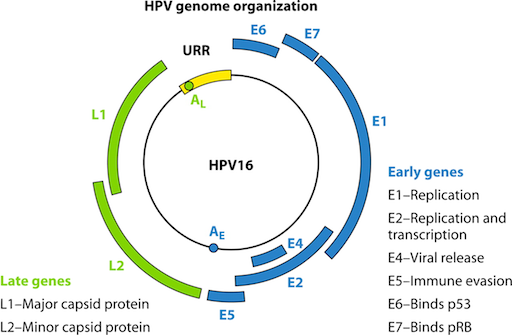
\includegraphics[scale=0.7]{IMG/genoma.png}
	\caption{Graphic illustrating the genomic organization of a typical mucosal high-risk HPV. The genome contains early (E) and late regions (L), which relate to the positions of the genes within the genome and their timing of expression during the viral life cycle. The early (E) region carries a number of genes which function at the level of viral replication and transcription, i.e., E2, E1, E6, and E7. E2 encodes a protein which has an auxiliary role in viral replication and also functions at the level of transcriptional regulation of the viral early genes. The E6 and E7 genes encode the major transforming proteins of the oncogenic HPVs. The late region (L) encodes viral structural proteins, with L1 being the major capsid protein and L2 being the minor capsid protein, adopted from 
	\cite{Stanley215}.}
	\label{genoma}
\end{figure}

The finding was followed by epidemiologists, molecular biologists, vaccinologists, and clinicians culminating in 2006 with the development of effective prophylactic vaccines for HPV, which have the means to prevent 70-80\% of cervical cancers \cite{olsen2015revisiting}. Zur Hausen was awarded the Nobel Prize in Physiology or Medicine in 2008, in recognition of his discovery.

\begin{figure}[ht]
	\centering
	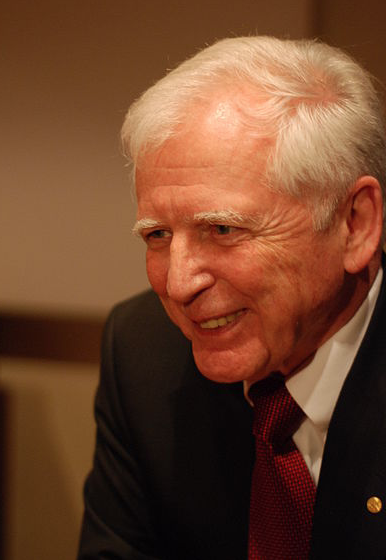
\includegraphics[scale=0.7]{IMG/zurHausen.png}
	\caption{Harald zur Hausen (born 11 March 1936) is a German virologist and professor emeritus. He has done research on cancer of the cervix, where he discovered the role of papilloma viruses, for which he received the Nobel Prize in Physiology or Medicine 2008. Adopted from \cite{haraldZur2010}}
	\label{zurHausen}
\end{figure} 
%Foto de Zur Hausen

% La ETS mas común del mundo
With more than 600 million cases worldwide, including 20 million in the United States, HPV is the most common STD, according to the Centers for Disease Control and Prevention (CDC) and the World Health Organization (WHO). More than 40 HPV types can infect the genital areas of men and women, including the skin of the penis, vulva, and anus, and the linings of the vagina, cervix, and rectum.

Most people who become infected with HPV do not know they have it. Usually, the body's immune system gets rid of the HPV infection naturally within two years. This is true of both high risk (HR) and low risk (LR) types. By age 50, at least 4 out of every 5 women will have been infected with HPV at one point in their lives. HPV is also very common in men, and often has no symptoms.

%Datos de lo malo que es
HPV types are often referred to as LR wart causing or HR cancer causing \cite{Clifford1157}, based on whether they put a person at risk for cancer. The types of HPV that can cause genital warts (GW) are not the same as the types that can cause cancer. Persistent HPV infections with genotypes 16 and 18 are responsible for about 70\% of all cervical cancer, with 40-85\% of other anogenital cancers: anal, penile, vaginal, and vulvar cancer, and also 16-28\% of the head and neck cancers \cite{olsen2015revisiting}. HPV is a cause of other non malignant diseases, to mention genotypes 6 and 11 cause about 90\% of anogenital warts \cite{lacey2006burden}.

\begin{figure}[ht]
	\centering
	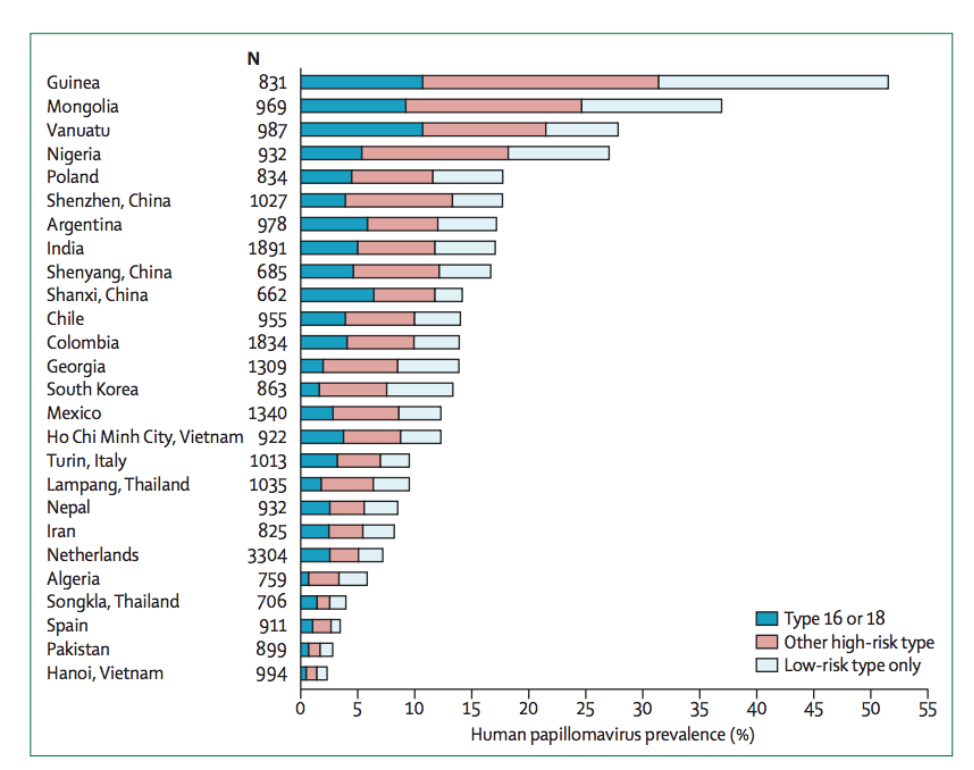
\includegraphics[scale=0.7]{IMG/prevalence.png}
	\caption{Age-adjusted prevalence of cervical human papillomavirus DNA in sexually active women aged 15-69 years. Data are from IARC Prevalence Surveys, 1990-2012, adopted from \cite{Marx1986HumanPV}.}
	\label{ageAdjusted}
\end{figure} 
%Foto de prevalencia

%Lo que cuesta $$$$
It is estimated that about 1 million new cases of GW are reported each year and the cost of treatment is increased by the tendency of these warts to recur after initial clearance. The cost of the treatment of GW was estimated to exceed \$ $3.8$ billion in the U.S. in $1997$ \cite{roberts1999vaccine}. In Spain there were $35,000$ cases in women in $2007$ with an overall annual cost of \euro \ $47$ millions \cite{castellsague2012prevalence}.

%Empiezo con las vacunas
\section{Vaccines and mathematical models}

Since the release of the first vaccines in 2006, nowadays there are three available: a quadrivalent (including HPV genotypes 16, 18, 6 and 11) and a bivalent vaccine (including genotypes 16 and 18) and a nonavalent (including genotypes 6, 11, 16, 18, 31, 33, 45, 52 and 58). All vaccines are efficacious to protect against precancerous lesions in the cervix, vulva or vagina; in addition, the quadrivalent and nonavalent prevent precancerous anal lesions, anal cancer and anogenital warts. 

%Two vaccines consisting of non-infectious HPV virus-like particles (VLP) \cite{mcneil2006invented} containing the capsid protein L1 of the virus but not the viral DNA. They induce a high immune response and prevent premalignant lesions. Both vaccines contain genotypes $16$ and $18$, and one of them adds VLP against genotypes $6$ and $11$ (HPV4).

According to the Advisory Committee on Immunization Practices (ACIP) from the Centers for Disease Control (CDC) and Prevention, new recommendations are given for use of a 2-dose schedule for girls and boys who initiate the vaccination series at ages 9 through 14 years. Three doses remain recommended for persons who initiate the vaccination series at ages 15 through 26 years and for immunocompromised persons.

The HPV vaccine induces a herd immunity effect in genital warts when a large number of the population is vaccinated. This aspect should be taken into account when devising new vaccine strategies, like vaccination at older ages or male vaccination. Numerous cost-effectiveness studies of HPV-vaccination have been published in other countries. However, few studies include the prophylactic effect of all HPV-associated diseases, or the impact of vaccinating men.

%Therefore, it is important to develop mathematical models with good predictive capacities. We devised a sexual contact network that was calibrated to simulate the Spanish epidemiology of different HPV genotypes. Through this model, we simulated the scenario that occurred in Australia in 2007, where 12-13 year-old girls were vaccinated with a three-dose schedule of a vaccine containing genotypes 6 and 11, which protect against genital warts, and also a catch-up program in women up to 26 years of age. Vaccine coverage were $73\%$ in girls with three doses and with coverage rates decreasing with age until $52\%$ for 20-26 year-olds. A fast $59\%$ reduction in the genital warts diagnoses occurred in the model in the first years after the start of the program, similar to what was described in the literature.%

In Spain HPV vaccine is given to adolescent girls as part of the national immunization programme, and is recommended at different age groups in different Autonomous Communities.
In the Region of Valencia, Spain, the vaccine is administered to $< 15$ girls. Similar vaccination strategies of this kind were modeled by Elbasha et al. \cite{elbasha2007model,elbasha2005vaccination} by means of a compartmental model with $17$ age groups for each gender. This model focuses mainly on the development of cervical intraepithelial neoplasia (CIN) and its progression from CIN1 to CIN3. According to these authors vaccination must be implemented for adolescent girls aged between $12$ and $14$ years. Elbasha et al. also found some evidences that the vaccination of boys could also be cost-effective \cite{elbasha2007model}. By vaccinating girls alone a $83\%$ reduction in the incidence of GW is expected but this reduction is increased to $97\%$ if boys are also vaccinated.

It is important to develop mathematical models with good predictive capacities. Some models have shown that the female vaccination program has some herd immunity and the impact of implementing the vaccination in males may not be cost effective. Besides, there is no economic analysis of the nonavalent program in Spain, and it is important from the decision making perspective.

Random network mathematical models may simulate the interactions and propagation of all these viruses through sexual contacts among a population of more than half million people (including heterosexual and homosexual populations). 

Before proceeding with the definition of our model, it is convenient to give a brief and general perspective on the emergent field of network research for the readers not familiar with these techniques and their application in epidemiology. A network is, basically, a model which derives from the abstract mathematical concept of a graph composed by a set of points (the so-called nodes) connected among them by some lines or edges (known as ``links'' in the case of networks).

\begin{figure}[ht]
	\centering
	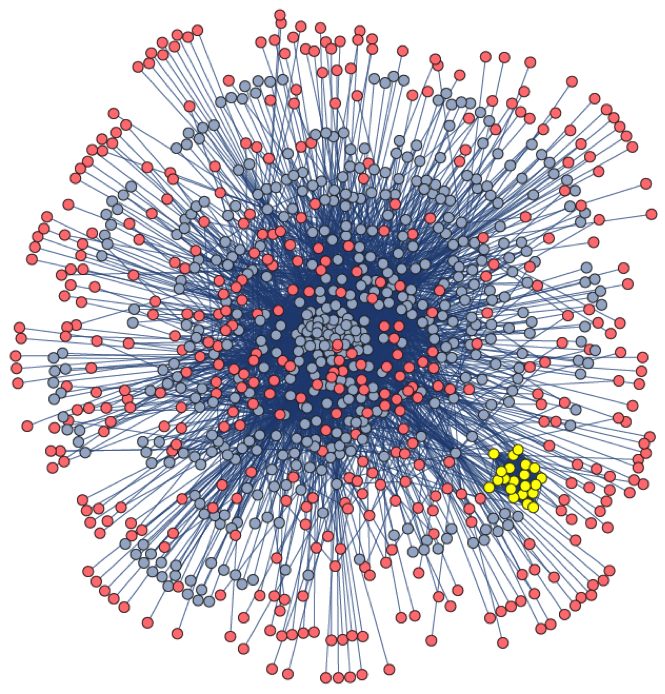
\includegraphics[scale=0.7]{IMG/LSPasd.png}
	\caption{Example Network of 1,000 nodes, MSM in yellow, women in red and men in blue.}
	\label{LSPnetwork}
\end{figure}


There are several types of networks of interest for the applied sciences. If we classify them according to the degree of a node, i.e., to the number of links for a given node (or, more properly, to the distribution of these number of links), we have two main categories in the literature: (i) random networks, in which the links or edges occur with a fixed probability and the statistical distribution of this number of links follows a Poisson's law; (ii) scale-free networks whose distribution of degrees follows a power-law with an algebraic tail of the form $P(k) \simeq 1/k^\gamma$ with $2 < \gamma < 3$. This means that the nodes with very large degrees are more likely to appear in scale-free networks than those in random networks. Random networks have been used in epidemiology \cite{acedo2011using} and also as an elementary model of the brain \cite{acedo2013brain}. On the other hand, scale-free networks have been successfully applied to the Internet and biological networks in which some nodes with a very large number of links are determinant in the control of the dynamics (see \cite{dorogovtsev2013evolution}) and (iii) small-world networks referring to the average length of a path connecting two typical nodes in the network. Small-world networks are an important paradigm in the science of networks. It was found that some sparse networks may present the small-world phenomenon, i.e., there are short paths connecting every pair of nodes through the links with other nodes. A mechanism to generate these networks was discovered by Watts and Strogatz \cite{watts1998collective}. Many networks in sociology exhibit this small-world property \cite{christakis2007spread,liljeros2001web,bearman2004chains}.

STD are more likely to produce large-scale infections than other transmissible diseases, such as respiratory transmitted diseases, because the efficacy of sexual contacts for the infection is large and the infectious agent has long latency periods as in the case of HIV or HPV. Moreover, neither the carrier nor his/her partner are aware of their exposure. For example, it has been estimated that around $40-50\%$ of contacts are capable of transmitting HPV \cite{burchell2006modeling}.

In order to predict the evolution of these diseases we need a reliable model of the underlying social network in which the infection builds up. Individuals who change partners or have several partners simultaneously, are the hubs favoring the spread of STD. The distribution of degrees of the nodes in the network and the average chemical path from an infected individual to a susceptible one, are important parameters controlling the final extension of a new STD in a population and the speed at which it spreads. However, most models are based on some assumptions, which could not be valid for certain populations. Some studies claimed that the web of human sexual contacts is a scale-free network characterized by a power-law distribution for the number of individuals with a certain degree of connectivity, $k$: $P(k)\propto 1/k^\alpha$ with a value of $\alpha$ in the range $2 <\alpha < 3$, and slightly smaller for males than for females \cite{liljeros2001web}. Although $P(k)$ provides some valuable information about the network, it is not a sufficient prescription on how to build it for a given population size. Moreover, a power-law distribution of contacts could not be representative of some populations, or could vary from country to country. For example, it has been found that a densely connected core appears without the need of a high connectivity degree in the Jefferson High School's network \cite{bearman2004chains}. 

Even with the high prevalence of STDs there are few studies devoted to ascertain the structure of sexual networks and its role in disease transmission. Most studies are restricted to small communities such as the Jefferson High Schools project \cite{bearman2004chains} or that of Likoma Island \cite{helleringer2007sexual}.

Some field studies have ascertained the structure of moderate size real networks of sexual contacts. In $2004$, Bearman et al. published the results for a set of $800$ adolescents in a mid sized town of the United States \cite{bearman2004chains}. They  showed that the structure of this network is a big cluster with a ring and extended filaments which contained most of the adolescents implying that, potentially, the infection of an individual could spread to the whole of the population, given sufficient time and infectivity. A similar study was performed in $2007$ at the Likoma Island in Malawi with the idea of predicting and explaining the expansion of HIV in sub-Saharan populations \cite{helleringer2007sexual}. That study disclosed  that the sexual network contained many cycles, in contrast with the single cycle at Jefferson High School. For that reason, it was speculated that superimposed cycles could be the explanation of the high prevalence of HIV infection in small populations of Africa.

Some recent studies reveal that the evolution of partnerships is also an important factor in the transmission of STDs. In particular, they pointed out that the following items should be considered: (i) the cumulative distribution of the lifetime number of partners, (ii) the distribution of partnership duration, (iii) the distribution of gap lengths between partnerships, and (iv) the number of recent partners. A method for building up networks considering these items has been developed by Schmid and Kretzschmar \cite{schmid2012determinants}. However, this information is not available in most surveys, and we therefore face the problem of developing reasonable models for STDs in many countries where information about sexual behaviour is scarce. For example, in the case of Spain, there is only available data about the number of sexual contacts in a lifetime from surveys. This is sufficient for building a sexual network for the transmission of HPV or other diseases with lifetime consequences and progression. In these cases, the important fact is whether the individual has had a contact with risk of infection. The remaining aspects of the network such as the duration of partnership and the time intervals among them can be incorporated effectively into a probability of transmission parameter.

%Network models are those models in which the relations of the individuals (represented by network sites) are taken into account by means of the network bonds. Random network models have been successfully applied to other infectious diseases such as the Respiratory Syncytial Virus pandemic \cite{acedo2011using} as well as other social pandemics such as obesity \cite{christakis2007spread}.

%Recuerda que el esfuerzo de construir el modelo de redes es porque se está observando que hay resultados del efecto de la vacuna mucho antes de lo que decía el modelo existente (Elbasha et al.), la aparición del debate de la vacunación de niños, que el modelo de Elbasha et al. no aporta mucho y que dicho modelo no explica bien el efecto comunitario. Esas cosas no las he visto claramente en la introducción.
\section{Our proposal}

In recent studies \cite{ali2013genital,fairley2009rapid} a decrease on the number of infected persons and the number of persons with GW is already reported for Australia after two years of administering vaccinations to young girls. It showed both direct and indirect protection in males. These results were more impressive than the predictions of the continuous models. New vaccination schedules, specially vaccination in boys, should take into account the herd immunity effect vaccination in girls (in mainly heterosexual societies). 

A Bayesian model for HPV vaccination was then proposed by Bogaards et al. \cite{bogaards2015direct} and focused on the herd immunity effect of the female vaccination on the male population in a static picture. A dynamic understanding for the short and long term effects of vaccination policies is, however, still necessary and even more so with HPV vaccines because their benefit to the whole population is to be observed in the time span of several decades.

In this dissertation we propose a model based upon a network instead of traditional continuous models. We show how to build a network model for sexual contacts from the usual statistical data in surveys concerning the number of partners in a lifetime. We consider both heterosexual men and men who have sex with men (MSM) populations and the connections among them. We perform simulations over this network substrate on the HPV infections by different genogroups including both LR and HR infections. We will be able to determine with higher accuracy the effect of vaccination in a short and large periods of time, this is, the herd immunity effect. In particular, we show that for the case of Australia the strategy of a vaccination for $12-13$ year-old girls plus catch-up lead to a considerable reduction in the number of cases of infection by HPV 6 and/or 11 (which are the main cause of GW). For women in the $14-26$ age-group we obtain a decrease of $59\%$ after $3.6-4.6$ years and $39\%$ in men after $3-3.75$ years. These results agree with the conclusions of the study by Ali et al. \cite{ali2013genital}.

In the following chapters we will explain in detail: 
\begin{itemize}
	\item the building of the network model for sexual contacts. This is a technical-computational chapter;
	\item how the calibration of the model is carried out. This is a technical-computational chapter;
	\item model validation simulating the Australian scenario and obtaining similar results;
	\item the study of the decline of warts with the current vaccination campaign in Spain: vaccination of girls with a coverage of $70\%$;
	\item the study of the decline of oncogenic HPV with the current vaccination campaign in Spain;
	\item the study of what would happen if the effect of the vaccine disappear suddenly after $20$ years;
	\item the study about if the tourism in Spain has a significant effect on the HPV infection;
	\item the study of the decline of oncogenic HPV if we vaccinate boys and girls with a high coverage;
	\item the study of how long the decline is recovered after a drop in the coverage;
	\item the study of how change the decline of HPV if the average number of LSPs increases significantly;
	\item the study of how change the decline of HPV if the number of MSMs increases significantly.
\end{itemize}



%Cap�tulo 2
% !TeX spellcheck = en_US
\chapter{Building LSP networks and describing the transmission dynamics of HPV on these networks}\label{ConstruccionYDinamica}

\section{Origin of the data}

%me enrollo un poco mas
Building a social network requires demographic data, for this model we have used data from the region of Valencia (Spain) that was collected from the Valencian Institute of Statistics (2013) \cite{IVE}, from this set of data we are interested in the distribution of males and females along with their age. The second set of data for this model has to do with sexual habits, this is the LSP for an individual, which was obtained from the Health and Sexual Habits Survey of 2003 \cite{INE}, and summarized in Tables \ref{tableLSPValues_men} and \ref{tableLSPValues_women}. 

\begin{table}[H]
	\centering
	\begin{tabular}{ccccccc}
		\multicolumn{7}{c}{MEN} \\
		\midrule 
		Age & $0$ LSP & $1$ LSP & $2$ LSP & $3-4$ LSP & $5-9$ LSP & $10+$ LSP \\
		\midrule
		14--29 & 0.107 & 0.207 & 0.131 & 0.225 & 0.168 & 0.162 \\
		30--39 & 0.027 & 0.225 & 0.128 & 0.21 & 0.17 & 0.24 \\
		40--65 & 0.019 & 0.268 & 0.14 & 0.193 & 0.163 & 0.217 \\
	\end{tabular} 
	\caption{Proportion of men per number of lifetime sexual partners (LSP) per age group. Note that the sum of the rows are 1.}
	\label{tableLSPValues_men} 
\end{table}

\begin{table}[H]
	\centering
	\begin{tabular}{ccccccc}
		\multicolumn{7}{c}{WOMEN} \\
		\midrule 
		Age & $0$ LSP & $1$ LSP & $2$ LSP & $3-4$ LSP & $5-9$ LSP & $10+$ LSP \\
		\midrule
		14--29 & 0.138 & 0.43 & 0.186 & 0.158 & 0.056 & 0.032 \\
		30--39 & 0.029 & 0.501 & 0.168 & 0.177 & 0.077 & 0.048 \\
		40--65 & 0.017 & 0.652 & 0.138 & 0.118 & 0.039 & 0.036 \\
	\end{tabular} 
	\caption{Proportion of women per number of lifetime sexual partners (LSP) per age group. Note that the sum of the rows are 1.}
	\label{tableLSPValues_women} 
\end{table}

Some features of the distribution of contacts were: (i) the percentage of males and females with no partners is
very similar in each age-group; (ii) the proportion of women  with a single partner is, approximately, two times larger than men with only one partner; and (iii) the percentage of men with two or more partners is always larger than that of women except for women in the age-groups 14--29, and~30--39 in the case of two partners. The asymmetry in the behaviour of males and females should be taken into account in the construction of the network.

\section{Network model}

In this dissertation, we use the random network model as a basis to simulate the network of sexual contacts among individuals, but, in this model, the average number of connections depend upon the age-group as deduced from Tables \ref{tableLSPValues_men} and \ref{tableLSPValues_women}. A basic property of the network we are going to discuss is that the total number of LSP for the male population (M) must coincide with the total number of LSP for the female population (F). This is so because (in a purely heterosexual network) every link starting on a male must end in a female and vice versa. In mathematical terms:

\begin{equation}
\label{nodeseq}
\displaystyle\sum_{i=1}^M\, LSP_i=\displaystyle\sum_{j=1}^F\, LSP_j\; .
\end{equation}

About the estimation of sexual partners, there are some approaches to the number of LSP in males and females \cite{chandra2013sexual,mosher2005sexual} that are difficult to match. Generally speaking, males tend to overestimate the number of their sexual partners and females tend to underestimate it. Therefore, we considered the average LSP male value, $\left\langle k \right\rangle_m$, and calibrated the network so that results were consistent with data of Tables \ref{tableLSPValues_men} and \ref{tableLSPValues_women}, and estimated that the number of LSP in males in Spain was at least $4.5$. Networks with 100,000, 250,000, 500,000 and 750,000 have been used during the present study. It required a substantial computational power.

\section{Semi-Random Construction}
\label{subsec22}

From Table \ref{tableLSPValues_men} (proportion of male LSP aged 14--29), we have the following list:
$( 0.107, 0.314, 0.445, 0.67, 0.838, 1)$ for the accumulated proportion of males less than or equal to a given LSP number.
Now, we randomly generate a number $r$ between $0$ and $1$ and assign the number of contacts to every male node in the $14-29$
age group, in the network as follows:

\begin{itemize}[leftmargin=*,labelsep=5mm]
\item $r \le 0.107$ say that the corresponding male does not have an LSP,
\item $0.107 < r \le 0.314$ say that the corresponding male has one LSP,
\item $0.314 < r \le 0.445$ say that the corresponding male has two LSPs,
\item $0.445 < r \le 0.67$  say that the corresponding male has three or four LSPs uniformly distributed.
\item $0.67 < r \le < 0.838$ say that the corresponding male has five to nine LSPs uniformly distributed.
\item $0.838 < r \le 1$ say that the corresponding male has 10 or more LSPs.
\end{itemize}

Every node in the network is labeled by its gender and age randomly assigned according to the population histogram. The assignment of the number of bonds, as another label of the node, is not so straightforward since we must guarantee that the condition in Equation\ (\ref{nodeseq}) is verified. In~order to fulfill this condition, we take advantage of the uncertainty of statistics reports concerning individuals with $10$ or more LSPs.

Starting with the males, we assign the number of LSPs up to nine partners and, for $10$ or more partners proceed as follows: let $i_{\mbox{max}}$ be the number of males with nine or less partners. The unassigned males should be $M-i_{\mbox{max}}$ and the number of bonds that should be distributed among them is $M \left\langle k \right\rangle_m-\sum_{i=1}^{i_{\mbox{max}}}\, LSP_i$. By Euclidean division, this quantity can be expressed as $(M-i_{\mbox{max}}) n_m+r_m$, where $n_m \ge 10$. In our procedure, we assign a random number of bonds, uniformly distributed, in the interval $\left[10,2 n_m-10\right]$ to every male with $10$ or more LSPs, i.e.,
to~the $M-i_{\mbox{max}}$ unassigned males.

Now, we denote as $p_m$ the total number of bonds of the male population. We must take into account, as expressed in Equation\
(\ref{nodeseq}), that the total number of bonds of the female population should be the same. To impose that condition, we
proceed as follows: (i) assign the number of bonds to the females with nine or less partners following the statistical 
data in Tables \ref{tableLSPValues_men} and \ref{tableLSPValues_women}; (ii) the sum of all female LSPs in this group of $j_{\mbox{max}}$ members will be denoted by $s_f$. 
Then, $n_f=F-j_{\mbox{max}}$ is the number of females with $10$ or more LSPs; (iii) the number of bonds starting in the males and still unassigned to a female is $p_m-s_f= q_f n_f + r_f$, where $0 \le r_f < n_f$ and $n_f \ge 10$; (iv) we assign $q_f+1$ bonds to $r_f$ females still unassigned and $q_f$ bonds to the rest of $n_f-r_f$ females. The steps of this algorithm are also enumerated in the flow diagram in Figure  \ref{flux1}.

Notice that, for men and women with more than 10 LSPs, we assign their LSP in the most equitable way, assuming that all of them have, more or less, the same number of LSPs. Thus, we have a lot of hubs with a low number of contacts instead of a few hubs with a lot of contacts.

From the point of view of STD transmission, the latter situation leads to a faster transmission if the hub is infected, and, also, if the hub is vaccinated, the transmission is cut faster. Therefore, due to the lack of data about people with $10$ or more LSPs, we make the decision of being conservative in the transmission of the disease and in the effect of the vaccination campaigns.

Notice that this procedure implies that the condition in Equation\ (\ref{nodeseq}) is verified. After this procedure, we have obtained the following lists:
\begin{itemize}[leftmargin=*,labelsep=5mm]
\item $AgeMale\left[ i \right]$ is the age of the i-th male, $i=1,\ldots,M$,
\item $AgeFemale\left[ i\right]$ is the age of the i-th female, $i=1,\ldots,F$,
\item $kMale\left[ i \right]$ is the number of LSP for the i-th male, $i=1,\ldots,M$,
\item $kFemale\left[ i \right]$ is the number of LSP for the i-th female, $i=1,\ldots,F$.
\end{itemize}

These lists will be used to perform the connections of males and females and build the network. Note that, in Tables \ref{tableLSPValues_men} and \ref{tableLSPValues_women}, there are more females than males with few LSPs (comparing male and female percentages). It implies that there will be few women with a very large number of LSPs. This fact suggests us to start the assignment procedure with women with the largest LSPs. Otherwise, it would be possible that, when we have to assign LSPs of men to a female with a large number of LSPs, there~will not be enough men with free sexual partners to be assigned and, for this female, it would be impossible to satisfy the condition that the degree of each node was the number of its LSP. 

\begin{figure}[H]
	\centering
	\begin{tabular}{c}
		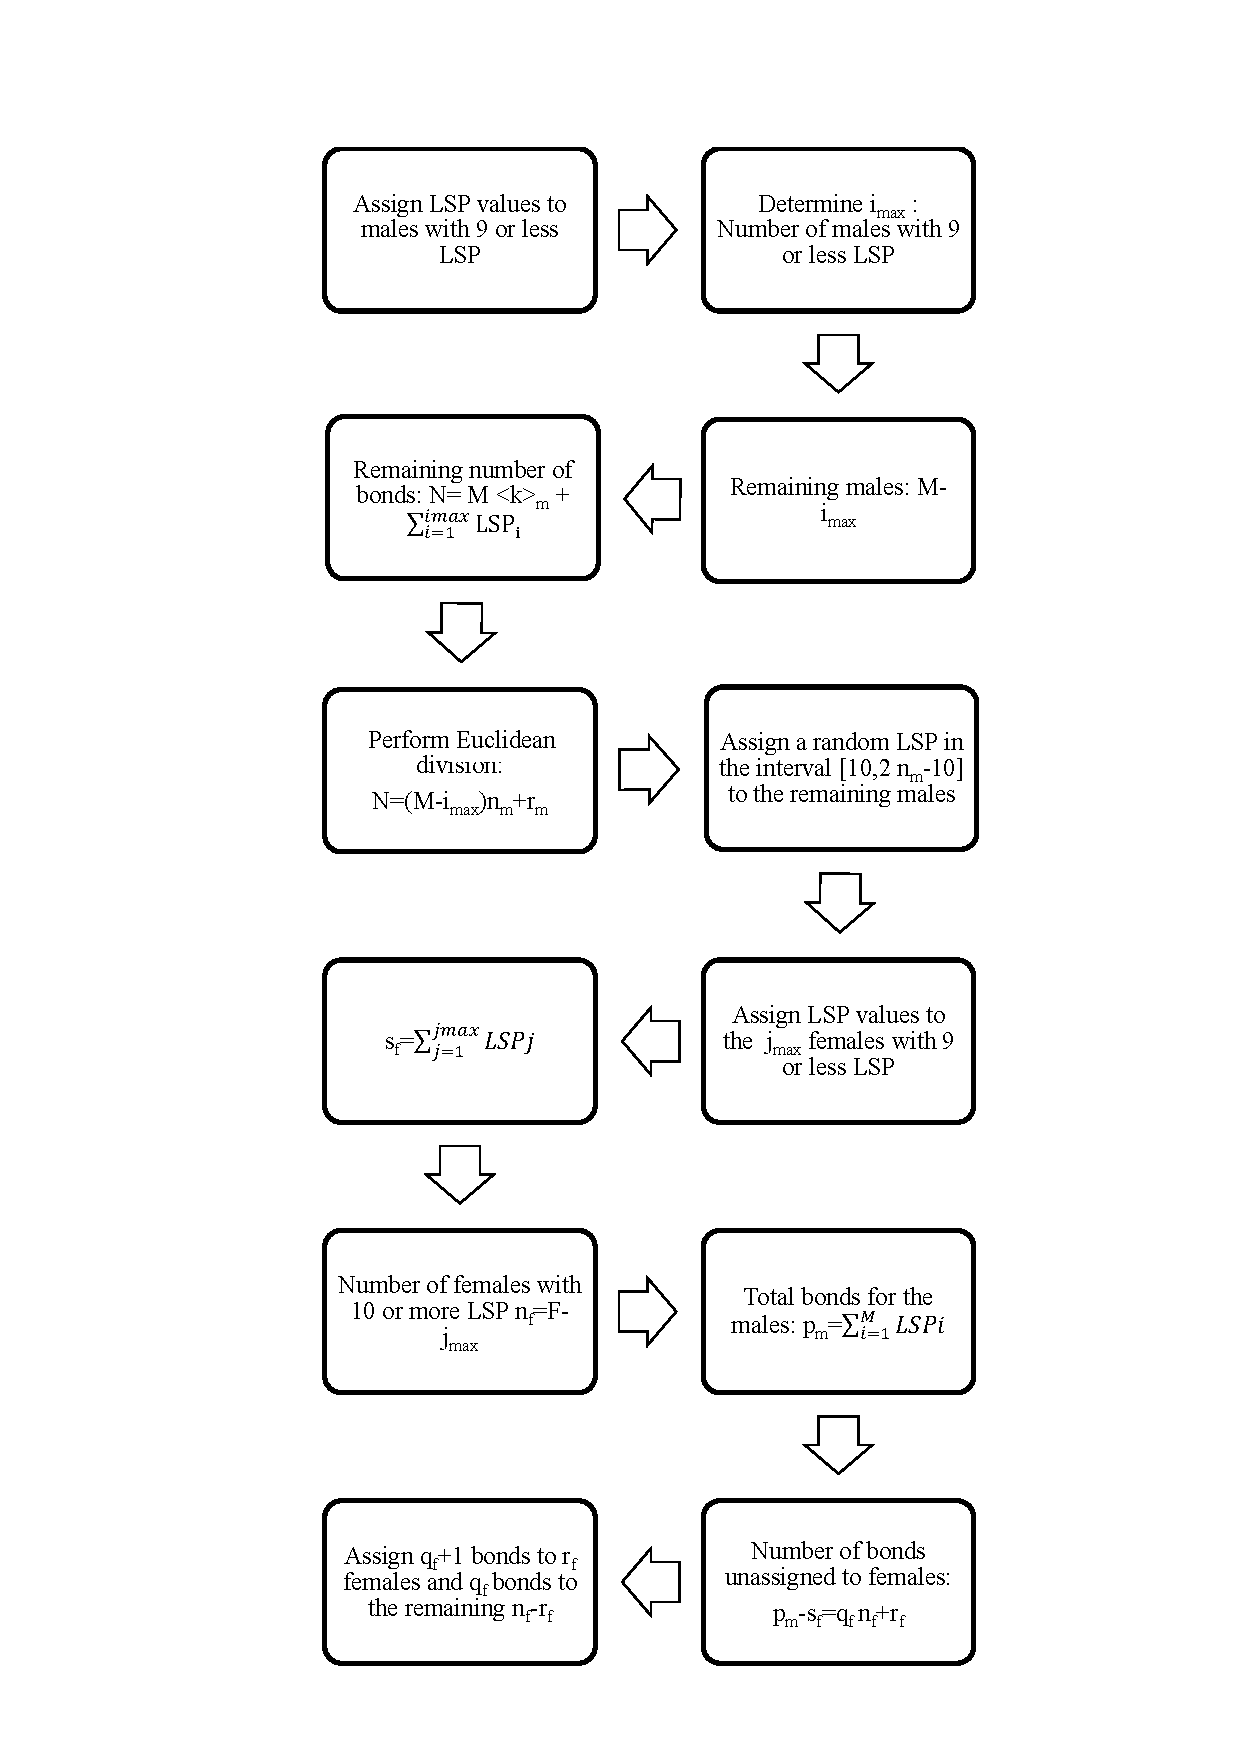
\includegraphics[width=\textwidth]{IMG/FluxDiagramI.pdf}
	\end{tabular}
	\caption{Flow diagram for the algorithm corresponding to the assignment of a number of LSPs to every male and female in the network.\label{flux1}}
\end{figure}

The assignment of partners was carried out by considering a principle of psychological similarity~\cite{gentner1997structure} or assortativity.
Hence, we are going to define a weight function assuming that: women with few LSPs usually match men with few LSPs; people with four or more LSPs use to join with people with four or more LSPs; and couples where one of them has a large number of LSPs and the other few LSPs will be uncommon. Then, for the woman $i$ and the man $j$, we define the following weight~function:

\begin{equation}
\pi(i,j) = 
\begin{array}{l}
\left\lbrace \begin{array}{lc}
| kFemale[i] - kMale[j] | & kFemale[i], kMale[j] \le 4 \\
0 & kFemale[i], kMale[j] > 4 \\
100 & \mbox{otherwise}
\end{array} \right\rbrace, \\
\\
 + | AgeFemale[i] - AgeMale[j] - 1.8 |.
\end{array}
\label{peso}
\end{equation}

The combined weight function, which takes into account the age difference of the partners, $\vert AgeFemale[i] - AgeMale[j] - 1.8 \vert$ is defined in this way because some studies show that the average age difference among the members of a couple in Spain is $1.8$ years \cite{miret2010similitud}. 

%The MSM population (around $3.88$ \% of the total male population in Spain)\cite{INE} can also be incorporated into the model, but, in this subpopulation, the connectivity would be larger than the heterosexual network. The MSM population would also be connected with the heterosexual one by links with women in such a way that every MSM individual has a link with a woman with five or more contacts \cite{acedo2017calibrating}.

The estimated percentage of men who have sex with men (MSM) is $3.88\%$  \cite{INE}. The situation for the MSM population is different of the one shown in Tables \ref{tableLSPValues_men} and \ref{tableLSPValues_women}, because the average number of sexual partners is estimated in 39 regardless of age, but this number increases with age with a peak of 59 in the 40-49 age-group \cite{Durex2002}.
A difficulty arises because we have little information about the number of sexual contacts of women who have sex with women (WSW) subpopulation. In a personal communication by Dr. Mireia D\'iaz from the Catalan Institute of Oncology (IDIBELL) we were informed that HPV hardly spreads among WSW, and almost all MSM, sometimes in their lives, had a woman partner. Consequently, we have simulated these connections by assigning a contact to every man in the MSM subpopulation with woman with 5 partners or more. This is done according to the assortativity principle, that is, people use to join with people with similar habits.

The assignment of links is then performed by the Greedy Randomized Adaptive Search Procedure (GRASP) algorithm \cite{cormen2009introduction,feo1995greedy}. %Details about the construction of the whole network have been provided in previous studies \cite{acedo2017calibrating,BuildingLSPNova}. 


%Cap�tulo 3 
% !TeX spellcheck = en_US
\chapter{Calibrating the Sexual Contacts Network }\label{Calibrado}

The calibration of this kind of random computational models is an open problem and several issues about fitting computational models to data with uncertainty have to be addressed. For instance, 

\begin{itemize}
	\item the fact that, for the same set of parameters, different realizations usually return different outputs, and consequently, one realization may fulfill the fitting requirements and another realization does not,
	\item the determination of an appropriate measure of goodness-of-fit,
	\item to find model parameters agreeing the values appearing in the medical literature in a reliable and reproducible way,
	\item adaptation of the optimization algorithms to these above issues and the available resources,
	\item the determination of the best parallel implementation of the optimization algorithms, in terms of quality of the solutions and computational efficiency of the program.
\end{itemize} 

In the remainder of this section, we are going to describe thoroughly the procedure we propose to approach the above issues.

\section{Description of the model}\label{sec:modelo}
As we explained in Chapter \ref{ConstruccionYDinamica}, we described how to build lifetime sexual partners (LSP) networks. These networks are built with the main aim to reproduce the demography in Spain \cite{IVE}, and data about the LSP, for men and women, and for age groups $18-29$, $30-39$ and $40-65$, presented in a survey about sexual habits in Spain \cite{INE} and collected in Tables \ref{tableLSPValues_men} and \ref{tableLSPValues_women}. 

Then, over the LSP network, we describe the dynamics of the HPV \cite{Acedo2017,DezDomingo2017}. We divide the nodes into the age groups $14-17$, $18-29$, $30-39$, $40-65$. For the implementation of the simulation of the transmission of HPV among the individuals in the network, a standard epidemiological model with susceptible and infected states and three types of infections (HR, LR and co-infection) was carried out. The epidemiological model is defined by a set of parameters, hence, it is necessary to include $11$ model parameters that will address the transmission dynamics of HPV on the LSP networks:

\begin{enumerate}
	\item Average number of men LSP, needed for network LSP building.
	\item We need some probabilities to determine if a sexual partner is going to produce a contagion to another partner in a given time stage. These parameters are different for each age group:	
	14--17, 18--29, 30--39 and 40--65. Notice that this means that the probability of contagion depends upon the age group of the members of the relationship. Moreover, the probability of connection of these members in the network is also age-dependent as proposed in Equation (\ref{peso}). The values of these probabilities are determined in the process of the model calibration.\label{las_T}
	\item Average time an individual infected by a high (low) risk HPV clears the infection and recovers (2 parameters).
	\item Probability that a woman (man) infected of high (low) risk HPV transmits it to his/her partner in a sexual intercourse (4 parameters). 
\end{enumerate}

Most of the above parameters have been studied in the literature and there are some estimations we have to take into account:
\begin{itemize}
	\item The average number of men LSP: it is around $8$ \cite{Durex2002}. For this parameter, our search will be in the interval $[7, 10]$.

	\item The time for clearing the infections due to HPV HR, for both men and women: in \cite{elbasha2007model}, the authors say that the mean duration of HPV 16/18 infection is $1.2$ years; in \cite{Giuliano2011}, the mean duration of HPV 16 is $12.19$  months $(7.16-18.17)$; in \cite{Nyitray2015} the duration clearance varies, in average, between $6.5$ months to $11.8$ months. Thus, we considered the interval $[0.8, 1.2]$ years.
	
	\item The time for clearing the infections due to HPV LR, for both men and women: in \cite{elbasha2007model}, the mean duration of HPV 6/11 infection is $0.7$ years; in \cite{Giuliano2011}, the mean duration of HPV infection is $7.52$ months $(6.80-8.61)$ for any HPV;  in \cite{Nyitray2015} the duration clearance varies, in average, between $6.2$ months to $11.7$ months. Thus, we considered the interval $[0.5, 1]$ years.
	
	\item In \cite{elbasha2007model}, the authors estimated the probability of HPV infection transmission per partnership and by type and, as in \cite{castellsague2012prevalence}, this probability is higher for transmission from males to females $(0.8)$ than that for transmission from females to males $(0.7)$. Given that these data come from estimations (not surveys) and after some runs of our model, we are going to be more flexible and consider the probability interval $[0.2,0.6]$ for LR transmission and $[0.5,1.0]$ for HR transmission, given that, women transmit less than men.
\end{itemize}

Simulations are executed by generating a network and carrying out a large number of epidemic evolution time-steps starting with a number of individuals infected by both HPV types as given by the CLEOPATRE study \cite{castellsague2012prevalence}.
After the warm-up period, we obtain a stable situation and we can proceed with the calibration by comparing the model predictions with real data and deducing the most probable values of the set of parameters.

We have used a calibration procedure using the Particle Swarm Optimization (PSO) algorithm \cite{khemka2008exploratory}. The prevalence data for each age group is listed in Table \ref{datosConstruccion}.

\begin{table}[H]
	\centering
	\begin{tabular}{cccc}
		\toprule
		\textbf{Women} & \textbf{HR-Infected} & \textbf{LR-Infected} \\
		\midrule
		18--29 y.o. & $24.10\%,$ $[21.33\%, 26.98\%]$ & $6.36\%,$ $[4.71\%, 8.07\%]$ \\
		30--39 y.o. & $11.01\%,$ $[7.54\%, 15.09\%]$ & $1.26\%,$ $[0.0\%, 3.14\%]$ \\
		40--64 y.o. & $5.96\%,$ $[4.29\%, 7.8\%]$ & $2.37\%,$ $[1.22\%, 3.68\%]$ \\
		\midrule
		18--64 y.o. & $16.23\%,$$[14.52\%, 17.97\%]$ & $4.41\%,$ $[3.42\%, 5.45\%]$ \\
		\bottomrule
	\end{tabular}
	\caption{Prevalence of HR- and LR-infected women per age groups from the 
		CLEOPATRE study \protect\cite{castellsague2012prevalence}. Co-infections are included in both HR- and LR-infected, mean and $95\%$ confidence intervals.}
	\label{datosConstruccion}
\end{table}

Note that the network building and the transmission parameters involve randomness and uncertainty due to the random processes used in the network building and the transmission dynamics of the HPV. This fact is going to be taken into account in the  calibration and simulation.

\section{Description of our resources}

\subsection{Computers}
All the realizations are going to be executed on two computers with 64 cores on 8 Xeon Sandy Bridge E5-4620 running at 2,2 Ghz, with 16 MB of cache memory and 512 GB RAM memory\footnote{Both computers are not exactly the same. There are some minor hardware differences.}. The operating system is Ubuntu Server 16.04 LTS. 

\subsection{Distributed computing environment}
We also have deployed a distributed computing environment called Sisifo. Sisifo is a client-server based system designed to allow a problem to be solved using distributed computation. Sisifo is able to assign tasks to a set of personal computers (PCs), wait for the tasks to be completed and collect the results for further analysis. Sisifo is made with simplicity as main aim, giving as a result a system that requires almost no maintenance, needs very little configuration time, and can be deployed in just a couple of hours.

The Sisifo Server keeps listening for request of the clients. The Server has stored one or more executors, a set of problems to be solved in the \textit{Problem files} folder, and the solutions sent in the \textit{Result files} folder. 

The Sisifo Client is a program stored in one or several PCs that connects to the server, and asks for a \textit{work packet}. This work packet is composed of two elements: a text file containing the model parameter values and the simulator executable file. The Client, once the work packet is received, executes a realization using the model parameters stored in the text file. When the realization finishes, a solution file is generated, returned to the server and dropped in the \textit{Results files} folder. More details about how Sisifo works can be found in \cite{villanueva2013epidemic}.

In our case, the Sisifo clients are going to be located in each one of the 64 cores of the Sandy Bridge computers. The Sisifo server is located in a regular PC with MS-Windows 7.

\subsection{Random Particle Swarm Optimization (rPSO)}
Using Python3 \cite{python3} and \textit{Mathematica} \cite{Mathematica}, we have implemented an asynchronous version of rPSO adapted to the  \textit{Sisifo} computing environment. To do that, first, we recall the random PSO (rPSO) algorithm appearing in \cite{khemka2008exploratory} applied to the optimization of a function $F$.

\begin{description}
	\item[Step 1.] Initialization.
	\begin{itemize}
		\item Initialize $N$ particles $p_1, \ldots, p_N$ chosen randomly in the parameter space.
		\item Initialize randomly their velocities $v_1, \ldots, v_N$.
		\item Evaluate the fitness of all the particles $F(p_1), \ldots, F(p_N)$.
		\item Define the individual best fitness as $p_i^{best} = p_i$, $i=1,\ldots,N$ and the global best fitness $p_{global}^{best}$ as the $p_i^{best}$ which fitness is optimum.
	\end{itemize}
	\item[Step 2.] Modify the particle velocities based on the previous individual best and global best positions: 
	\[v_i = \omega v_i + \psi_1 ( p_i^{best} - p_i ) + \psi_2 ( p_{global}^{best} - p_i ), \ i=1,\ldots N, \]
	where $\omega$ is a random value in $[\frac{1}{4}, \frac{3}{4}],$ $\psi_1$ is the exploitation rate and $\psi_2$ is the exploration rate, both randomly generated in each iteration as a number in the interval $[0,1.5]$.
	\item[Step 3.] Update the particle locations: $p_i = p_i + v_i,$  $i=1,\ldots N$. 
	\item[Step 4.] Evaluate the fitness of all the particles $F(p_1), \ldots, F(p_N)$. 
	\item[Step 5.] Update the individual best fitness $p_i^{best}$, $i=1,\ldots,N$ and  the global best fitness $p_{global}^{best}$. Go to Step 2. 
\end{description}

The above algorithm can be adapted to \textit{Sisifo} computing environment if, using the \textit{Sisifo Server}, the computation of the fitness of the particles is distributed among the \textit{Sisifo Clients}.

However, in a typical PSO procedure, including rPSO, the set of particles is updated once the fitnesses of all the particles have been calculated. This means that, until all the fitnesses have not been evaluated and Step 4 is not completely finished, the particles cannot be updated and new evaluations cannot be performed. Then, in every iteration of rPSO, scenarios where some \textit{Sisifo} clients have finished their evaluations and are idle while other \textit{Sisifo} clients are still performing their evaluations will be common. In these scenarios, we have an under-use of the \textit{Sisifo} system.

In order to avoid the under-use system drawback, we propose the implementation of an asynchronous version of rPSO in such a way that when the fitness of a particle has been evaluated (Step 4), this particle is updated (Steps 5, 2 and 3) without waiting for the evaluation of the remainder particles, considering the current existing global best and its individual best particles. This way, we modify rPSO algorithm parallelizing Steps 2, 3, 4, 5 and sharing the updates of the global best particle.

We show in Figure \ref{rPSO.python} how we set the asynchronous rPSO in the \textit{Sisifo} environment. As we can see, the rPSO procedure generate the problems and write them into the \textit{Problem files} folder to be processed by the \textit{Sisifo Server}. Once the evaluation has been carried out and the solution file is in the \textit{Result  files} folder, rPSO reads the content of the solution file, analyses it and calculates the fitness. With this information, rPSO is able (Steps 2 and 3) to generate a new problem file. 

\begin{figure}[h!]
	\centering
	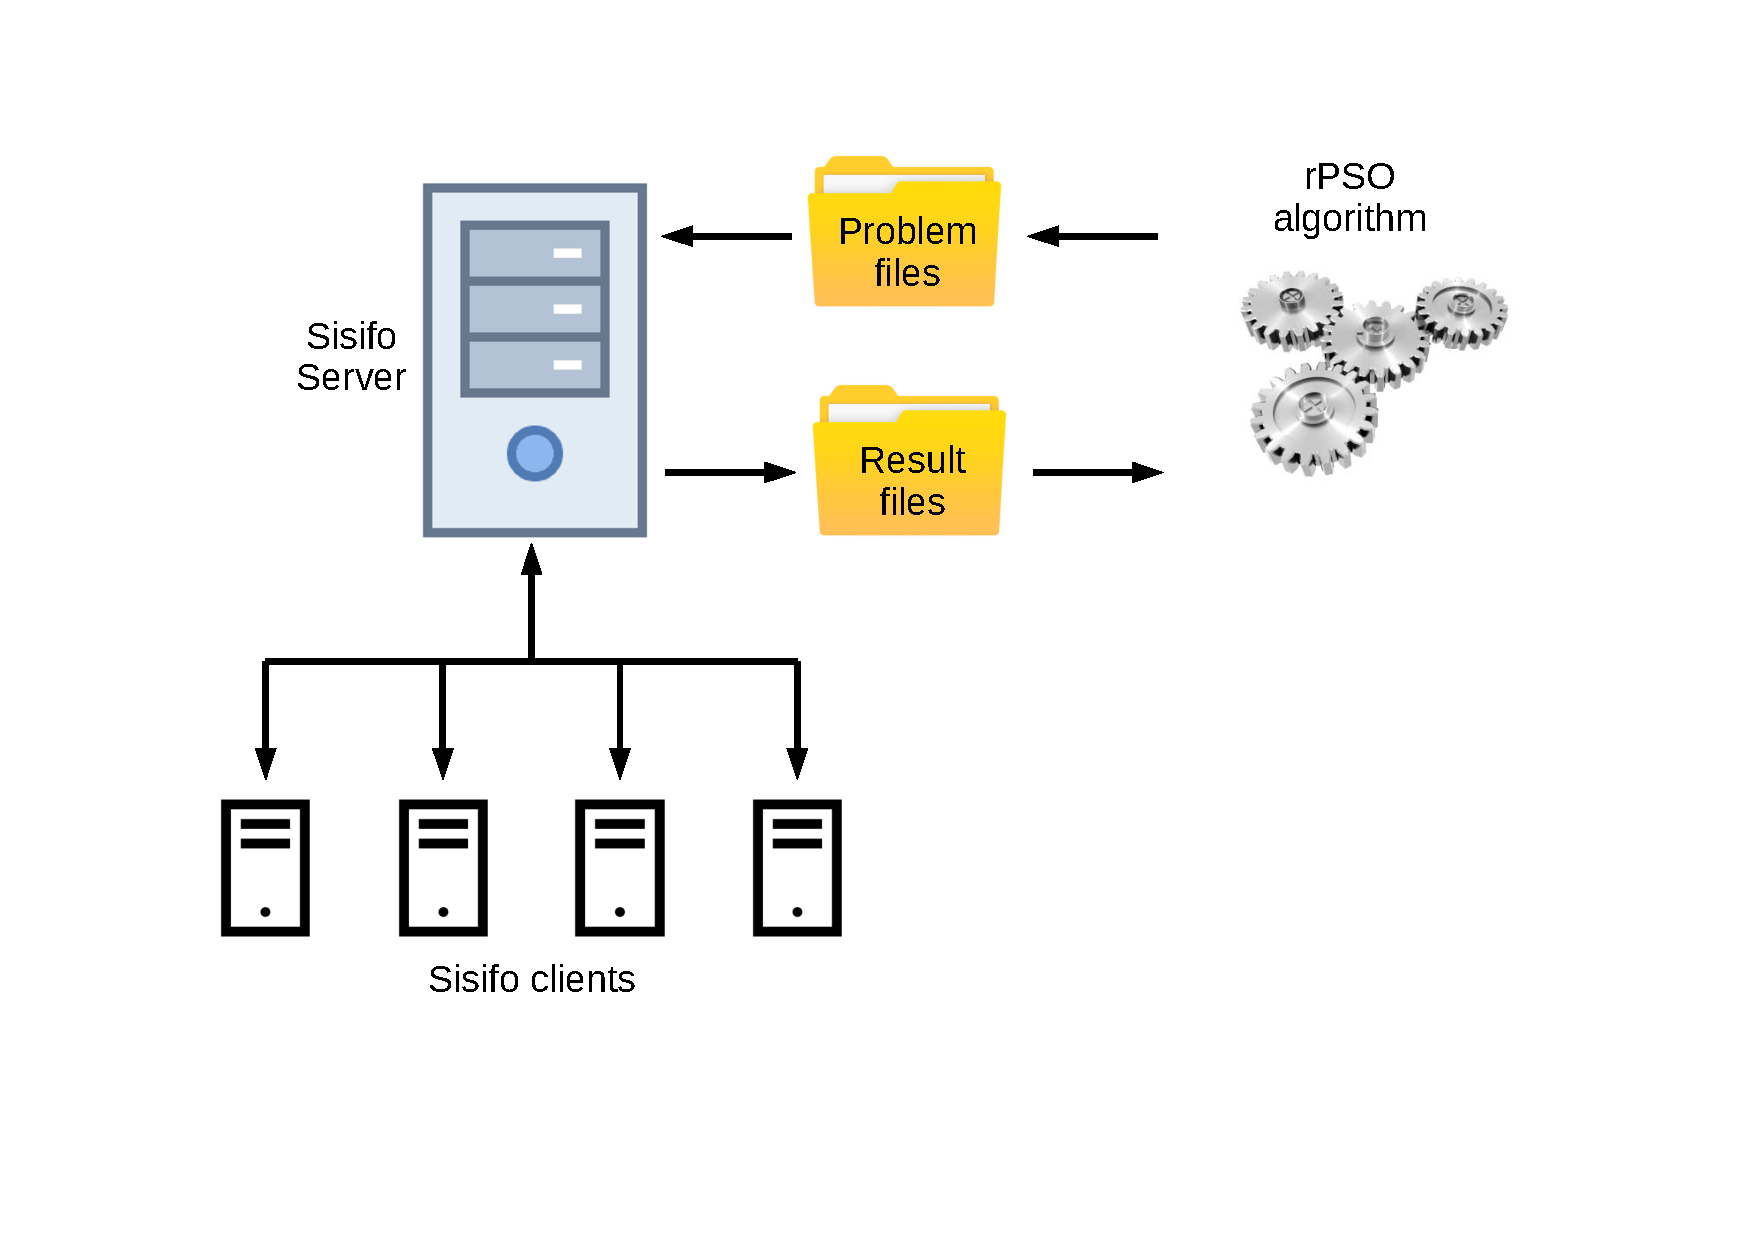
\includegraphics[width=0.6\linewidth]{IMGs/1.-Calibrado/Esquema_2.pdf}
	\caption{Introduction of the asynchronous rPSO algorithm in the Sisifo environment. rPSO manages the generation of new problems and put them in the \textit{Problem files} folder and the reading and processing of the solution files located in the \textit{Result  files} folder.}
	\label{rPSO.python}
\end{figure}

When the procedure starts, with the initialization of the particles (Step 1) we create their corresponding problem files in the \textit{Problem files} folder. The \textit{Sisifo Server} detects new problem files and distribute them among idle \textit{Sisifo Clients}. These clients carry out the realizations. When a Sisifo client ends its task, a results file is generated and sent to the \textit{Sisifo Server} that drops it on the \textit{Result files} folder. Every time a new results file appears in the \textit{Results files} folder, the asynchronous rPSO, in Step 4, reads the data from the results file and calculates the fitness. Then, updates the velocity taking into account the current existing global best and its individual best particles (Step 2), updates the particle (Step 3) and with the new model parameters creates a new problem file in the \textit{Problem files} folder. And so on. 

\subsection{Fitness function and some features included in the rPSO}\label{sec:rPSO}
There are some features included in our version of the asynchronous rPSO algorithm that we have to describe. 

\begin{enumerate}
	\item In the Step 3, we include the possibility to discard the new particle and generate a new one randomly with $10\%$ probability. If it is not discarded, with $10\%$ probability we apply to the new particle a mutation.  
	\item The fitness evaluation is made as follows: 
	\begin{itemize}
		\item we start the model and after a warm-up time of $ 400 $ simulated months, we get a stabilization of the model output; 
		\item we take the model output from month $ 401 $ to $ 500 $ for the subpopulations in the data of Table \ref{datosConstruccion}, i.e., percentage of women HR- and LR-infected per group ages $18-29$ and $18-64$;  
		\item then, for each subpopulation, we calculate the maximum and the minimum of these portions of the model output and we see if these maximum and minimum are inside the corresponding data $95\%$ confidence interval;
		\item if this happens, the fitness is zero; 
		\item otherwise, the fitness is the sum of the distances from these maxima and minima to the corresponding $95\%$ confidence interval of the data.
	\end{itemize}
	
	\item The definition of the fitness function may provide the same fitness values for different particles. Therefore, we are going to store all the particles with the same best fitness and, in Step 2, we chose  $p_{global}^{best}$ randomly among the stored particles.	
	\item As we mentioned before, physicians around the world have published estimations of most of the model parameters \cite{Durex2002,elbasha2007model,Giuliano2011,Nyitray2015}. It is clear that we have to respect their estimation in our fitting procedure avoiding that some model parameters overpass the estimation intervals. Furthermore, finding model parameters in the range of the estimations, gives credibility to our model. Therefore, when a model parameter is less than $1\%$ closer to an extreme of the interval provided by the physician estimations, we discard this value and it is substituted by a random value inside the interval.  
\end{enumerate}

It is worth to note that the above points 1, 3 and 4 will allow us to explore extensively the whole space of parameters avoiding the accumulation of particles close to the borders. 

\begin{remark}\label{mo}
At this point, we want to remark that to evaluate the fitness function, we do not need the model output for all the subpopulations. Only is necessary the output corresponding to HR- and LR-infected women in the group ages $18-29$ and $18-64$. Then, when a realization is carried out, we retrieve and process from the results file the data corresponding to the above subpopulations from the month $401$ to $500$, write them in a row and this row is stored as the result of the realization to be used later. 

Also, in order to compare properly the model output row with the data, we build the data vector mean, percentile $2.5$ and percentile $97.5$, repeating $100$ times the $4$ values of each we have in the Table \ref{datosConstruccion} and write them in a row.
\end{remark}

\section{Selecting an optimal number of particles to calibrate the HPV large network computational model with rPSO}
As we have mentioned above, on previous implementations of the parallel rPSO, we realized that we can not affirm that \textit{the higher the number of particles, the better the quality of the solution}. Moreover, we also detected that, due to our asynchronous parallel implementation, sometimes the use of more processors does not mean lower execution times. We would need more experiments to detect the correct cause of the delays. However, in this case is more practical to investigate what is the optimal combination of particles to achieve the best quality with the lowest number of processors.

To perform this test, we are going to build HPV network models with $50,000$ nodes. We execute 5 repetitions of the same problem with different number of particles. Times are shown in seconds. Thus, the question is, what is the quality of the solutions for different number of particles? Table \ref{tab.color} shows relevant information regarding the quality of the solutions for different number of particles and 5 executions of each configuration. Each execution carried out 1200 particle evaluations. We measure the quality of the solutions on Table \ref{tab.color} by counting the number of fitness values equal to zero in the 5 executions (\textit{Total \# 0s}) and on average (\textit{Avg \#0s}). In addition, we also recorded the iteration at which the first zero appear on average (\textit{Avg  First}), from the last population of particles Fitness of the best, worst and average, averaged over 5 executions (\textit{Best at end}, \textit{Worst at end} and \textit{Avg at end}). And regarding executions time we show on Table  \ref{tab.color} information about the average total execution time for 1200 evaluations (\textit{Total Time}), the  worst execution time for one particle (\textit{Worst $t$}) and the best execution time for one particle (\textit{Best $t$}). Red color indicates the worst configuration, bold letters indicate the best and blue color the second best configuration.

\begin{table}[h]
	\centering
	\tiny \begin{tabular}{cccccccccc}
		
		\hline
		\cellcolor[HTML]{C0C0C0} 
		\#       & 
		Total  & 
		Avg    & 
		Avg    & 
		Best   & 
		Worst & 
		Avg    & 
		Total  &
		          &
		           \\
		
		\cellcolor[HTML]{C0C0C0} 
		particles &
		\#0s       &
		\#0s       &
		First       &
		at end    &
		at end    &
		at end    &
		Time      &
		Worst $t$ &
		Best $t$    \\ 
		
		\hline
		\cellcolor[HTML]{C0C0C0}
		25      & 
		18       &
		{\color[HTML]{3166FF} 3.60} & 
		\textbf{531.00}                & 
		\textbf{0.015486}            & 
		\textbf{0.429090}           & 
		\textbf{0.122573}            & 
		8422.00                         & 
		\textbf{148.60}              & 
		\textbf{107.00}               \\
		
		\cellcolor[HTML]{C0C0C0}30          & 
		\textbf{28}           & 
		\textbf{5.60}        & 
		{\color[HTML]{3166FF} 594.00}  & 
		0.003785 & 
		{\color[HTML]{3166FF} 0.445587} & 
		{\color[HTML]{3166FF} 0.131193} & 
		\textbf{6908.00}                & 
		{\color[HTML]{3166FF} 186.60}  & 
		{\color[HTML]{3166FF} 112.00} \\
		
		\cellcolor[HTML]{C0C0C0}35          & 
		8             & 
		1.60                        & 
		834.80                         & 
		{\color[HTML]{3166FF} 0.010211 }    & 
		0.576688                        & 
		0.149215                        & 
		{\color[HTML]{3166FF} 7105.00}  & 
		250.60                         & 
		119.60                        \\
		
		\cellcolor[HTML]{C0C0C0}40          & 
		16            & 
		3.20                        & 
		692.80                         & 
		0.003332                        & 
		0.524417                        & 
		0.132628                        & 
		8808.60                         & 
		389.40                         & 
		144.60                        \\
		
		\cellcolor[HTML]{C0C0C0}45          & 
		14            & 
		2.80                        & 
		790.40                         & 
		0.006458                        & 
		0.639775                        & 
		{\color[HTML]{FE0000} 0.149670} & 
		10004.00                        & 
		502.00                         & 
		177.20                        \\
		
		\cellcolor[HTML]{C0C0C0}50          & 
		11            & 
		2.20                        & 
		796.00                         & 
		0.005168 & 
		{\color[HTML]{FE0000} 0.658020} & 
		0.139089                        & 
		11124.40                        & 
		648.40                         & 
		220.00                        \\
		
		\cellcolor[HTML]{C0C0C0}55          & 
		2             & 
		{\color[HTML]{FE0000} 0.40} & 
		{\color[HTML]{FE0000} 1171.20} & 
		0.004330                        & 
		0.518894                        & 
		0.137088                        & 
		11905.80                        & 
		775.00                         & 
		207.40                        \\
		
		\cellcolor[HTML]{C0C0C0}60          & 
		12            & 
		2.40                        & 
		765.00                         & 
		{\color[HTML]{FE0000} 0.002153}                        & 
		0.546259                        & 
		0.132464                        & 
		13787.80                        & 
		857.00                         & 
		245.40                        \\
		
		\cellcolor[HTML]{C0C0C0}64          & 
		5             & 
		1.00                        & 
		985.40                         & 
		0.002763                        & 
		0.551228                        & 
		0.140977                        & 
		{\color[HTML]{FE0000} 18770.00} & 
		{\color[HTML]{FE0000} 1041.20} & 
		{\color[HTML]{FE0000} 379.20} \\ 
		
		\hline
	\end{tabular}
	\caption{Analysis of the quality and execution times of different rPSO configurations. Results of 1200 evaluations for different number of particles on the rPSO process (\# Part.).}
	\label{tab.color}
\end{table}

As we can see, 25 and 30 particles are the preferred configurations, since we obtained the higher number of zeros in total and on average and the lower executions times. Since the results of 25 particles shows a very good execution with 7 zeros and also a very good execution time, we can conclude that the configuration with 30 particles should be selected bearing in mind both quality and execution time. Results on total number of 0s and total time were statically significant with $p$ value of $0.1$ after an ANOVA analysis.

\section{Improving the exploration of the rPSO}
As we explained on Section \ref{sec:rPSO}, we established a procedure respect to the intervals for the parameter values proposed by physicians. Some algorithms such as differential evolution \cite{storn1997differential} allows to overpass these limits in the search of a good combination of parameters. However, this is not a good idea when implementing our parallel rPSO. First, remember that our parallel version is asynchronous and the updating of the particles is made once every particle is evaluated. Allowing particles with parameters close to the limits trespass them, could lead to a chaotic search. Second, parameters out the defined bounds have not a medical meaning. Therefore, when a model parameter is less than $1\%$ closer to an extreme of the interval provided by the  estimations, we discard this value and it is substituted by a random value inside the interval. This allows also to made a deeper and more efficient exploration of the search space.

Figure \ref{Ctg} shows the exploration performed in some of the parameters of the model (duration and contagion parameters). Figures represent the values of the parameters during the 20 executions of rPSO algorithm with 500 realizations each one. X axis represents the realization number and Y axis the value of each parameter. We can see that we find points on most of the search space.

\begin{figure}[!h]
\begin{center}	
\begin{tabular}{cc}
	Time of clearance of        & Time of clearance of \\
	HPV high risk               & HPV low risk          \\
	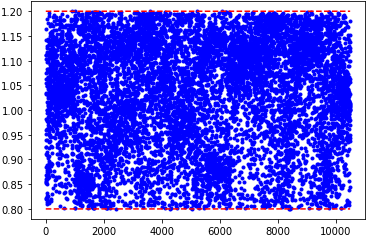
\includegraphics[width=0.45\textwidth]{IMGs/1.-Calibrado/Dura_HR_H.png} & 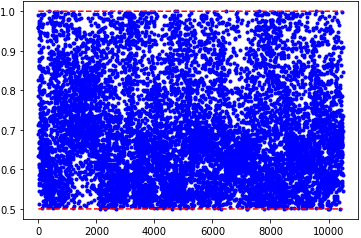
\includegraphics[width=0.45\textwidth]{IMGs/1.-Calibrado/Dura_LR_H.png} \\ 
	\\
	Women transmission probability & Men transmission probability \\
	of HPV low risk                & of HPV high risk             \\
	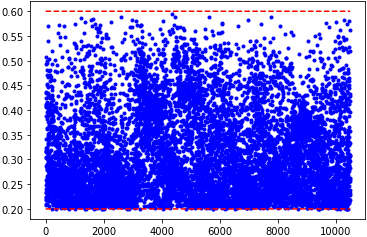
\includegraphics[width=0.45\textwidth]{IMGs/1.-Calibrado/Ctg_M_LR.png} & 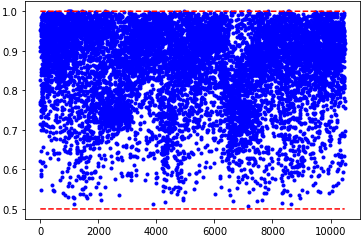
\includegraphics[width=0.45\textwidth]{IMGs/1.-Calibrado/Ctg_H_HR.png}  
\end{tabular}
\caption{Upper figures: Time of clearance of HPV high risk and low risk, both for men and women. Lower figures: on the left, probability to transmit low risk HPV if the infected is a woman; on the right, probability to transmit high risk HPV if the infected is a man. Red dashed lines correspond to the bounds of each parameter. We can see that most of the search space is explored in all the cases.} 
\label{Ctg}
\end{center}
\end{figure}

\section{Calibrating the model}
Now, we are going to perform the calibration. We use the Sisifo environment with the modified rPSO and 30 particles. The HPV network models will have $100,000$ nodes. In order to guarantee the reproducibility of the realizations, we are going to include in the problem files the seeds for the generation of the random numbers during the calibration process.

We assume that, initially, data of prevalence from Table \ref{datosConstruccion} are not only for women but also for men. Then, we label women and men as infected randomly following these prevalence data. Also, we start executing the realization and the first $400$ months are used as a warm-up period to stabilize the distribution of infected men and women. Thus, the goal is to calibrate the model parameters in such a way that the model output related to women HR and LR prevalence minimize the fitting function defined in Section \ref{sec:rPSO}.

We have performed 20 different calibrations using rPSO, each one with around $500$ realizations and $30$ particles. A total of $10,100$ realizations of the model were performed with an equivalent sequential total computation time of $161$ days. Computer time, however, is highly reduced as we can see in Figure \ref{histogram} due to the benefits provided by Sisifo distributed architecture.

\begin{figure}[!h]
	\centering
	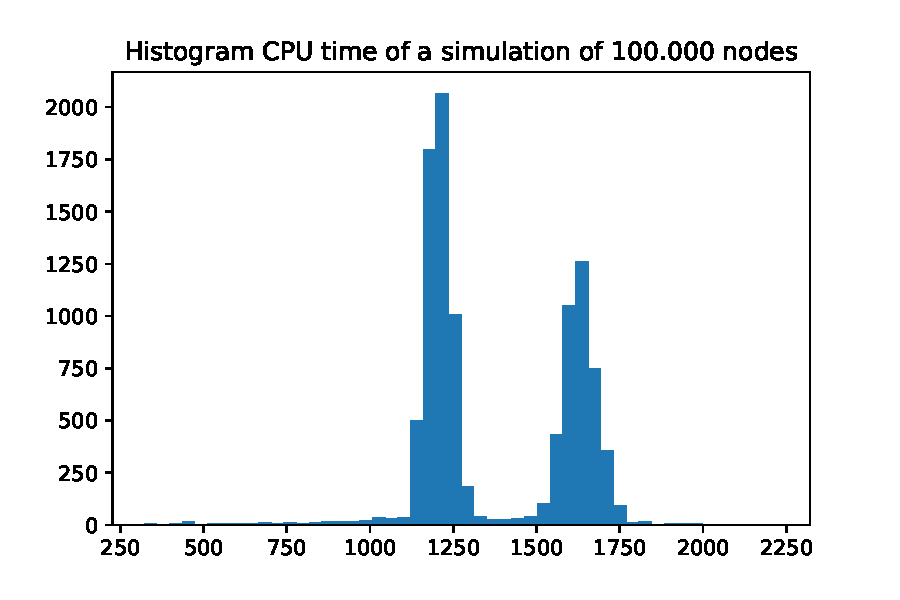
\includegraphics[width=0.6\linewidth]{IMGs/1.-Calibrado/Hist_CPU_time.pdf}
	\caption{Histogram of the computation time of each one of the $10,100$ realizations of the model using networks of $100,000$ nodes. The average time is $1374.5$ seconds, around $23$ minutes.}
	\label{histogram}
\end{figure}

\section{Selecting the 30 realizations that best capture the data uncertainty}
Our goal, now, is to find a procedure to select $30$ among the $10,100$ realizations of the model in such a way that the means and the 95\% confidence intervals of these $30$ realizations be as much close as possible of the corresponding means and the 95\% confidence intervals of the data in Table \ref{datosConstruccion}. We decided to select $30$ because as we saw in Table \ref{tab.color}, the total computation time is the best for $30$ particles executing in parallel in the Sandy Bridge computers.

Nevertheless, it would be interesting to reduce the number of eligible realizations to much less than $10,100$. In Figure \ref{Error_0} we can see the $100$ realizations with error less than $0.01$, that is, the realizations that almost lie inside the 95\% confidence intervals of the data, represented by the blue horizontal dashed lines. 

\begin{figure}[h!]
	\centering
	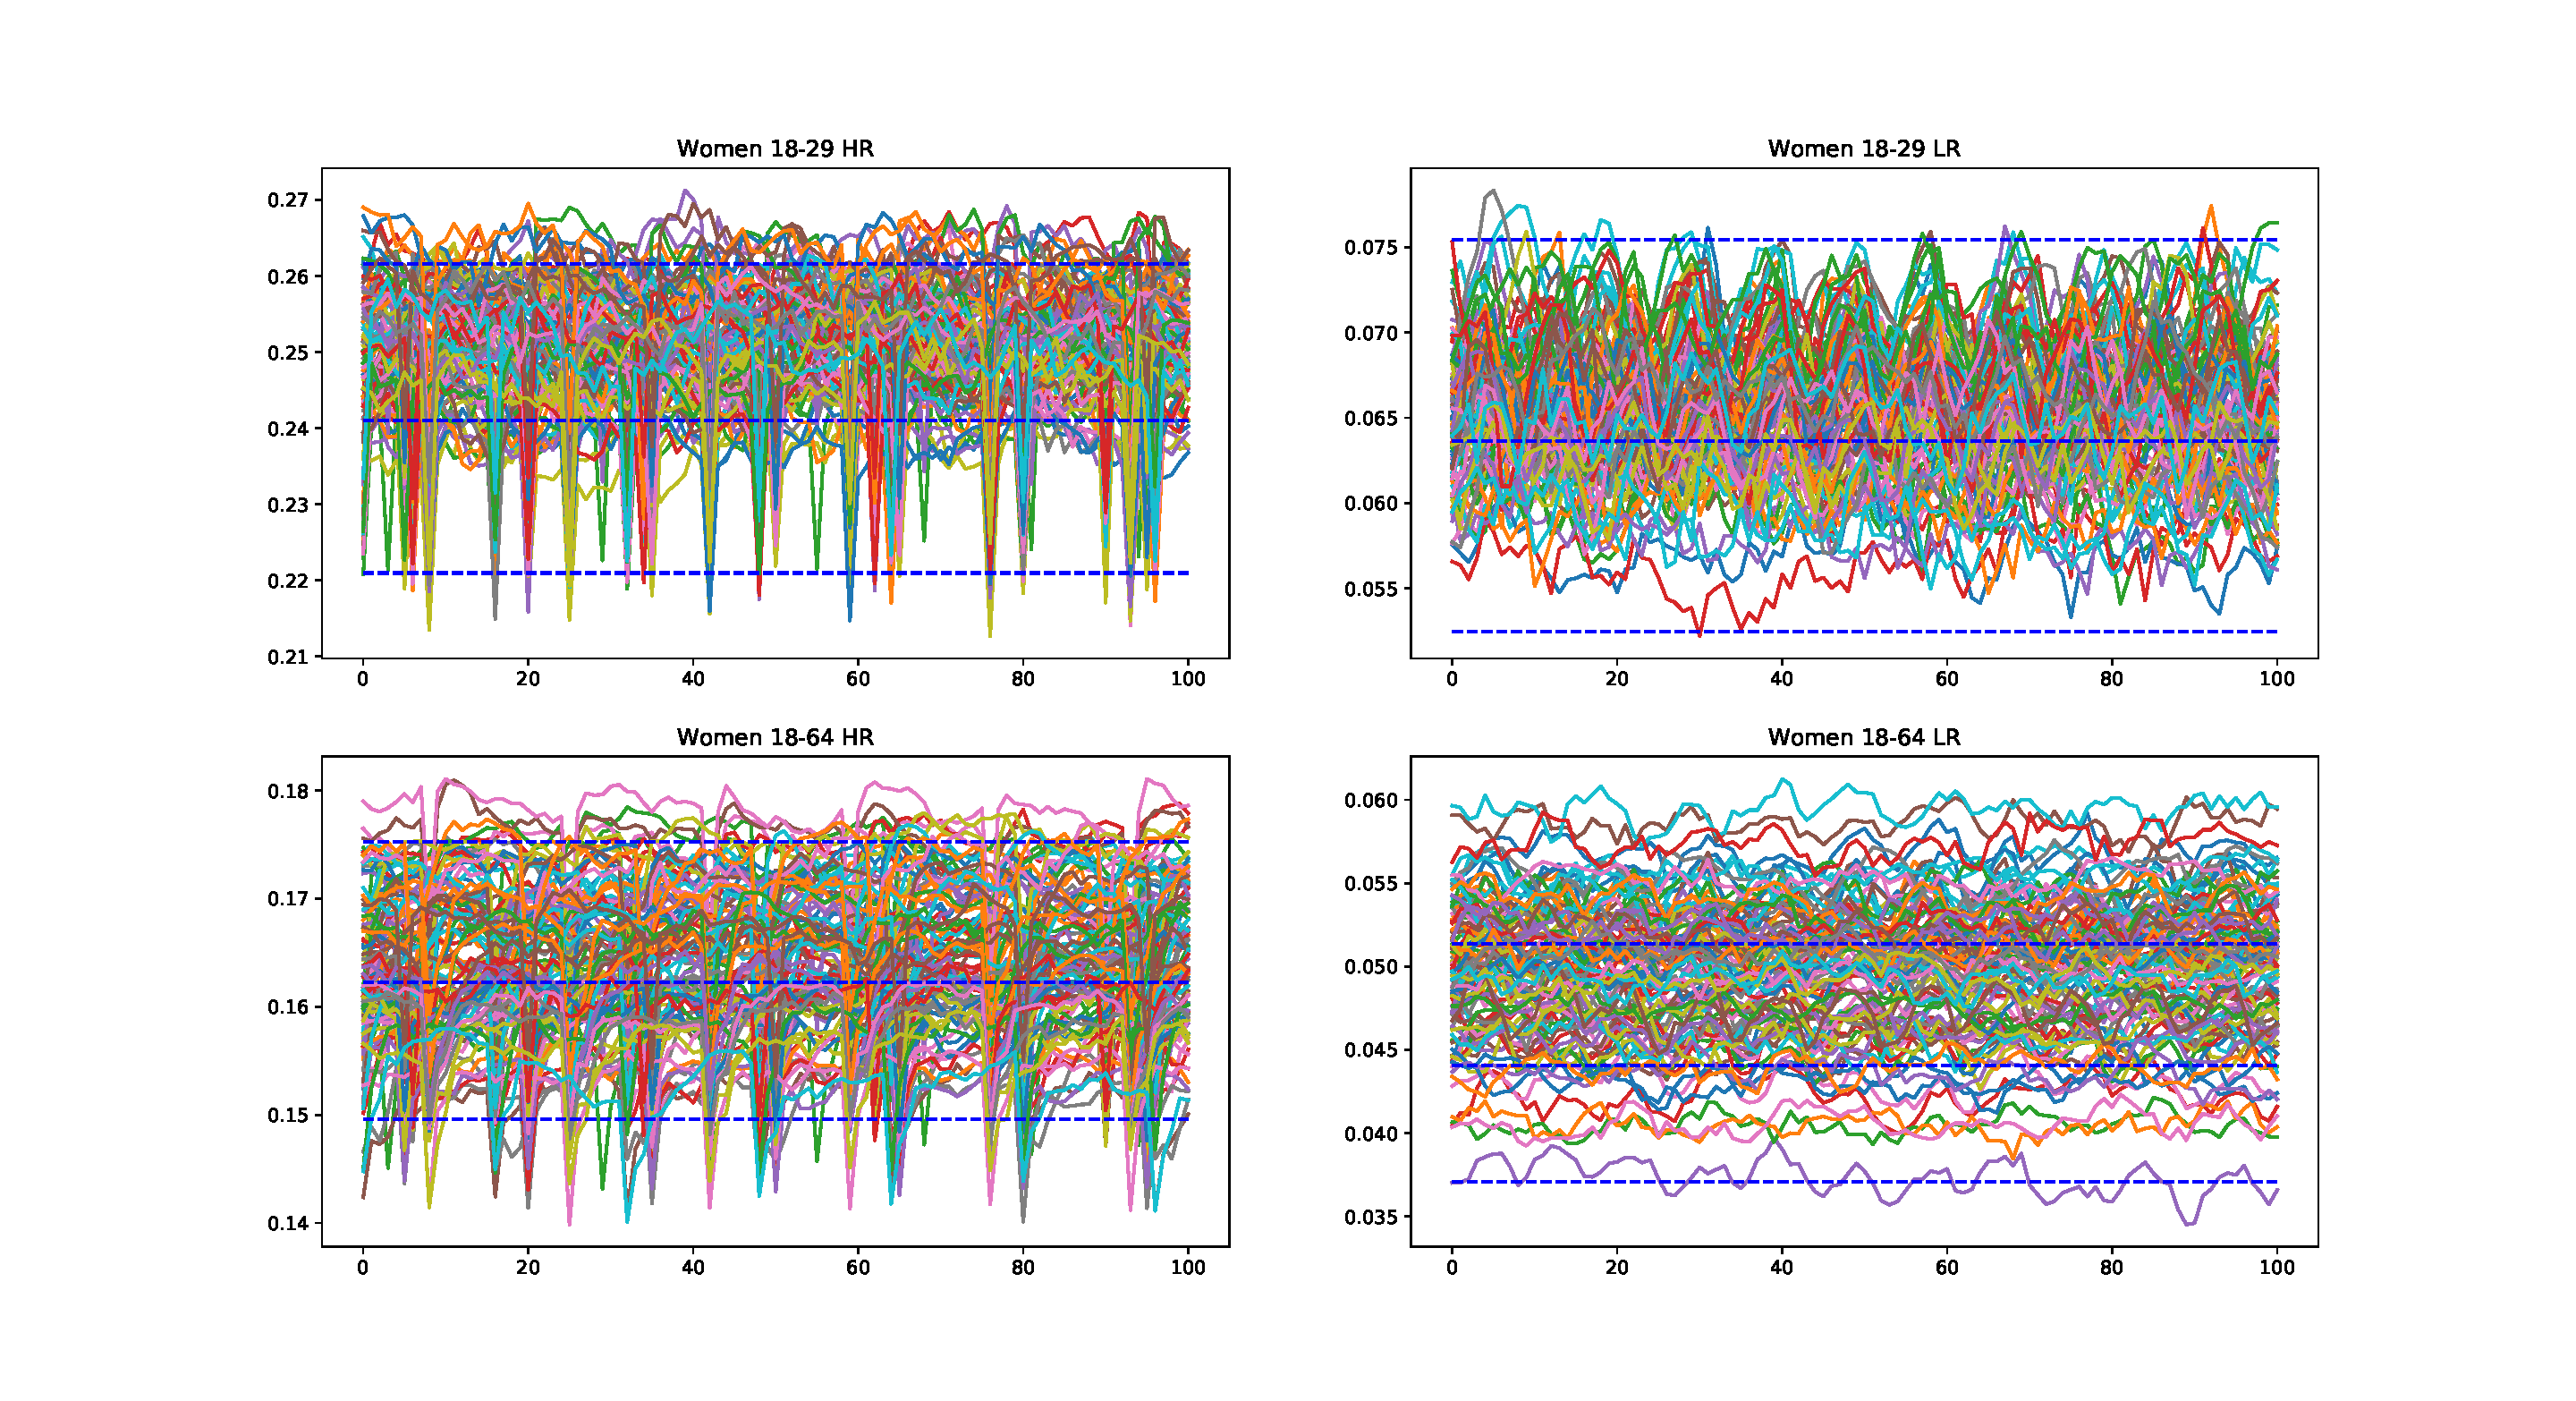
\includegraphics[width=\linewidth]{IMGs/1.-Calibrado/Error_001.pdf}
	\caption{Drawing of the $100$ model realizations with error less than $0.01$ from month 400 to 499. }
	\label{Error_0}
\end{figure}

If we select $30$ among these $100$, it is clear that some percentiles of the model will be far from the corresponding percentiles of the data, for instance, the lower parts of the left figures. Therefore, we need to consider realizations with errors greater than $0.01$ without forgetting the objective to reduce the number of eligible realizations.  

Thus, we check the number of possible realizations depending on their error. Then, there are $2$ realizations with error $0$,  $100$ realizations with error less than $0.01$, $392$ with error less than $0.025$, $1282$ with error less than $0.05$ and $2607$ with error less than $0.075$. 
In Figure \ref{Error_003}, we draw the $1282$ model realizations of with error less than $0.05$. Note that the realizations cover completely the 95\% confidence intervals of the data. 

\begin{figure}[h!]
	\centering
	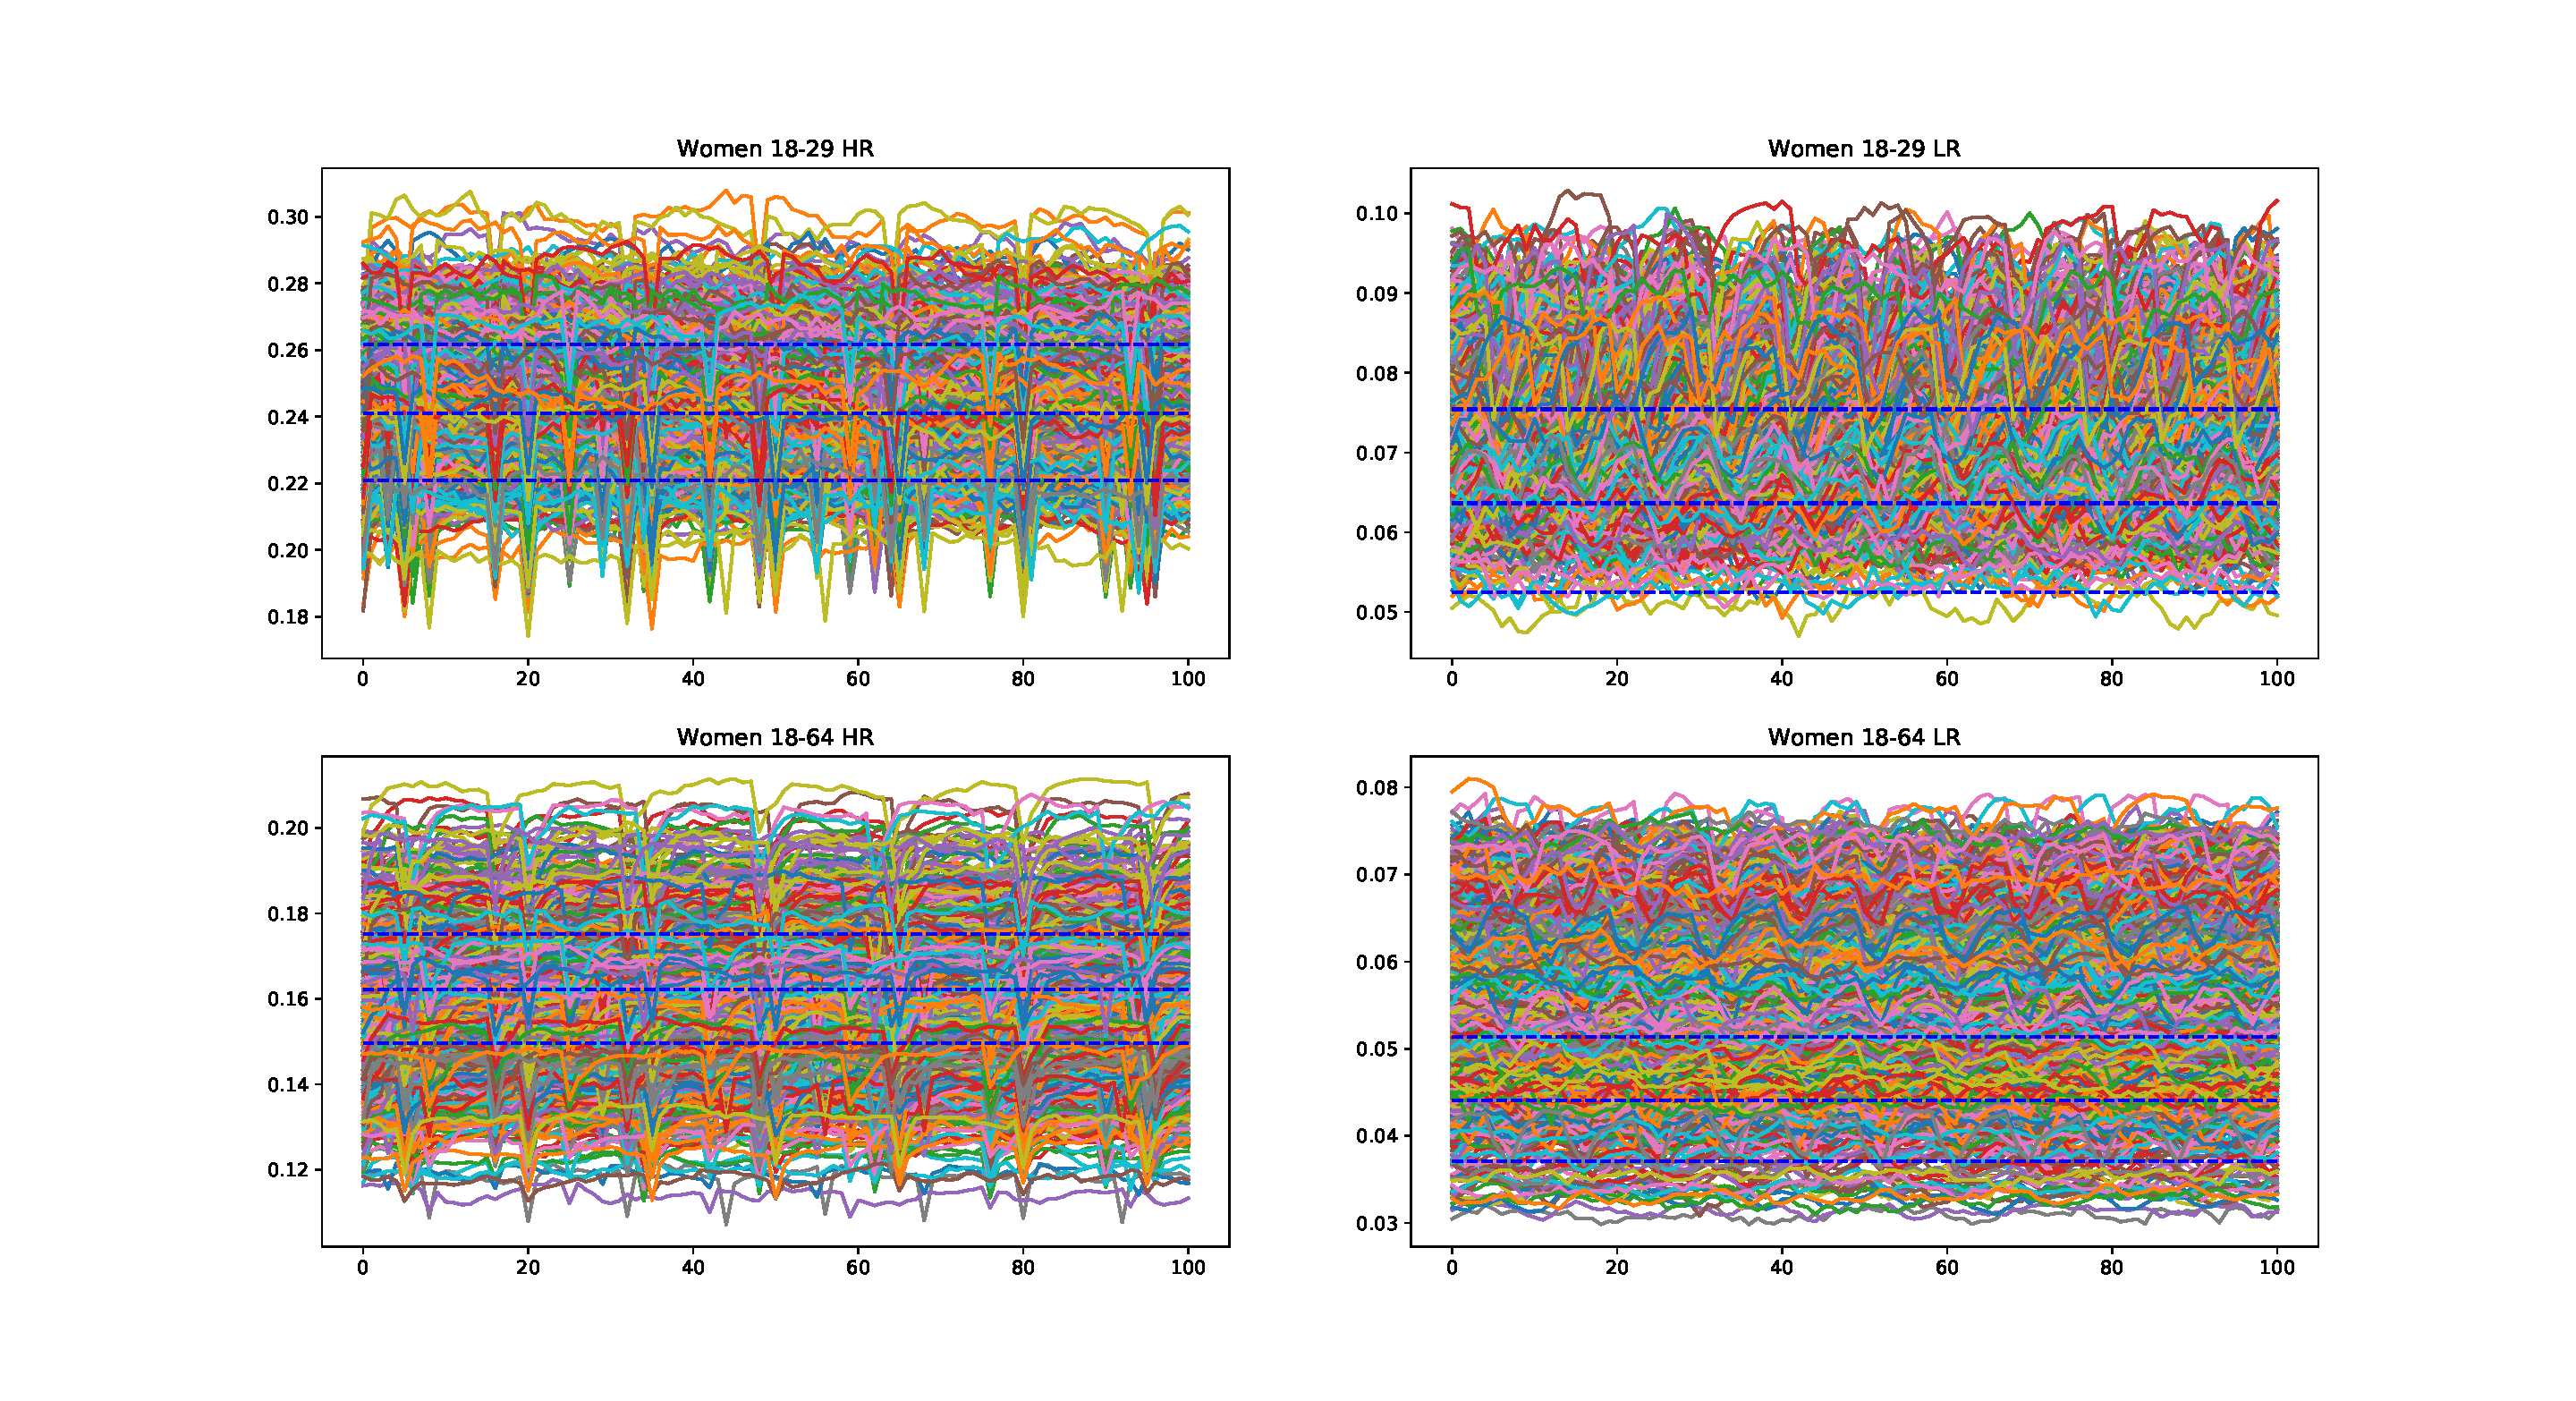
\includegraphics[width=\linewidth]{IMGs/1.-Calibrado/Error_005.pdf}
	\caption{Drawing of the $1282$ model realizations with error less than $0.05$ from month 400 to 499. These realizations cover the 95\% confidence intervals of the data, represented by the blue horizontal dashed lines.}
	\label{Error_003}
\end{figure}

In order to determine the \textit{best} $30$ realizations that capture the mean and the $95\%$ confidence intervals of the data in Table \ref{datosConstruccion}, we are going to introduce an adapted version of the rPSO algorithm before. Let $E$ be the realizations considered with $card(E)=M$ its number. For instance, for $E$ the set of realizations with error less than $0.01$, $M=100$. Also, for $E$ the set of realizations with error less that $0.05$, $M=1282$. Then $E(i)$ is the $i-th$ realization of the set $E$. We define the following fitness function $F$:

\begin{description}
	\item[INPUT:] Set of $30$ indexes $I=\{i_1,\ldots,i_{30} \}$, $1\leq i_j \leq M$, $j=1,\ldots, 30$.
	\item[Step 1.] Select the realizations $E(i_1),\ldots,E(i_{30})$ and calculate the mean, percentile $2.5$ and percentile $97.5$ of them.
	\item[Step 2.] Calculate the Root Mean Square Error (RMSE) of the difference between the mean, percentile $2.5$ and percentile $97.5$  of the $30$ realizations and the data (see Remark \ref{mo}), and sum them up. 
\end{description}

Now, the adapted version of rPSO to select the best $30$ realizations is

\begin{description}
	\item[Step 1.] Initialization.
	\begin{itemize}
		\item We have a set $E$ with $M$ realizations.
		\item Initialize $N$ index subsets $S_1,\ldots,S_N$ with $30$ elements of the set $\{1,\ldots,M\}$ (particles) chosen randomly without repetition.
		\item Evaluate the fitness of all the particles $F(S_1), \ldots, F(S_N)$.
		\item Define the individual best fitness as $S_i^{best} = S_i$, $i=1,\ldots,N$ and the global best fitness $S_{global}^{best}$ as the $S_i^{best}$ which fitness is the minimum.
	\end{itemize}
	\item[Step 2.] For $i=1,\ldots,N$, build the new set $P_i=S_i \cup S_i^{best} \cup S_{global}$, that is, joining the current particle, its individual best and the global best. After removing index repetitions, the new particle $S_i$ consists of a random selection without repetition of $30$ indexes of $P_i$.
	\item[Step 3.] Evaluate the fitness of all the new particles $F(S_1), \ldots, F(S_N)$.	
	\item[Step 4.] Update the individual best fitnesses $S_i^{best}$, $i=1,\ldots,N$ and  the global best fitness $S_{global}^{best}$. Go to Step 2. 
\end{description}

Here, we also consider $10\%$ of randomness and $10\%$ of mutation when updating new particles. In this case, mutation consists of changing some of the indexes in the current particle by other randomly chosen indexes, avoiding repetitions.

The above algorithm, in the tests we have executed, last around $20$ minutes for $1$ million of evaluations of the fitness function in the Sandy Bridge computer, returning accurate solutions.

We have performed executions for $30$, $40$, $50$ and $60$ particles, being $E$ the realization sets with errors less than $0.025$, $0.05$ and $0.075$. The lowest error has been $0.1166$ for the following realizations  

\begin{equation}
\begin{array}{c}
85, 109, 460, 474, 475, 476, 485, 493, 496, 497, 523, 531, \\
542, 543, 563, 600, 635, 637, 650, 687, 715, 729, 730, \\
842, 974, 987, 1058, 1060, 1080, 1238,	
\end{array}
\label{laselegidas}    
\end{equation}

among the $1282$ of the set of realizations with error less than $0.05$. In Figure \ref{fig:laselegidas} we draw the selected realizations and in Figure \ref{fig:ajuste95IC} we can see the graphical result of the calibration and how resemble the means and 95\% confidence intervals.  

\begin{figure}[h!]
	\centering
	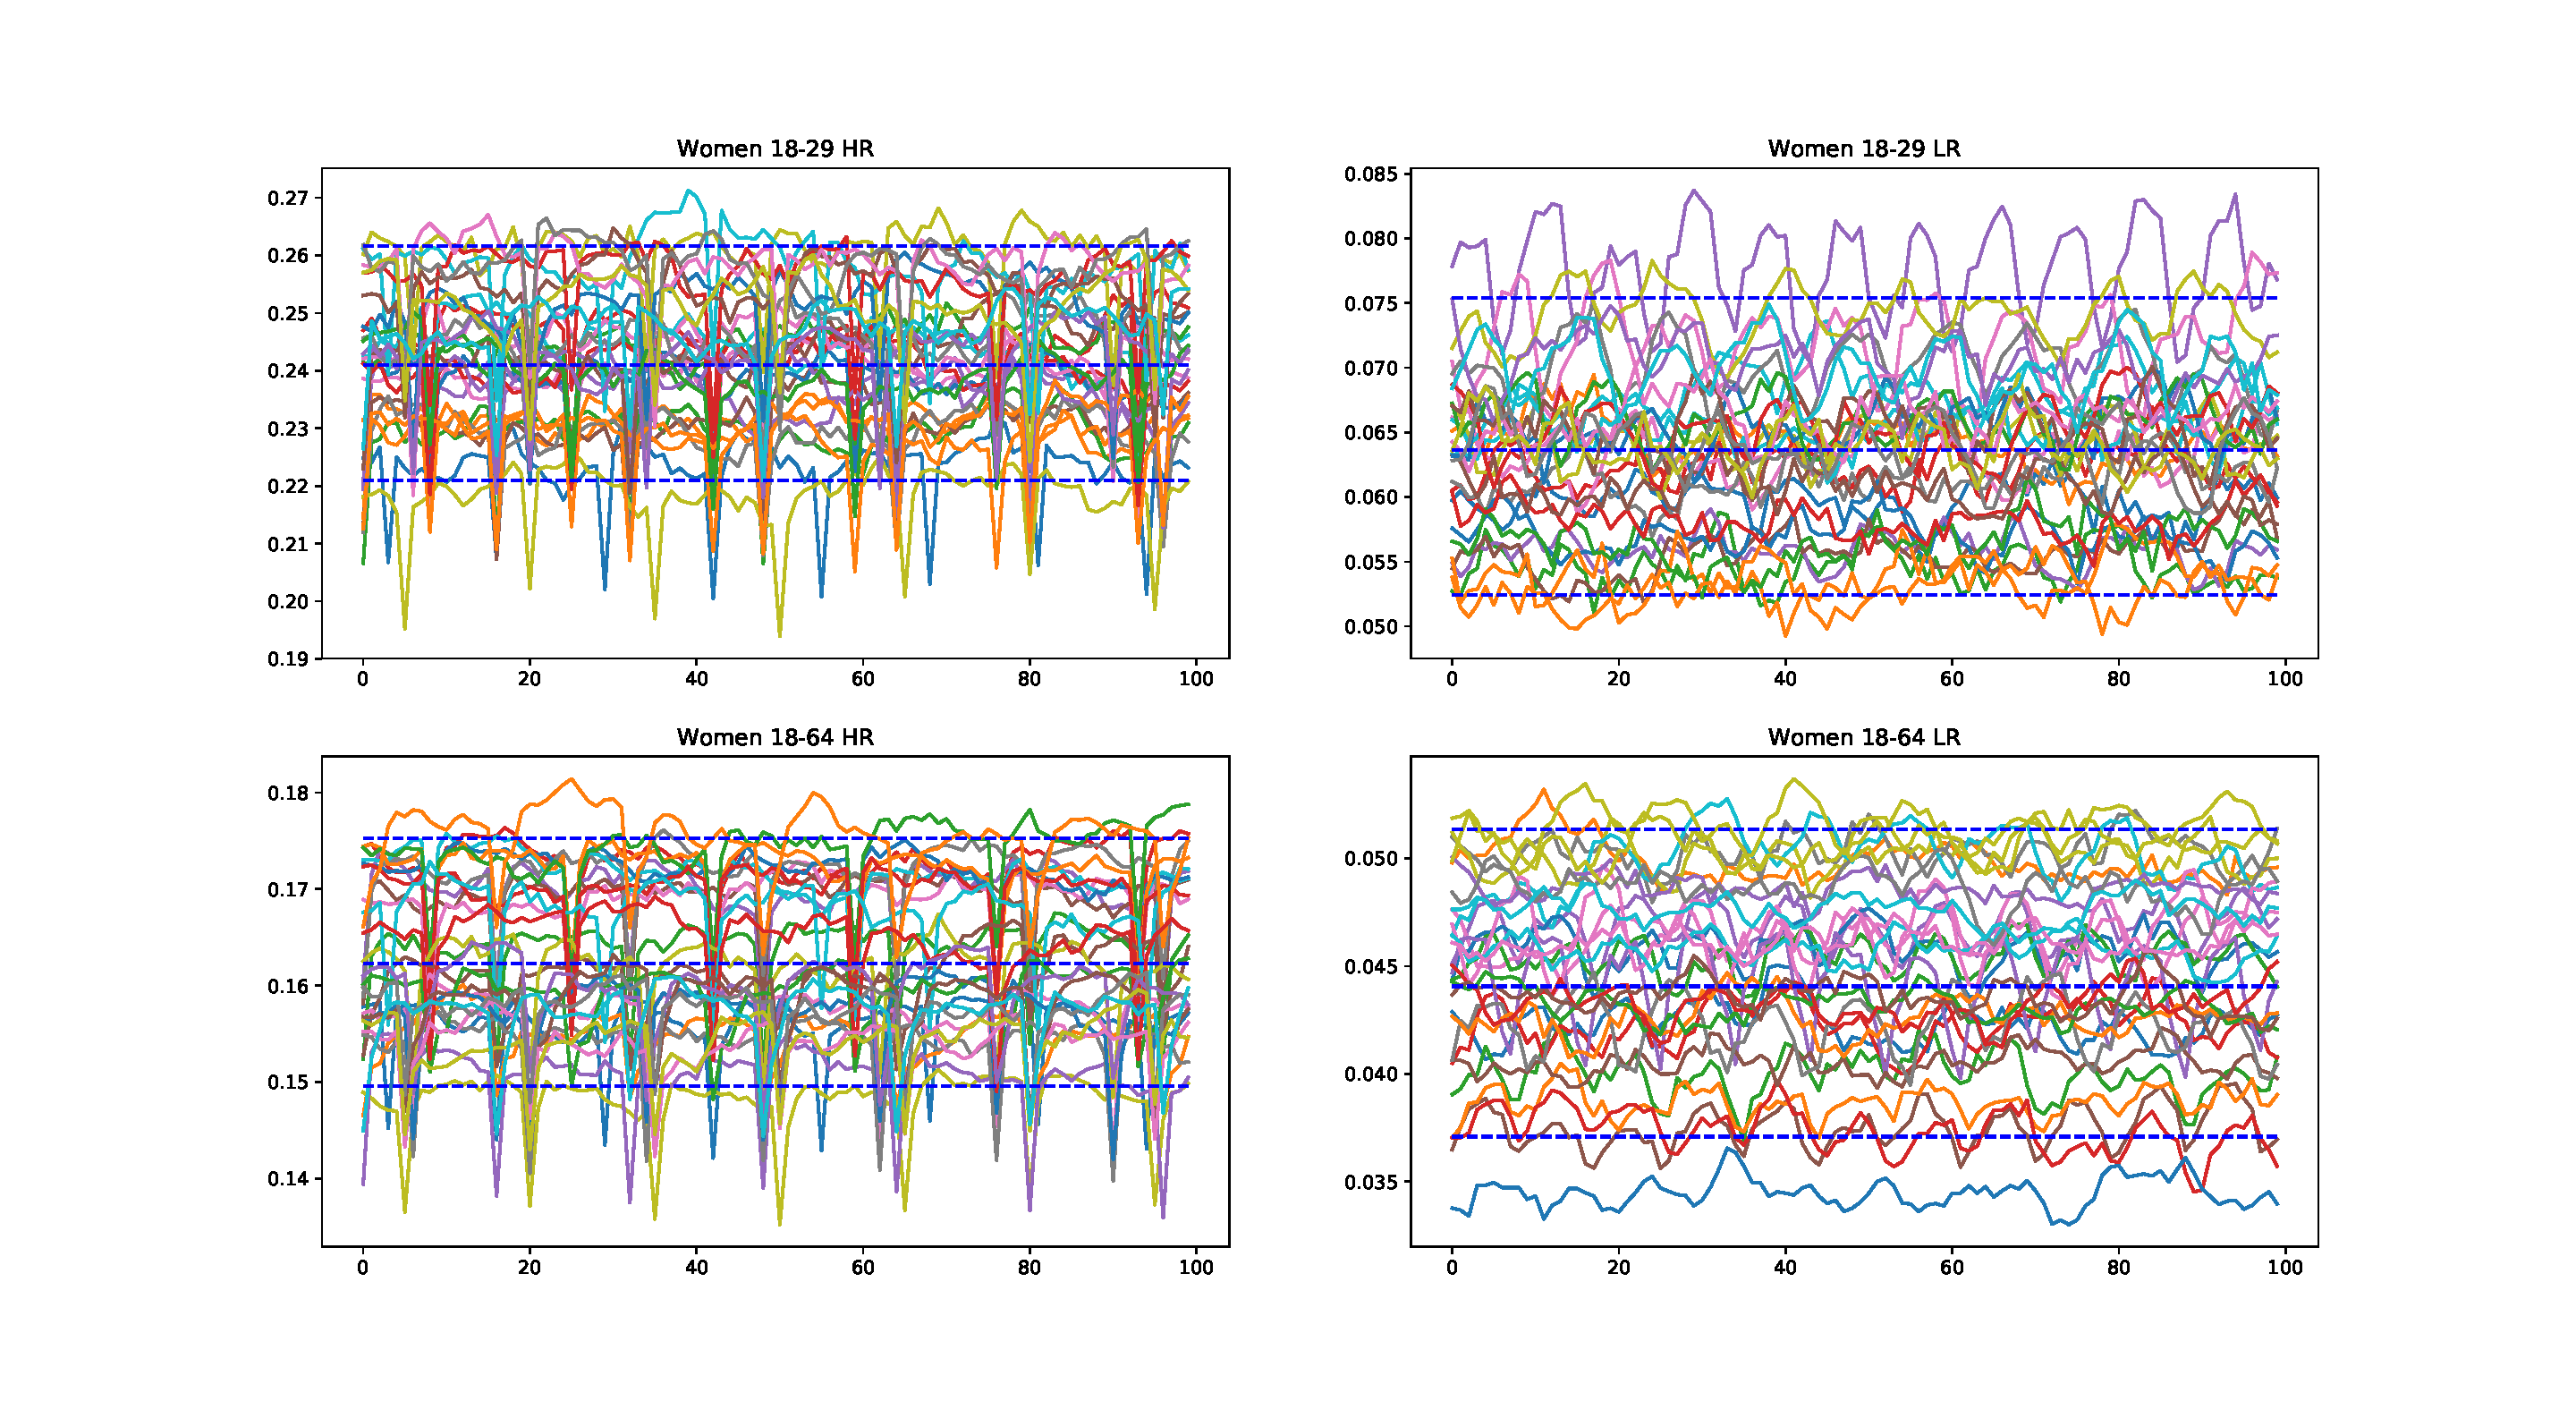
\includegraphics[width=\linewidth]{IMGs/1.-Calibrado/Selected.pdf}
	\caption{Drawing of the $30$ selected model realizations from month 400 to 499. These realizations are the ones whose means and 95\% confidence intervals resemble the most the data in Table \ref{datosConstruccion}, represented by the blue horizontal dashed lines.}
	\label{fig:laselegidas}
\end{figure}

\begin{figure}[h!]
	\centering
	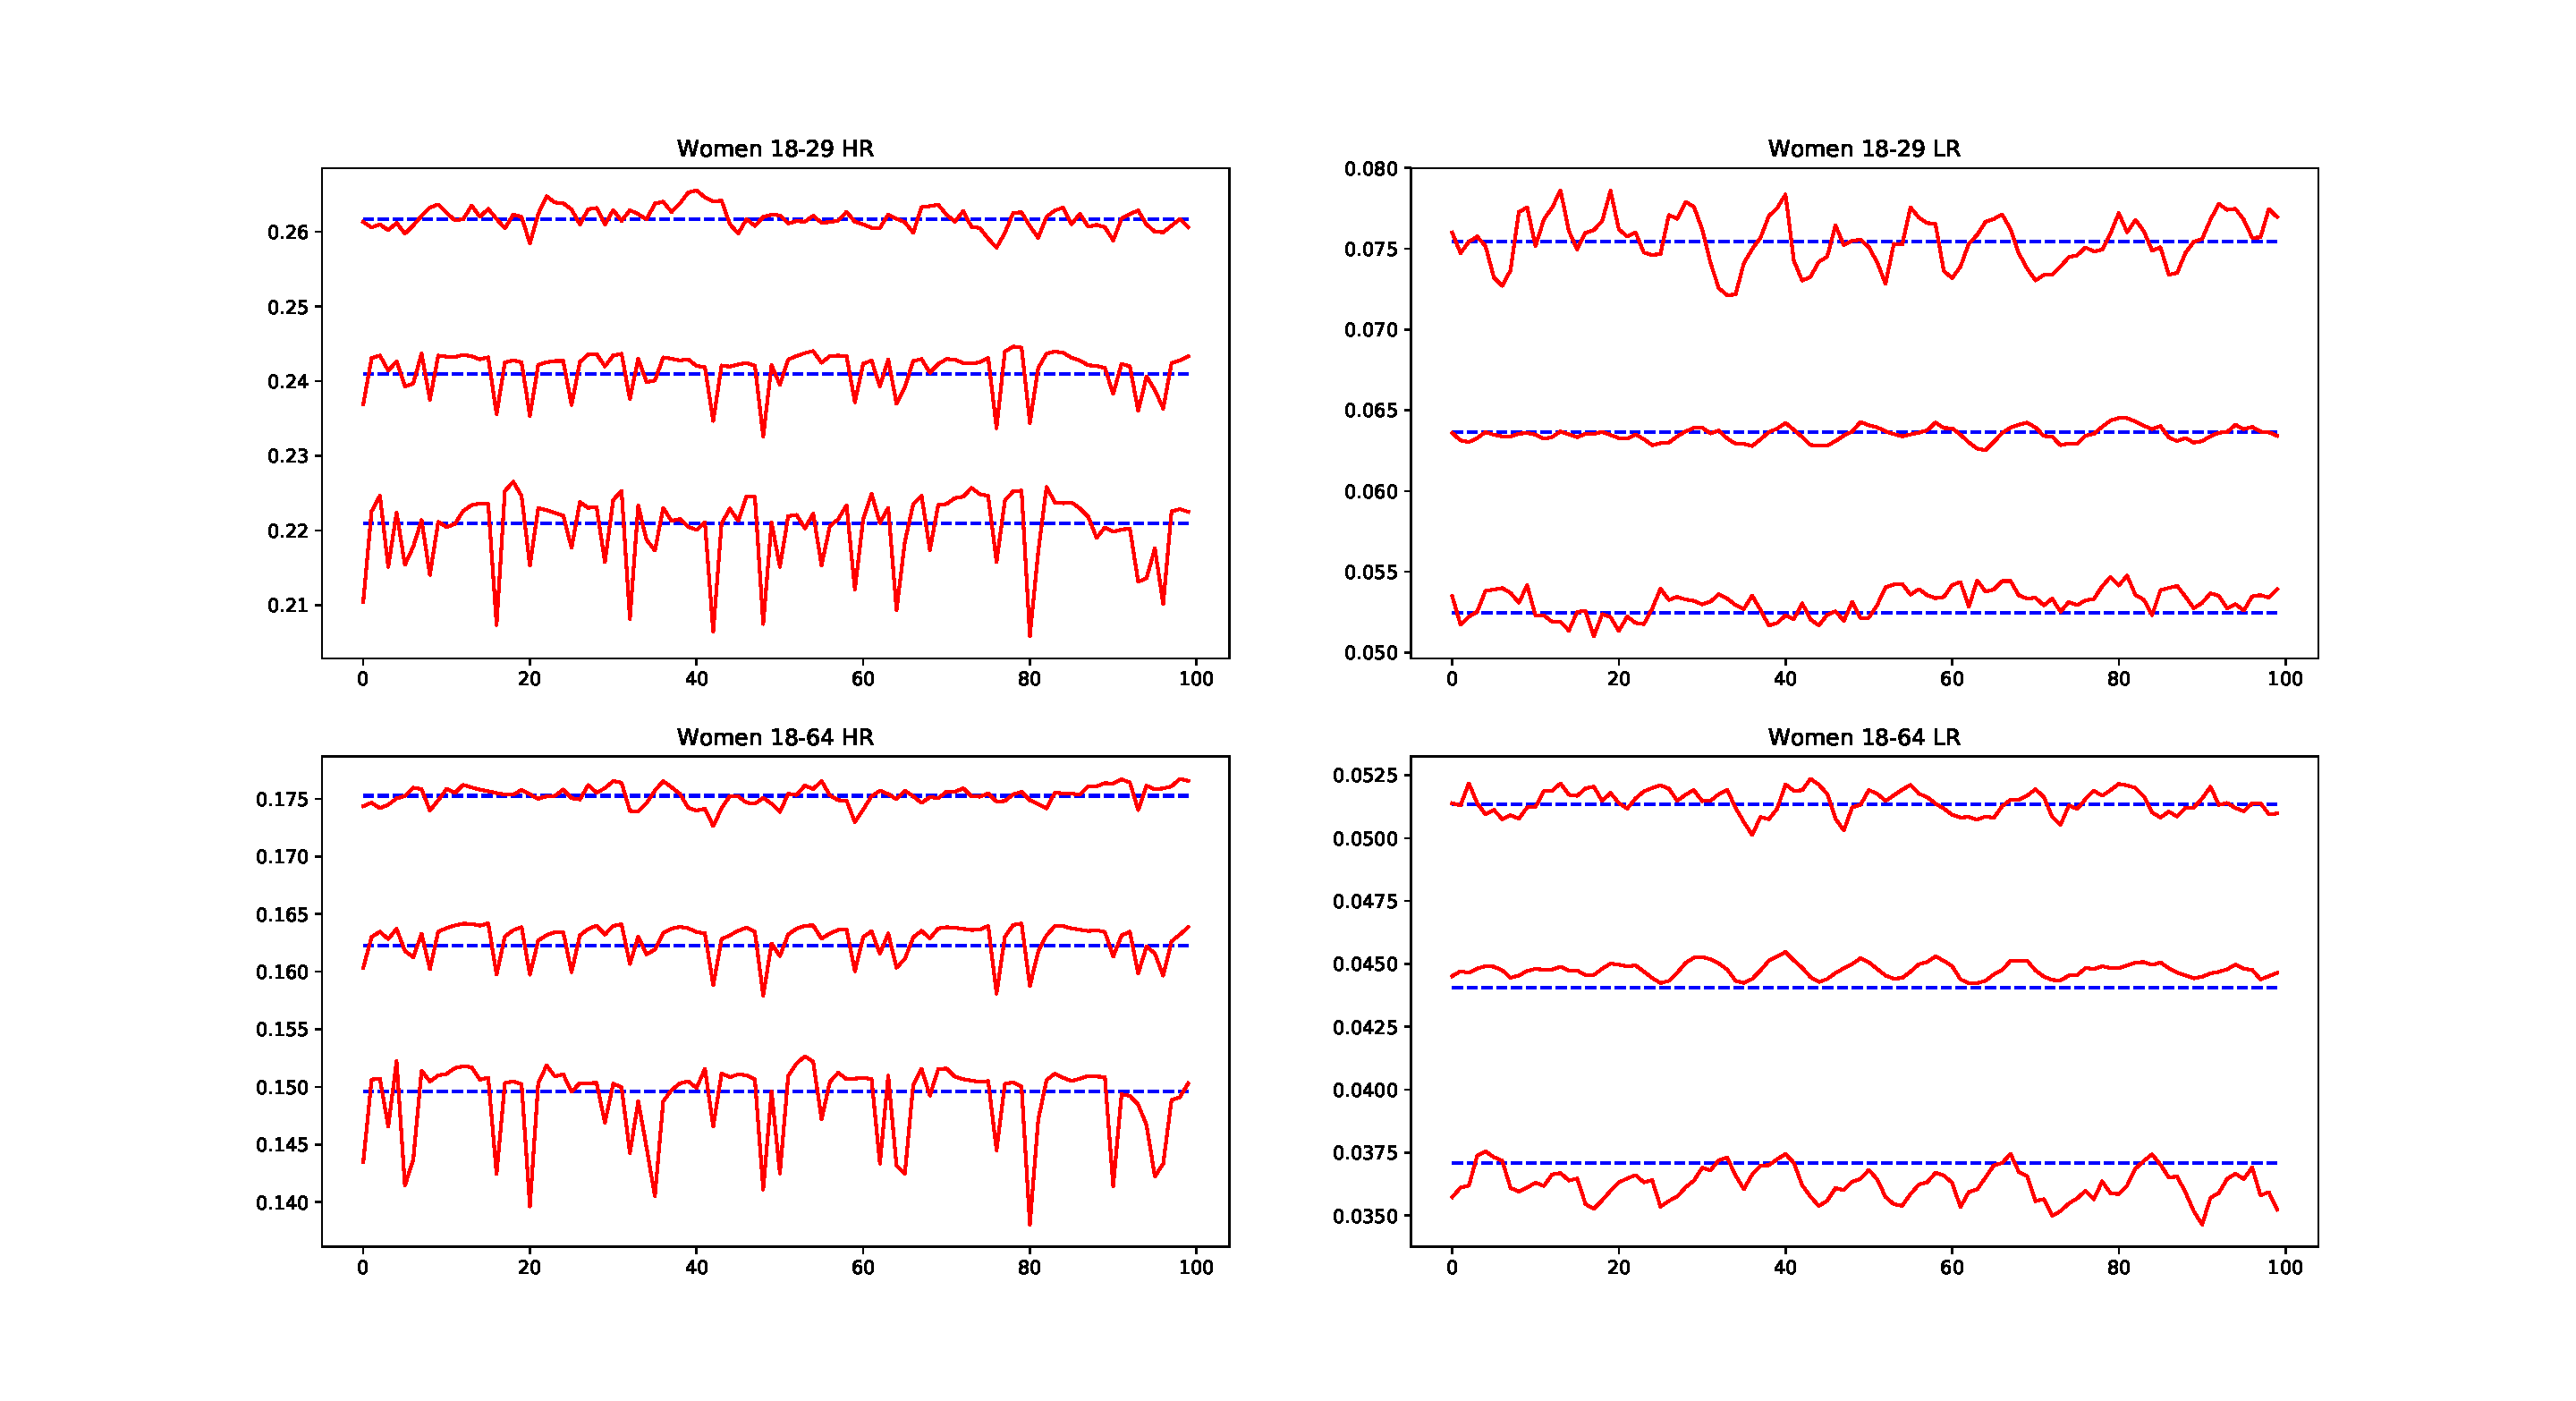
\includegraphics[width=\linewidth]{IMGs/1.-Calibrado/Ajuste_95IC.pdf}
	\caption{Means and 95\% confidence intervals of the $30$ selected realizations (in red) compared to the means and 95\% confidence intervals of the data (blue).}
	\label{fig:ajuste95IC}
\end{figure}

\section{Parameters returned by the calibration}

The mean and the 95\% confidence interval of the model parameters corresponding to the $30$ selected realizations from \eqref{laselegidas} are given in the Table \ref{table:laselegidas}. Note that the obtained model parameters are in accordance to the medical parameters appearing in the literature and collected in Section \ref{sec:modelo}. 

\begin{table}[!h]
	\begin{center}
		\begin{tabular}{|c|c|c|}
			\hline 
			Model parameter & Mean & $95\%$ confidence interval  \\ 
			\hline 
			Average LSP men & $8.63$ & $ [ 7.15 ,  9.86 ]$  \\ 
			Average time clearing HR HPV & $1.08$ &  $[ 0.88 ,  1.19 ]$ \\ 
			Average time clearing LR HPV &  $0.60$ & $ [ 0.52 ,  0.82 ]$\\ 
			Probability a woman transmits LR &  $0.23$ &  $[ 0.21 ,  0.29 ]$\\ 
			Probability a man transmits LR &  $0.28$ &  $[ 0.22 ,  0.37 ]$\\ 
			Probability a woman transmits HR &  $0.81$ & $[ 0.68 ,  0.95 ]$\\ 
			Probability a man transmits HR &  $0.91$ & $[ 0.74 ,  0.97 ]$ \\
			Frequency, 14-17 years old & $0.1098$ & $ [0.0485, 0.1542]$ \\
			Frequency, 18-29 years old & $0.0776$ & $[0.0568, 0.0981]$ \\
			Frequency, 30-39 years old & $0.0620$ & $[0.0024, 0.0935]$ \\
			Frequency, 40-65 years old & $0.0190$ & $[0.0046, 0.0553]$ \\
			\hline
		\end{tabular}
	\end{center} 	
	\caption{Mean and the 95\% confidence interval of the model parameters corresponding to the $30$ selected realizations from \eqref{laselegidas}. The last four parameters measures the global frequency of the sexual intercourses per age group. }
	\label{table:laselegidas}
\end{table}

The last four parameters in Table \ref{table:laselegidas}, as we defined in page \pageref{las_T}, are the global probabilities that determine if the existence of a LSP implies sexual intercourses in the current time step per age group $14-17$, $18-29$, $30-39$ and $40-65$. As we mentioned, these parameters measure the global frequency of the sexual intercourses per age group. We can see that, in average, the frequency in the older group is much less than the younger ones. In general, there is high uncertainty in these parameters.

%GM_hom 8.632401 , [ 7.155940749999999 ,  9.863097 ]
%T0 0.10987674333333333 , [ 0.04854902749999999 ,  0.15426519999999996 ]
%T1 0.07760148333333333 , [ 0.0568457325 ,  0.098102825 ]
%T2 0.06204759366666668 , [ 0.00249285925 ,  0.0935827675 ]
%T3 0.01900011266666667 , [ 0.00459073525 ,  0.055310677499999995 ]
%Dura_HR_H 1.0867896666666665 , [ 0.876574475 ,  1.1933470000000002 ]
%Dura_HR_M 1.0867896666666665 , [ 0.876574475 ,  1.1933470000000002 ]
%Dura_LR_H 0.6064539999999999 , [ 0.5235909000000001 ,  0.8265954999999999 ]
%Dura_LR_M 0.6064539999999999 , [ 0.5235909000000001 ,  0.8265954999999999 ]
%Ctg_M_LR 0.23338683333333335 , [ 0.20541835 ,  0.28724167500000003 ]
%Ctg_H_LR 0.28331856666666666 , [ 0.21561380000000002 ,  0.36796745 ]
%Ctg_M_HR 0.8150573666666665 , [ 0.67933955 ,  0.9515546500000001 ]
%Ctg_H_HR 0.9114978333333335 , [ 0.736503075 ,  0.968648425 ]

In the following, we are going to use the sets of parameters corresponding to the realizations \eqref{laselegidas} (and their corresponding seeds) to perform simulations. 

%Cap�tulo 4
% !TeX spellcheck = en_US
%\chapter{Making Dynamic Sexual Contacts Network and adding Vaccination Campaigns}\label{DinamicaYVacunacion}
\chapter{Including new features into the model: Dynamic LSP network and vaccination campaigns}\label{DinamicaYVacunacion}
%\section{Including new features into the model: Dynamic LSP network and vaccination campaigns}
\section{Introducing age and LSP dynamics into the LSP model}
The computational model presented so far is static, that is, once we have assigned the LSPs, they do not change over the time and the nodes do not increase their age. We modulate the possibility of a contagion introducing global probabilities that determine if the existence of a LSP implies sexual intercourses in a given time step per age group $14-17$, $18-29$, $30-39$ and $40-65$. Also, note that the available data about LSPs come from $2003$ and the data of prevalence appears in a study (CLEOPATRA \cite{castellsague2012prevalence}) conducted in $2007-2008$. The sexual behavior has changed in the last $10-15$ years and we would like to include it in our model in some way. Nevertheless, newer data about LSPs and prevalence in Spain are not available.

Thus, in order to introduce age and LSP assignation dynamics in a simple way, we are going to \textit{move} the available data over the time. Figure \ref{fig:dinam1} shows the constant age distribution that do not varies over the time.

\begin{figure}[h!]
	\centering
	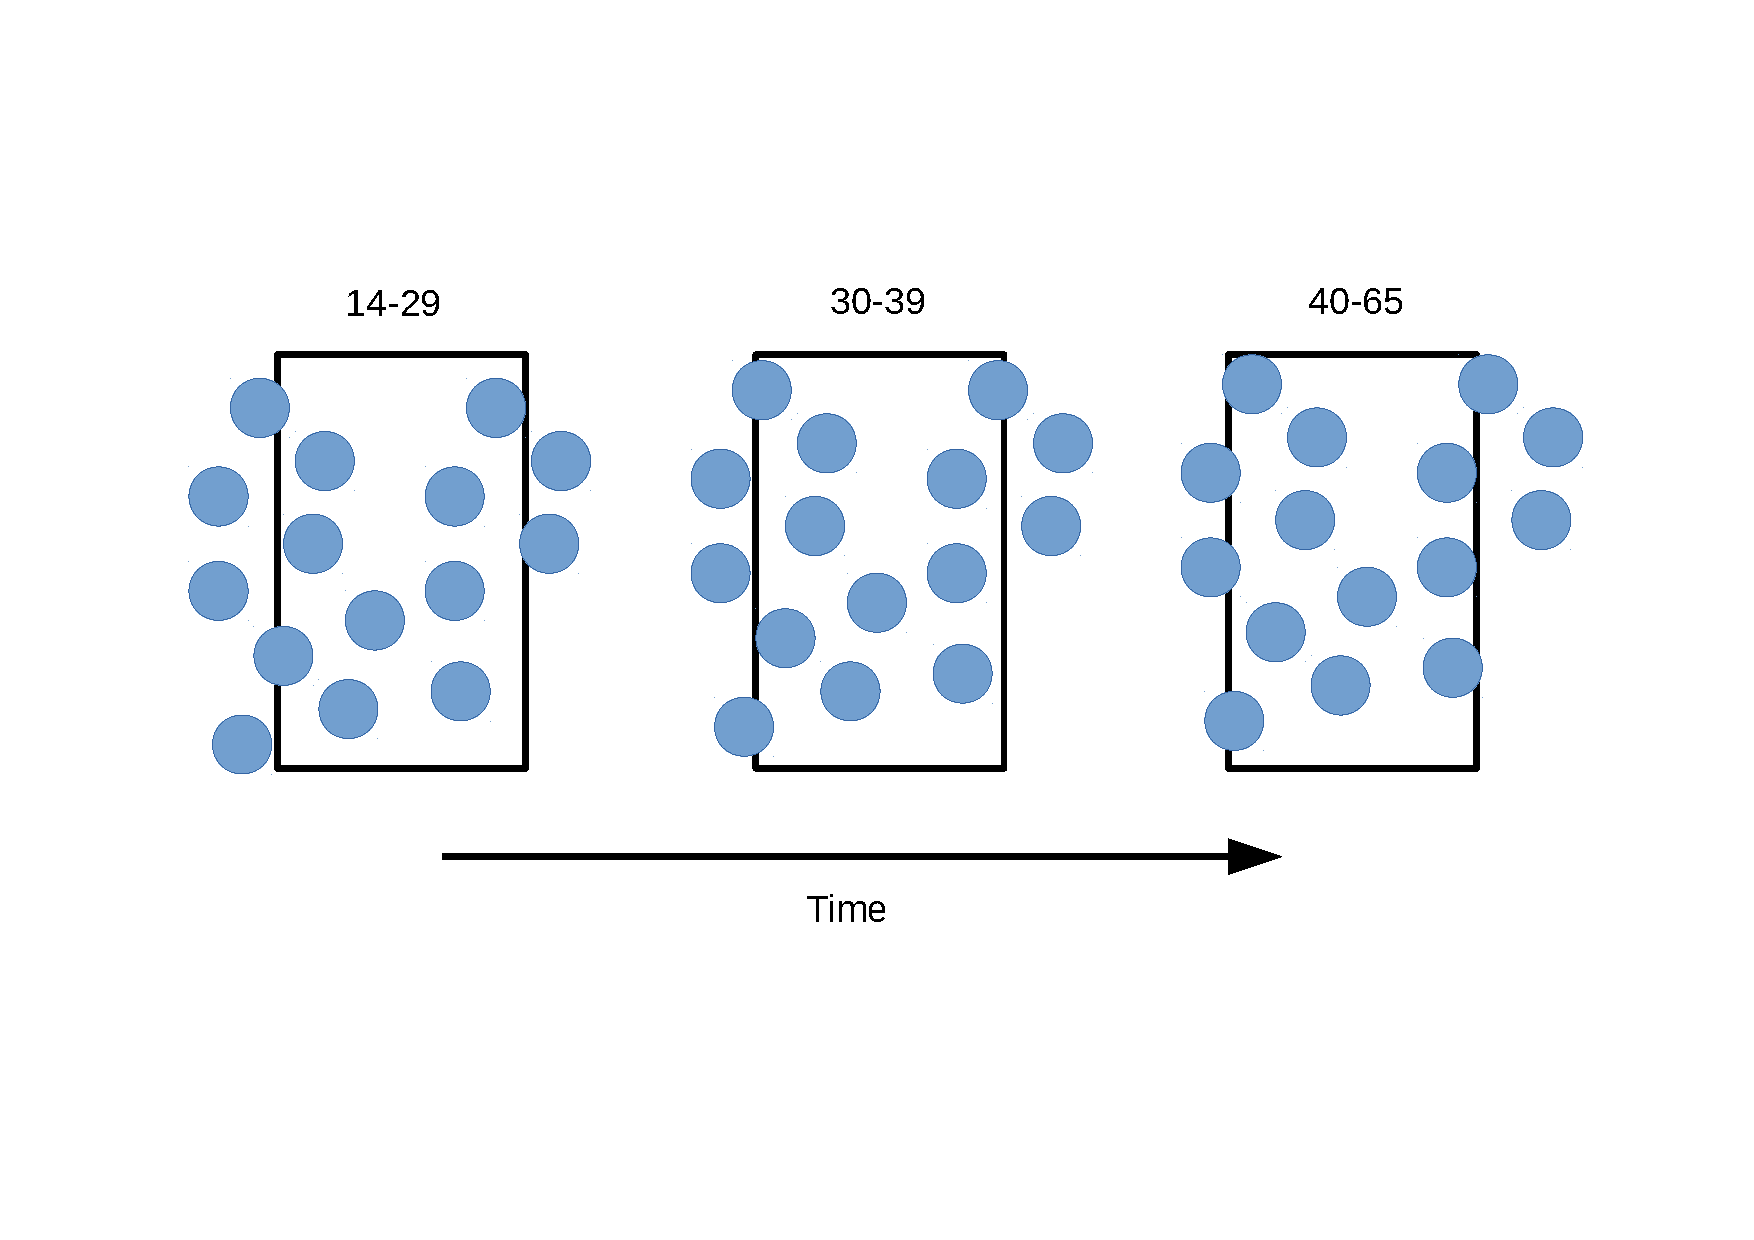
\includegraphics[width=0.7\linewidth]{IMGs/2.-New_features/Dinam_1.pdf}
	\caption{Static LSP network. The ages remain constant over the time. The time only affects the HPV contagion/clearing dynamics.}
	\label{fig:dinam1}
\end{figure}

Then, we evolve the ages of the nodes over the time. As long as the nodes do not change the age group, there is nothing to do. However, how do we \textit{recycle} the nodes that turn 64? And how do we transform the nodes in the first age group $14-29$ when they turn 30?  

To answer the first question, we propose to

\begin{itemize}
	\item preserve its sex in order to maintain the proportion males/females, 
	\item assign $14$ years old to the node, erase all its LSPs and transform it in susceptible,
	\item assign new LSPs according to the LSPs of the age group $14-29$ following the assortativity property.
\end{itemize}

To answer the second question, we propose to

\begin{itemize}
	\item preserve its sex and the infectious state, 
	\item erase all its LSPs and assign new LSPs according to the LSPs of the age group $30-39$ following the assortativity property.
\end{itemize}

This way, as time goes on, we will have the LSP structure by ages as we can see in the Figure \ref{fig:dinam2}.

\begin{figure}[h!]
	\centering
	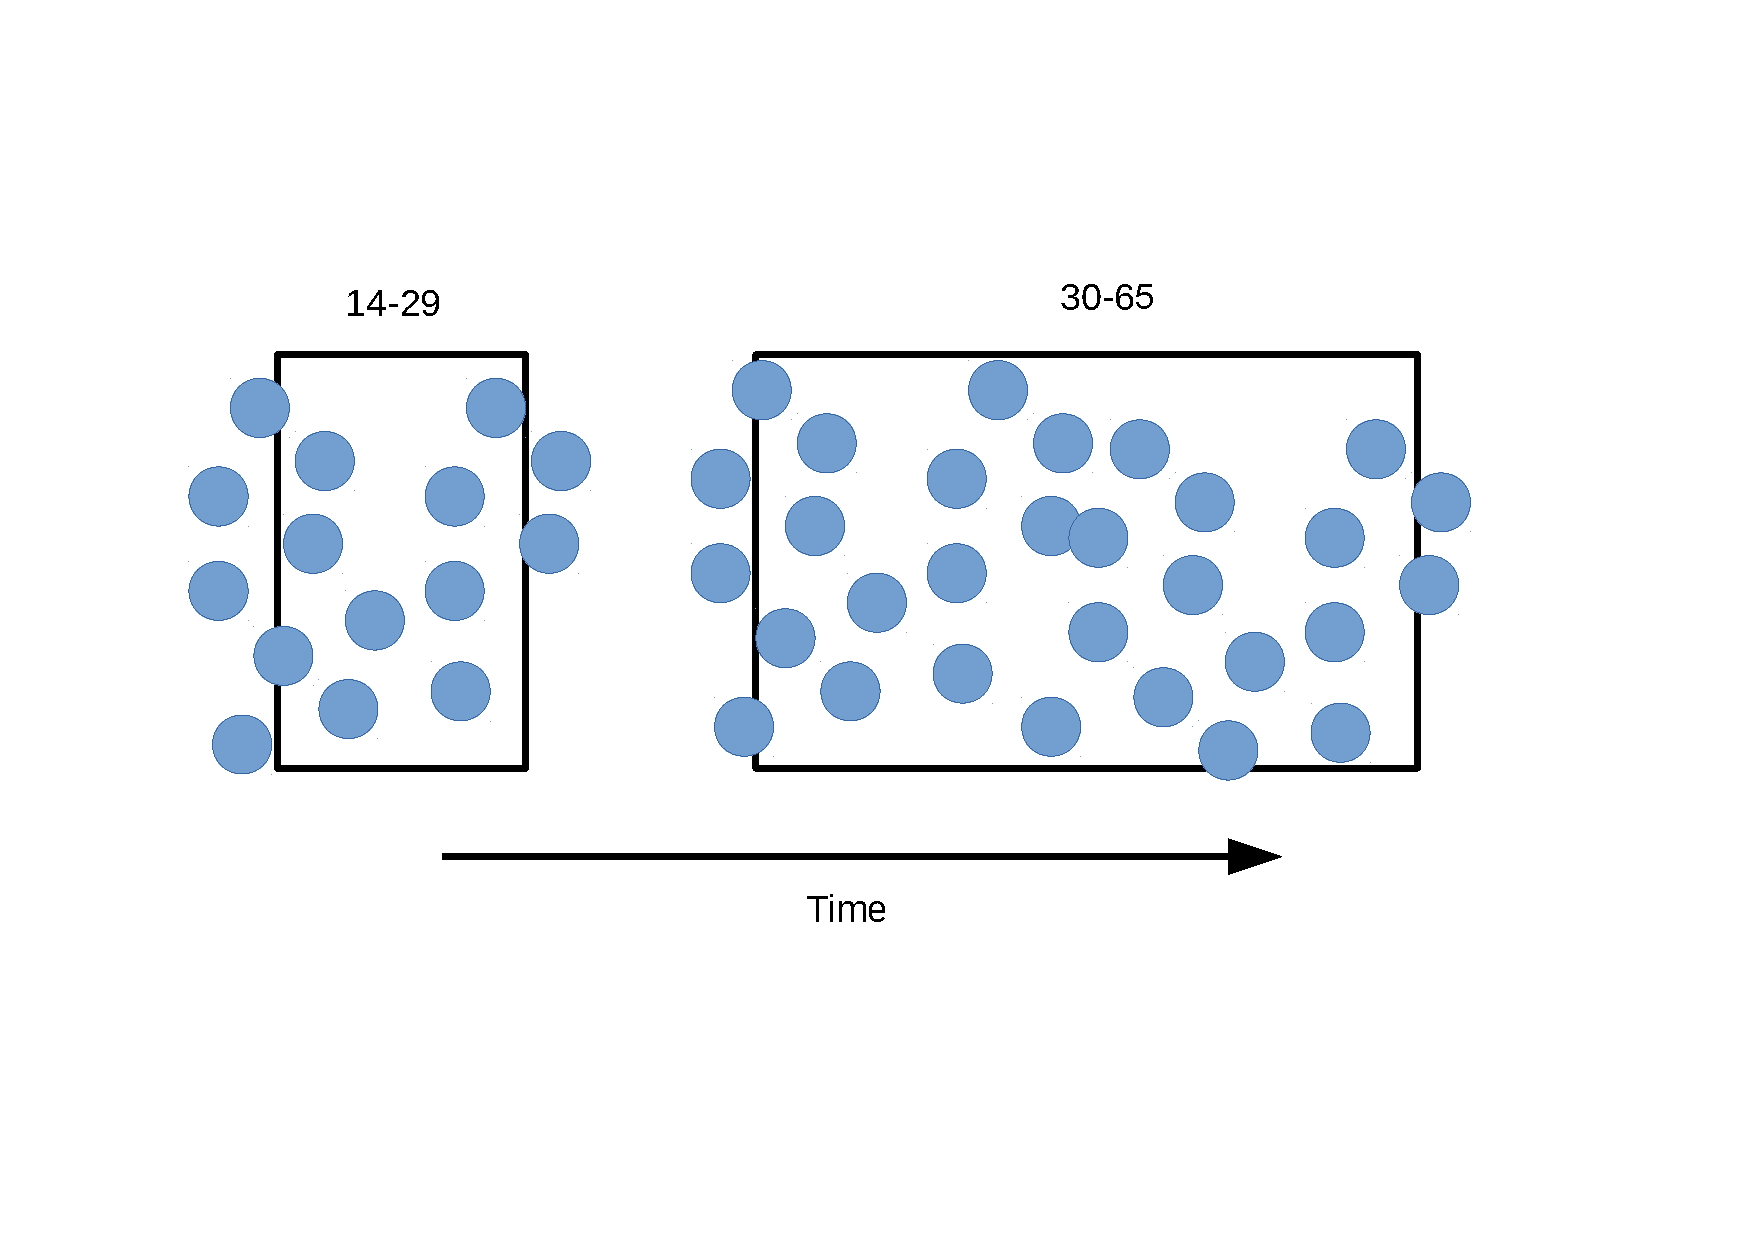
\includegraphics[width=0.7\linewidth]{IMGs/2.-New_features/Dinam_2.pdf}
	\caption{Dynamic LSP network. The ages evolve over the time. The age group 40-65 and their sexual behavior disappear when people grow.}
	\label{fig:dinam2}
\end{figure}

If the node is MSM (male who have sex with males), we perform the above procedure taking into account the division of age groups given in \cite{Durex2002}, $14-19$, $20-24$, $25-29$, $30-39$, $40-49$, $50-59$ and $60-64+$.

Taking into account that the global number of LSP in the age groups $40-64$ is less that in the age group $30-39$, as the time goes on, the global number of LSP in the whole network will increase and the transmission of HPV will also increase. However, the proposed approach may be considered as very conservative because the sexual behavior change in the last $10-15$ years seems to result in an increase of the sexual intercourses greater than the number that we can approach with the proposed dynamic network. Nevertheless, the lack of data do not allow us to quantify the mentioned change.

%, but we take advantage of the static model building and the calibrated model parameters. Furthermore, as we mentioned before, we do not have recent data about sexual behavior in Spain.

\section{When should we start the vaccination campaign?} 
When a realization executes, we use $500$ months to stabilize the static network, then, we change to a dynamic network. Thus, a key point arises and it is to decide in which time instant starts the vaccination schedule. We have performed a simulation with the selected $30$ sets of parameters with $2300$ months (around $191.6$ years) where the network turns dynamic from the month $500$. In the Figure \ref{fig:Estudio_ciclos} we can see the levels of prevalence predicted by the model for 18-64 years old men and women for HR and LR, over the next years.

\begin{figure}[h!]
	\centering
	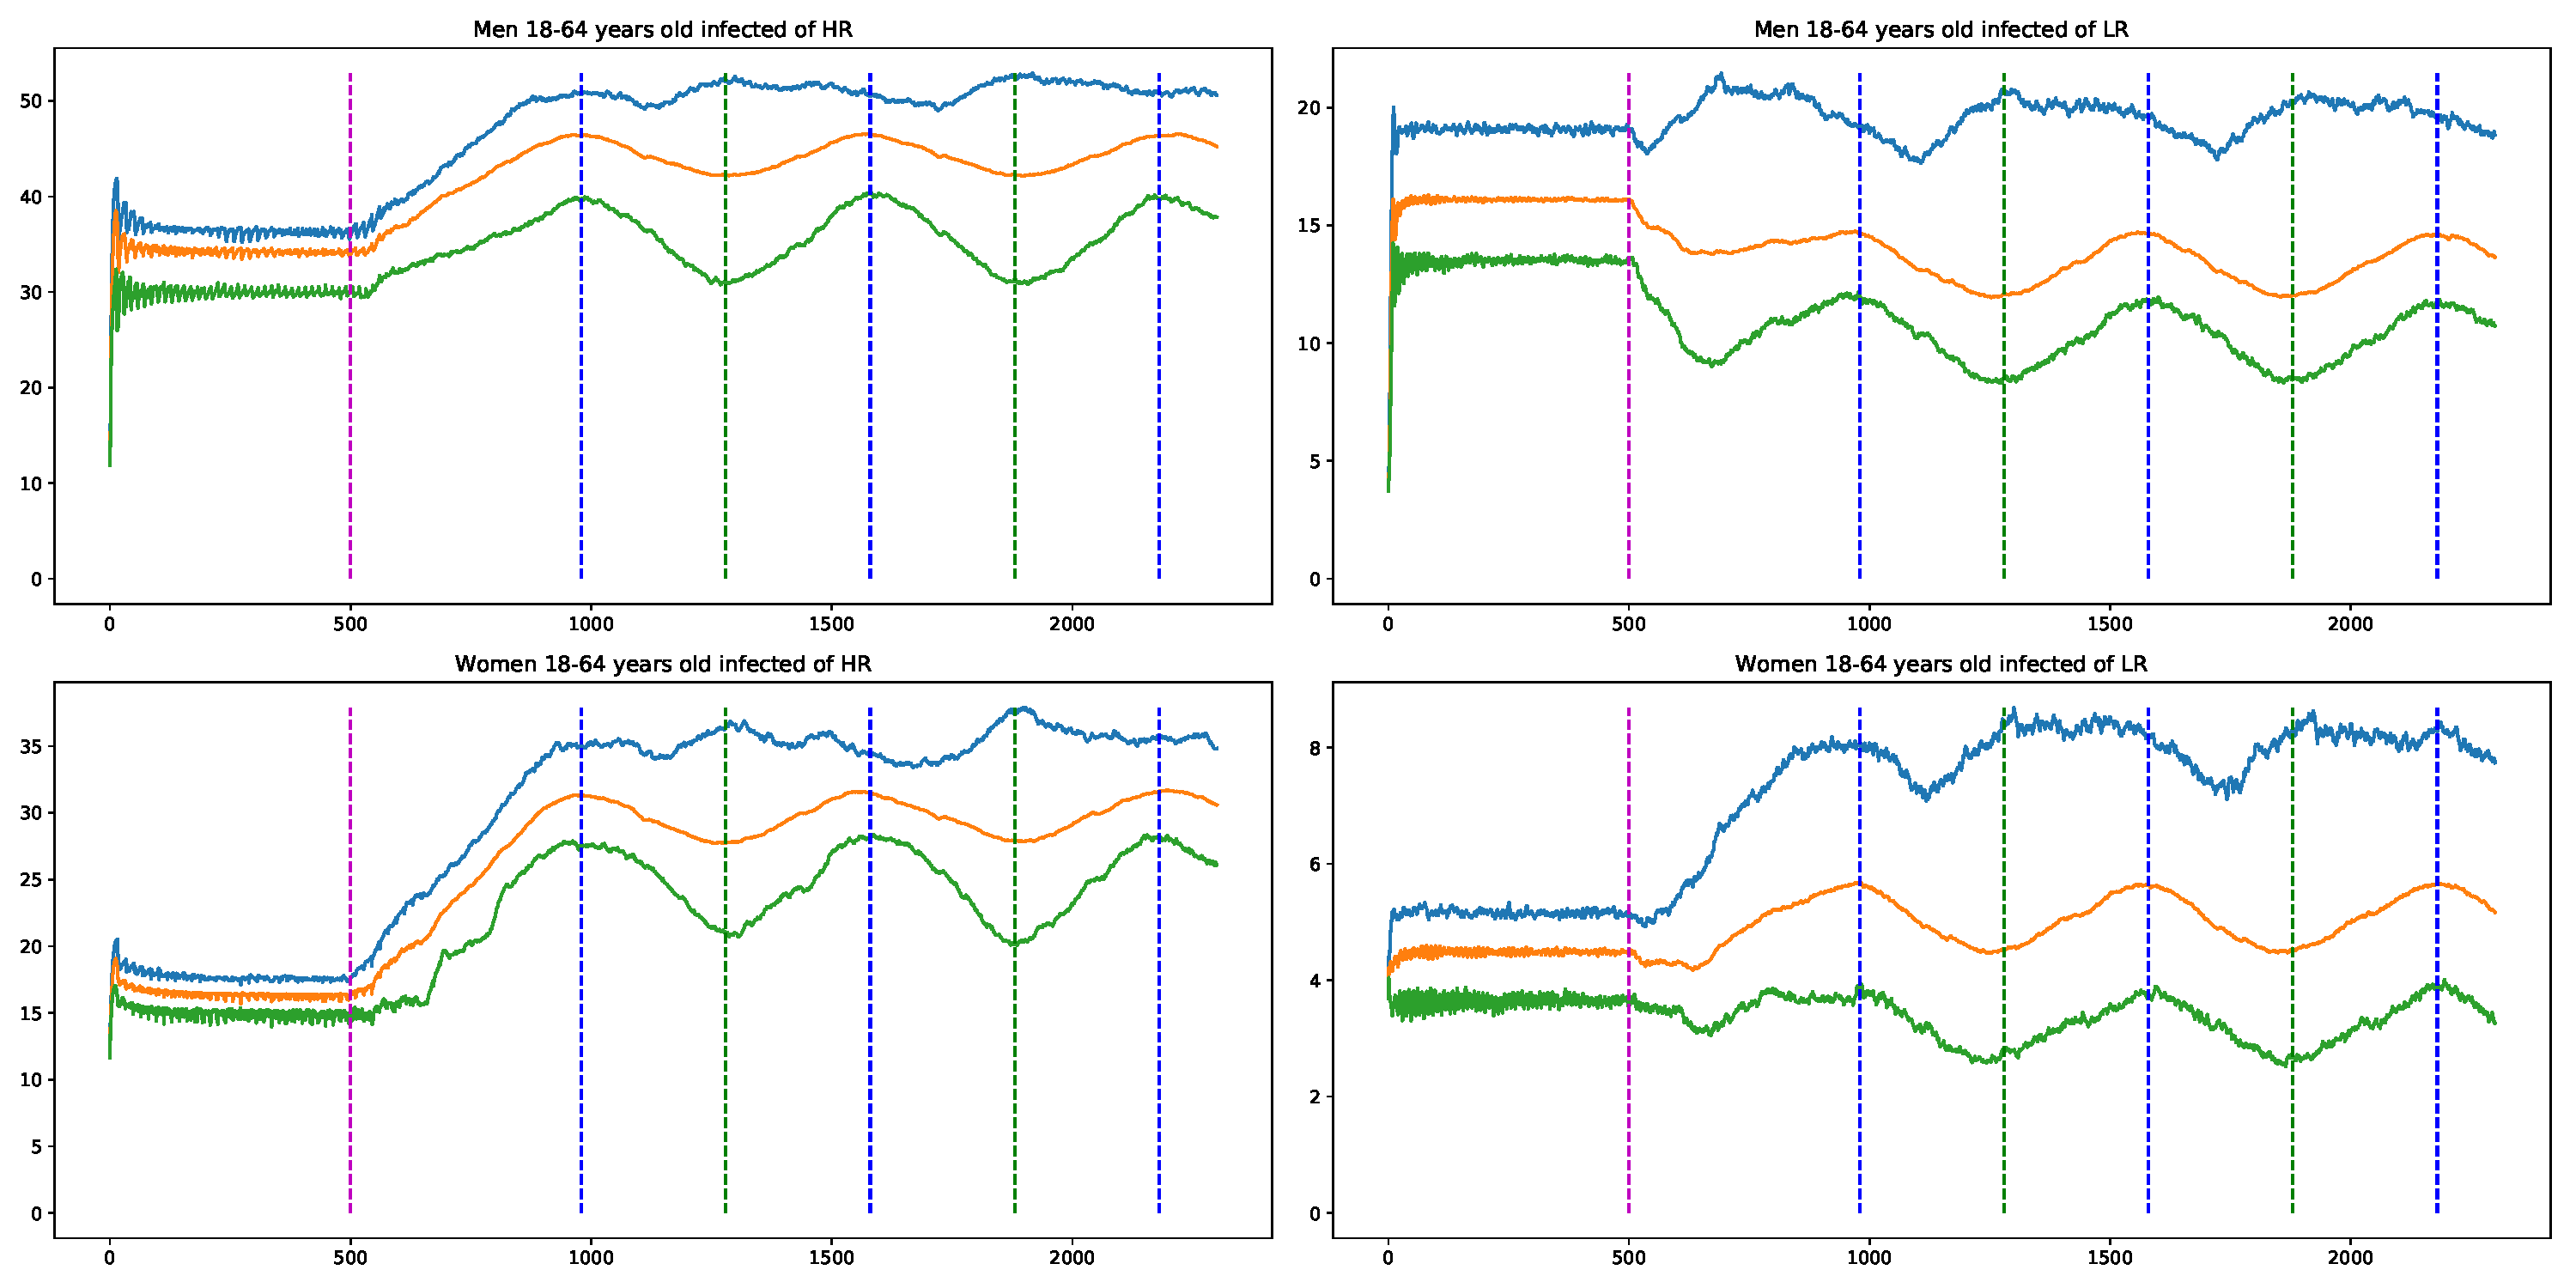
\includegraphics[width=\linewidth]{IMGs/2.-New_features/Estudio_ciclos.pdf}
	\caption{Mean and $95\%$ confidence intervals of the prevalence for 18-64 men and women for HR and LR. Vertical dashed lines indicate milestones of interest. Note the oscillations of the prevalence levels. The blue and green vertical lines correspond to the peaks and valleys of the oscillations. The magenta line, points the month 500 when dynamic network starts.}
	\label{fig:Estudio_ciclos}
\end{figure}

The Figure \ref{fig:Estudio_ciclos} shows the mean and $95\%$ confidence intervals of the $30$ simulations for the prevalence of men and women for HR and LR. The horizontal axis indicates the month and the vertical axis the percentage of infected. As it can be seen, there are oscillation in the evolution of the prevalence.

The vertical lines correspond to:
\begin{itemize}
	\item magenta: month $500$, the static network turns dynamic;
	\item blue: months $980$, $1580$ and $2180$, point out the peaks in the oscillations in the means and the percentiles. Between them, there are $600$ months ($50$ years), the time of a complete generation in the model;
	\item green: months $1280$  and $1880$, point out the valleys. Between the valleys there are also $50$ years, and $25$ years between a peak and a valley. 	
\end{itemize}

In some test executions with vaccination, we have observed that, if we start the vaccination schedule when the prevalence is in the decreasing part (towards a valley) of the oscillation, the herd immunity appears very much sooner than when we start the vaccination schedule in the increasing part (towards a peak).

If we take into account that in the paper \cite{ali2013genital}, the authors reports extraordinary results in Australia, where two years after the vaccine was introduced, the proportion of genital warts diagnosed declined by a $59\%$ in vaccine eligible young women aged 12--26 years in $2007$, and by $39\%$ in men of the same age, we conjecture that, if there are oscillations in the prevalence of HPV over the time, they have taken advantage of a decreasing part of an oscillation.

Recall that our goal is to determine the appropriate month where the vaccination schedule starts, trying to save computations and favoring the apparition of the herd immunity effect as soon as possible, in order to minimize the opposite effect when the oscillation is in the increasing trend if we have vaccinated a large enough number of individuals.

The oscillations in all the cases, men, women, HR and LR, are very similar, as we can see in the Figure \ref{fig:Estudio_ciclos}, except, maybe in some upper percentiles. Also, there are similarities from the first peak, in valleys and peaks. Therefore, in order to take the maximum advantage of the decreasing trends and to save computation, we are going to select the earliest peak, the month $980$, as the starting point for the vaccination.

\section{Introducing vaccination} 
For our simulations, we are going to consider the vaccine GARDASIL9 \cite{gardasil9}. GARDASIL9 is a vaccine indicated in girls and women 9 through 45 years of age for the prevention of  cervical, vulvar, vaginal, and anal cancer caused by HPV types 16, 18, 31, 33, 45, 52, and 58,  genital warts caused by HPV types 6 and 11, and precancerous or dysplastic lesions caused by above HPV types. It is also indicated in boys and men 9 through 45 years of age for the prevention of anal cancer caused by HPV types 16, 18, 31, 33, 45, 52, and 58, genital warts caused by HPV types 6 and 11, and precancerous or dysplastic lesions caused by above HPV types.

The HPV types 6/11 are LR and the remainder (16, 18, 31, 33, 45, 52, and 58) are HR. Thus, GARDASIL9 prevents against $90\%$ of genital wart cases and $90\%$ of the cancer cases \cite{Hartwig2015}. Although GARDASIL9 may prevent partially against other HPV types, for modeling purposes we assume that it does not happen. Therefore, it would be interesting to introduce changes in order to monitor if a node is infected by HPV types included in GARDASIL9 or not, and then, to simulate accurately the prevention effect of the vaccine.

Following the study conducted in \cite{castellsague2012prevalence}, if a woman is infected by HPV LR, the probability to be only infected by 6/11 is $34.23\%$, $63.06\%$ only infected by others than 6/11 and $2.70\%$ to be infected by both. Also, if a woman is infected by HPV HR, the probability to be infected only by 16/18/31/33/45/52/58 is $30.44\%$, $23.66\%$ only infected by others than 16/18/31/33/45/52/58 and $45.90\%$ by both. Due to the lack of information about men, we will also use the above percentages for men.

Then, before starting the vaccination, we label men and women as infected of HPV LR 6/11 or infected of HPV LR other than 6/11 or infected of both, following the above percentages. Analogously, we label men and women as infected of HPV HR 16/18/31/33/45/52/58 or infected of HPV HR other than 16/18/31/33/45/52/58 or infected of both.

Once these assignments are done, we continue with the HPV transmission dynamics including the vaccination, taking into account the new labels we included. If a node has been vaccinated, it can be infected by the types of HPV different to those that GARSDASIL9 prevents and, in this case, they will never be infected of 6/11 nor 16/18/31/33/45/52/58. If a node has not been vaccinated, can be infected by any HPV type. 

The assumed effectiveness of the vaccine is $96.5\%$.

\section{Introducing vaccination loss protection}
In the previous section we assume that the protection of GARDASIL9 is forever. In fact, until now, people vaccinated by GARDASIL (previous version of GARDASIL9) do not have experienced any loss in the protection. But this does not mean that it could happen in the future. 

In fact, we want to simulate the worst possible scenario, that is, the sudden drop to zero of the protection. To simulate this possibility, we will introduce a new parameter that represents the time after the vaccination where the protection is complete. Therefore, after this time, the vaccinated individual will behave as a non-vaccinated individual.

\section{Introducing variations in the vaccination coverage}
One of our goals is to simulate scenarios where variations in the vaccination coverage have been occurred and we want to study the effect in the global protection against HPV due to these variation of the coverage. To simulate these scenarios, we will include into the model vectors of coverage, indicating the vaccine coverage every month, and vaccinating the people following these variable coverages. 

%Cap�tulo 5
% !TeX spellcheck = en_US
%Aqui hay que mezclar sabiamente y en orden el paper de Viruses y los resultados del informe
\chapter{Model validation: The Australian case}\label{Australiano}

In this chapter we are going to check if we can obtain similar results to those in \cite{ali2013genital,fairley2009rapid} using the calibration parameters.

As we introduced in Chapter \ref{intro} \cite{ali2013genital} there is a decrease on the number of infected persons and the number of persons with GW is already reported for Australia after two years of administering vaccinations to young girls. These results were more impressive than predicted by continuous models.

To check the reliability of the model, we simulated the HPV vaccination campaign carried out in Australia \cite{ali2013genital}, and compared them with the actual impact published \cite{ali2013genital}. In 2007, Australian health authorities started a vaccination program for 12--13 year-old girls with a~coverage of $73\%$ ($83\%$ in the first dose, $80\%$ in the second dose and $73\%$ in the third dose). In addition, from 2007 to 2009, there was a catch-up vaccination program for women aged 13--26 with a decreasing coverage with age until $52\%$ in women aged 20--26. The results can be summarized as follows \cite{ali2013genital}:

\begin{itemize}
	\item Two years after the vaccine was introduced, the proportion of genital warts diagnosed declined by a $59\%$ in vaccine eligible young women aged 12--26 years in $2007$, and by $39\%$ in men of the same age.
	\item No significant decline was observed in women or men older than $26$ years old, non-resident young women, or men who have sex with men (MSM).
\end{itemize}

Two different scenarios were considered to be simulated:

\begin{itemize}
	\item Scenario 1: vaccination of $83\%$ of the $14$ year-old girls (or younger girls) plus a catch-up with coverage $73\%$ for 14--26 year-old women.
	\item Scenario 2: vaccination of $73\%$ of $14$ year-old girls (or younger girls) plus a catch-up with a~vaccination coverage of $52\%$ for 14--26 year-old women.
\end{itemize}

These simulations represented the upper and lower bounds of the scenario implemented in Australia. 

\section{How to measure the decline}\label{sec:decline}%esto lo borré de otro capítulo y lo pongo ya aqui

We call $I$ the number of infected women of LR HPV 6 and/or 11 just before the starting of the vaccination campaign; we call $V = ( v_1, \ldots, v_N)$ to the number of infected women of LR HPV 6 and/or 11 every month from the starting of the vaccination program until the end of the simulation. Then,~the~vector 

\begin{equation}
100 \times \left( 1-\displaystyle\frac{v_1}{I}, \ldots, 1-\displaystyle\frac{v_N}{I} \right) \; 
\end{equation}

is a measure of the percentage of decline of the number of infected women of LR HPV 6 and/or 11 after the beginning of the vaccination campaign. This will also be applied to men and MSM.

In order to compare GW data given in \cite{ali2013genital} with our model, results referred to infected women of LR HPV 6 and/or 11, we should take into account that, whether a fixed proportion of HPV 6 and/or 11 infected individuals develops warts, the percentage of decline in warts and in infected women of LR HPV 6 and/or 11 will be comparable. 

Another important issue for the natural history of the disease is the persistence of the infection \cite{campos2014updated}. Our model does not consider the persistence ``a priori'', but we derive the cases of genital warts from the number of cases of infected individuals by taking this data into account.

\section{Does our model return similar values to those in \cite{ali2013genital}?}

In this section, we are going to show figures about prevalence and decline of the percentage of women, men and MSM infected of LR 6/11, the HPV type responsible of $90\%$ of genital warts. Taking into account that genital warts, in average, use to appear 6 months after the infection, the figures about prevalence or decline will be a good estimation of the prevalence and the  decline of genital warts.  

Figure \ref{fig:prev_AUS_6_11} shows the percentage of women, men and MSM aged 14-26 infected of LR 6/11 after starting the vaccination program in both simulated scenarios. We can see the fast decrease for women and men in both scenarios from the very beginning. MSM remain constant. 

\begin{figure}[!]
	\centering
	\begin{tabular}{cc}
		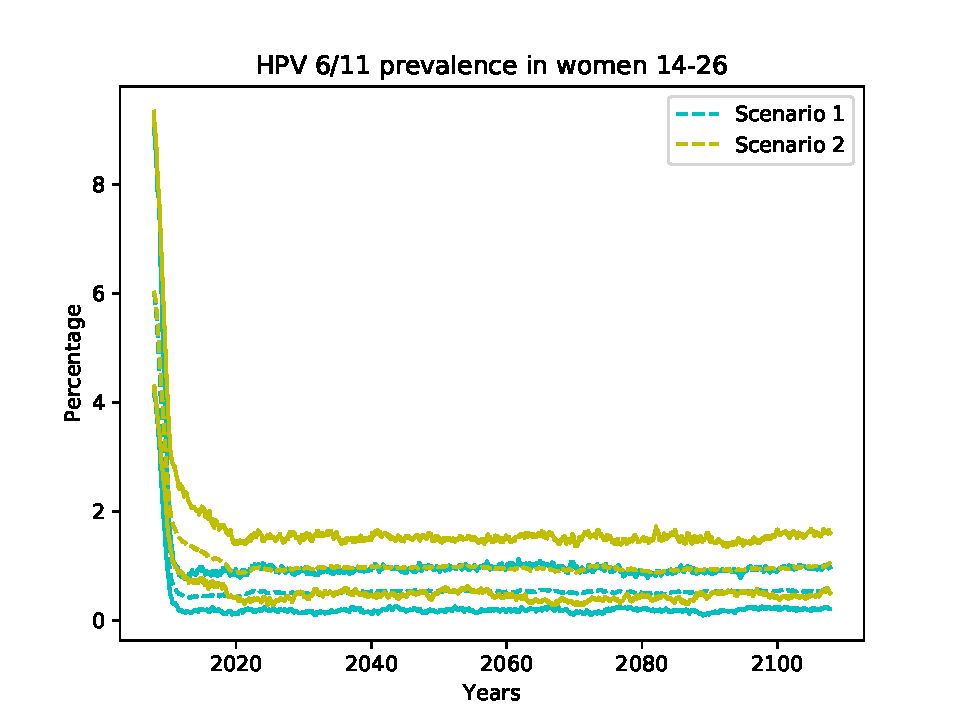
\includegraphics[width=0.5\linewidth]{IMGs/3.-Australia/retrieve_14_26_verr_muj.pdf}	& 
		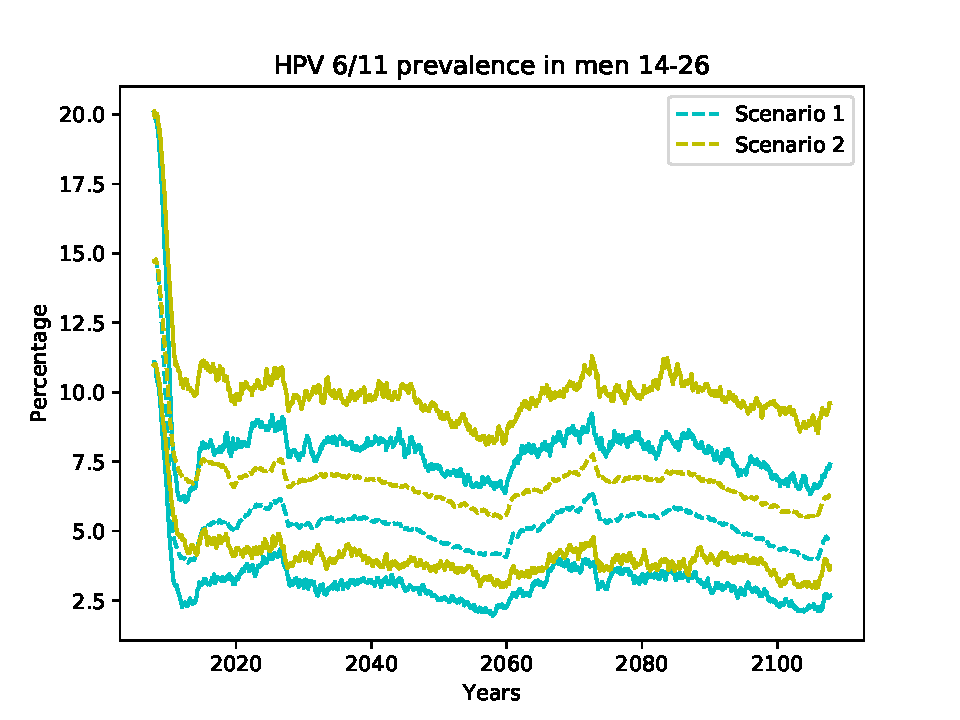
\includegraphics[width=0.5\linewidth]{IMGs/3.-Australia/retrieve_14_26_verr_hom.pdf}  \\ 
		(a)	& (b) \\ 
		\multicolumn{2}{c}{ 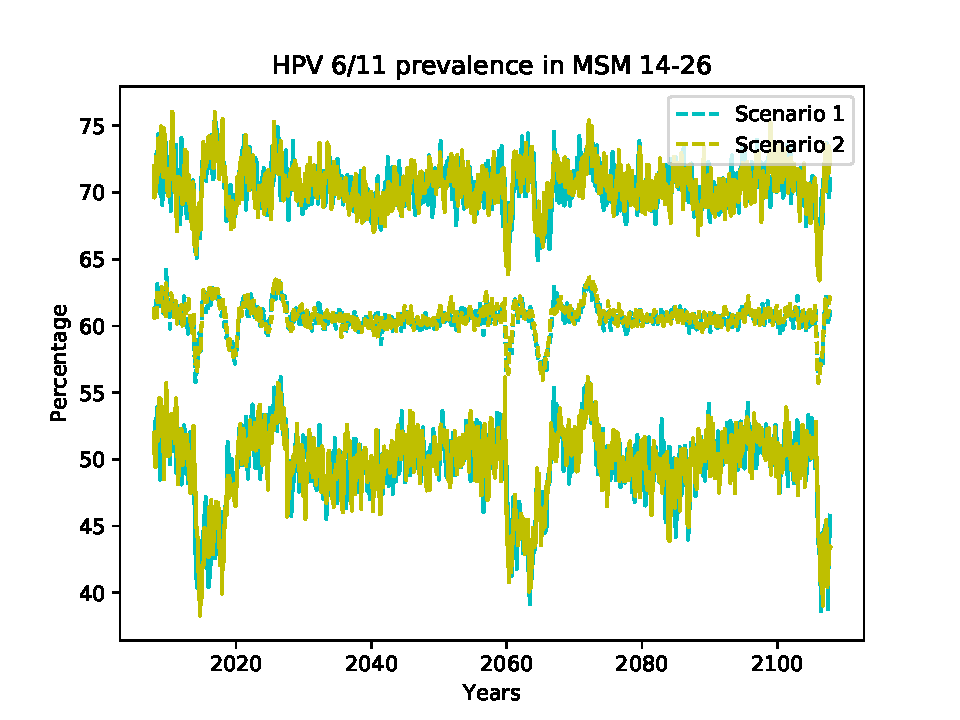
\includegraphics[width=0.5\linewidth]{IMGs/3.-Australia/retrieve_14_26_verr_MSM.pdf} } \\ 
		\multicolumn{2}{c}{(c)} \\ 
	\end{tabular} 
	\caption{Percentage of women (a), men (b) and MSM (c) aged 14-26 infected of LR HPV 6 and/or 11 after the implementation of the vaccination program. The cyan lines correspond to the average and $95\%$ confidence interval for Scenario 1 and the yellow lines to Scenario 2.  We can see the fast decrease for women and men in both scenarios from the very beginning. However, there is not effect on MSM.}
	\label{fig:prev_AUS_6_11}	
\end{figure}

In Figure \ref{fig:decline_AUS_6_11}, we have plotted the same data as in Figure \ref{fig:prev_AUS_6_11} but from another point of view: the average percentage of decline of women and men infected of LR HPV 6 and/or 11. As the vaccination program progresses over time, the percentage of decline obviously grows. After 2 years, the model shows a decline of

\begin{itemize}
	\item Scenario 1: $72.0\%$ with CI $95\%$ $[67.7\%, 76.5\%]$ for women and $38.9\%$ with CI $95\%$ $[32.0\%, 45.5\%]$ for men. 
	\item Scenario 2: $54.8\%$ with CI $95\%$ $[48.5\%, 59.0\%]$ for women and $27.7\%$ with CI $95\%$ $[21.3\%, 34.5\%]$ for men. 
\end{itemize}

Australian reported levels of decline ($59\%$ in women and $39\%$ in men aged 14-26) will be reached by the model after

\begin{itemize}
	\item Scenario 1: $1.66$ years with CI $95\%$ $[1.5, 1.75]$ for women and $2.0$ years with CI $95\%$ $[1.75, 2.16]$ for men,
	\item Scenario 2: $2.1$ years with CI $95\%$ $[2.0, 2.33]$ for women and $2.42$ years with CI $95\%$ $[2.08, 2.83]$ for men.
\end{itemize}

\begin{figure}[!]
	\centering
	\begin{tabular}{cc}
		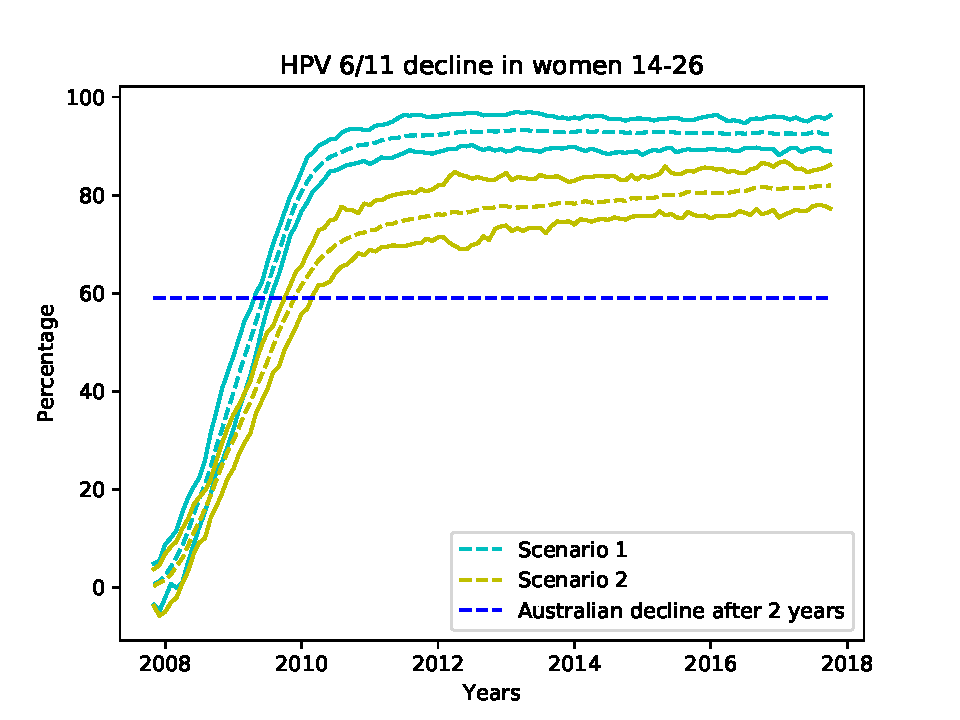
\includegraphics[width=0.45\linewidth]{IMGs/3.-Australia/decline_14_26_verr_muj.pdf}	& 
		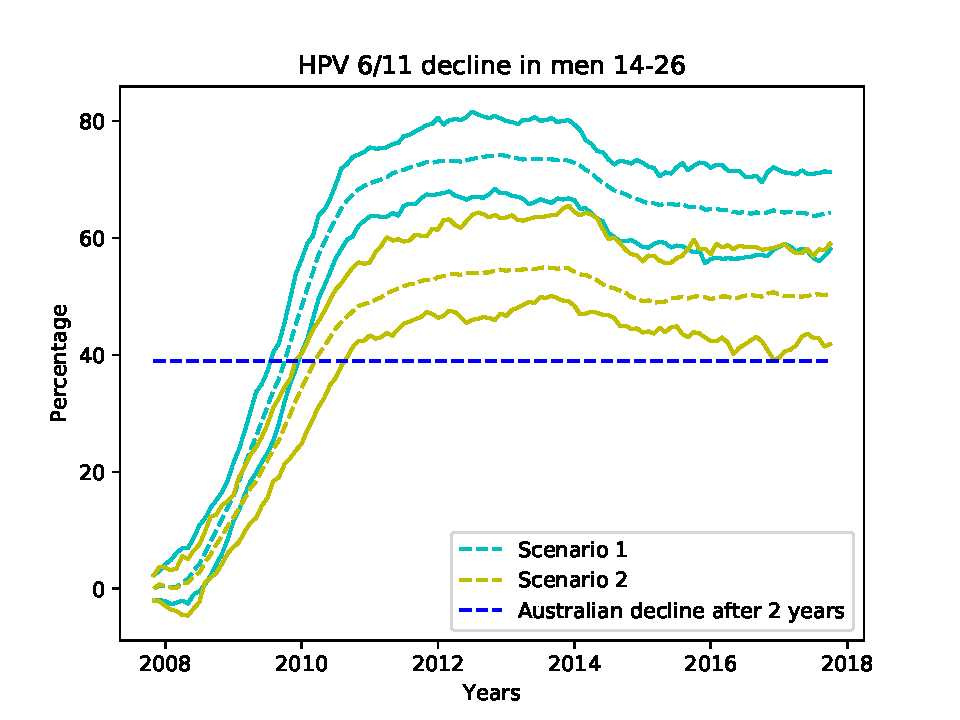
\includegraphics[width=0.45\linewidth]{IMGs/3.-Australia/decline_14_26_verr_hom.pdf}  \\ 
		(a)	& (b) 
	\end{tabular} 
	\caption{Percentage of decline of women (a) and men (b) aged 14-26 infected of LR HPV 6 and/or 11 (and consequently of genital warts) after the implementation of the vaccination program. The cyan lines correspond to the average and $95\%$ confidence interval for Scenario 1 and the yellow lines to Scenario 2. After 2 years, the model shows a decline of $72\%$ for Scenario 1 and $54.8\%$ for Scenario 2, in average, for women and $38.9\%$ for Scenario 1 and $27.7\%$ for Scenario 2, in average, for men.}
	\label{fig:decline_AUS_6_11}
\end{figure}

No significant impact on the rate of infection was observed in men aged 27-64, 2 years after the implementation of the vaccination program (Figure \ref{fig:decline_AUS_6_11_27_64}) and the same in women and MSM agreeing the observations reported in \cite{ali2013genital}. It can be explained by the fact that, usually, individuals have sexual intercourses with people more or less the same age. 

Then, our model predicts figures close to the ones given in \cite{ali2013genital}.

\begin{figure}[!]
	\centering
	\begin{tabular}{cc}
		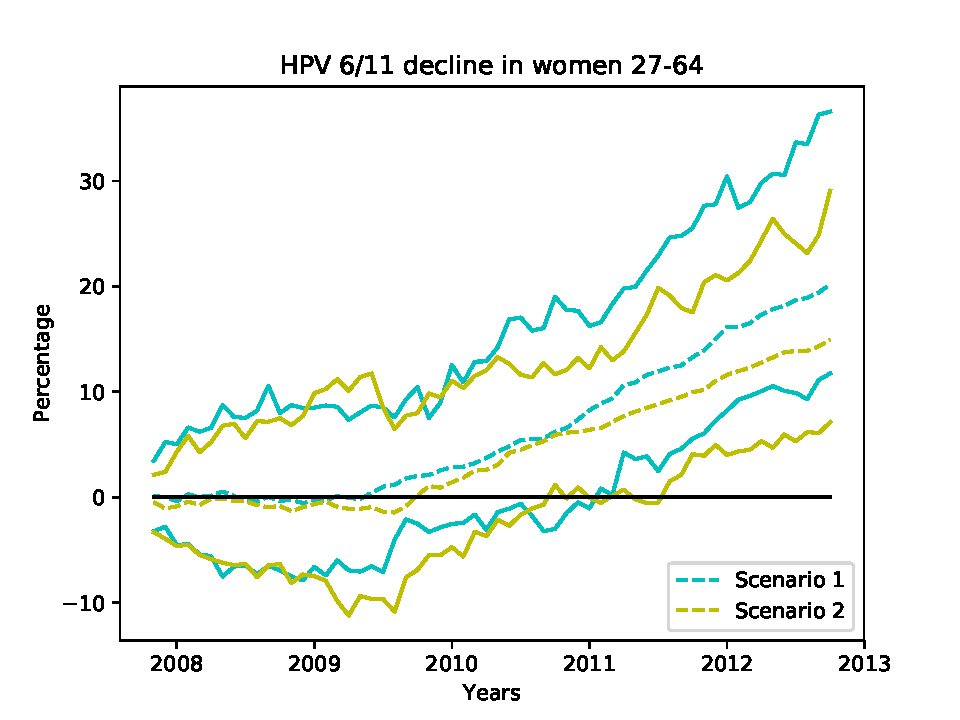
\includegraphics[width=0.5\linewidth]{IMGs/3.-Australia/decline_27_64_verr_muj.pdf}	& 
		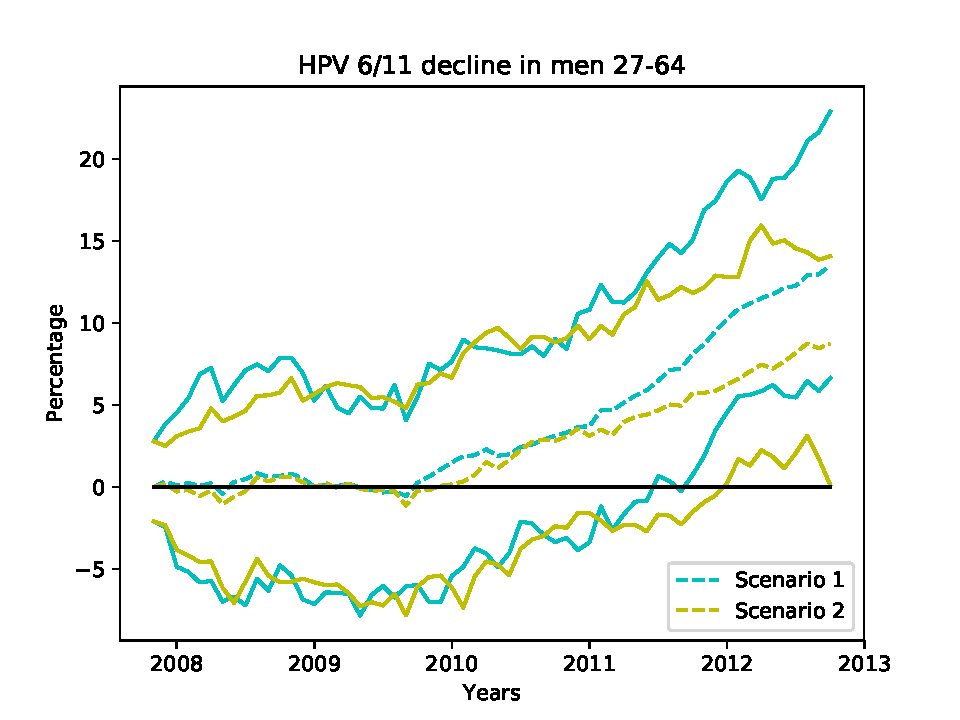
\includegraphics[width=0.5\linewidth]{IMGs/3.-Australia/decline_27_64_verr_hom.pdf}  \\ 
		(a)	& (b) \\ 
		\multicolumn{2}{c}{ 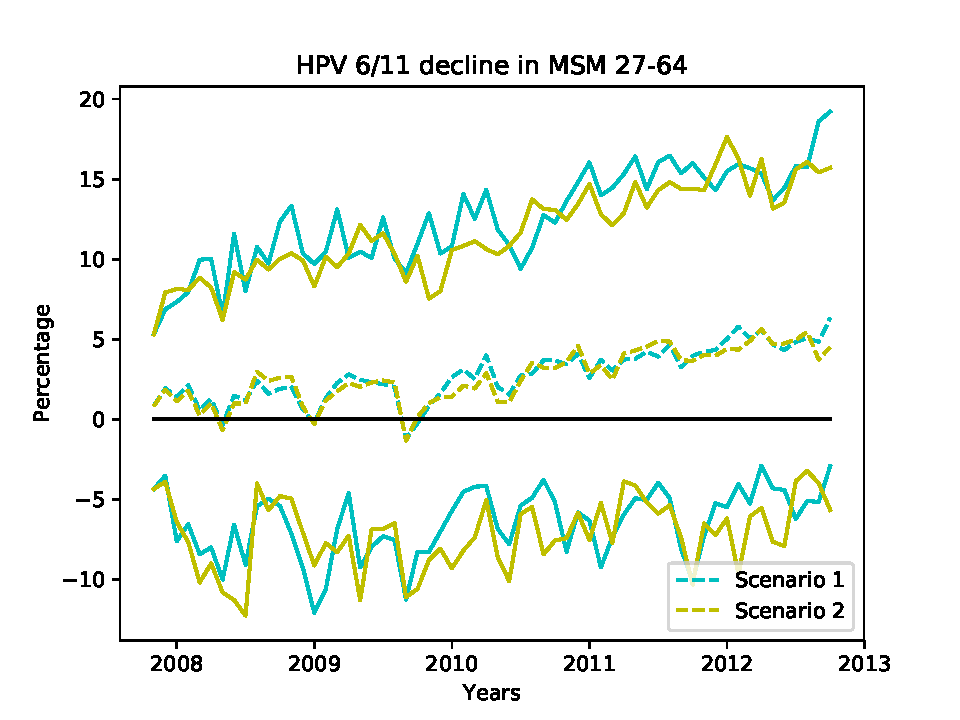
\includegraphics[width=0.5\linewidth]{IMGs/3.-Australia/decline_27_64_verr_MSM.pdf} } \\ 
		\multicolumn{2}{c}{(c)} \\ 
	\end{tabular} 
	\caption{Percentage of decline of women (a), men (b) and (c) MSM aged 27-64 infected of LR HPV 6 and/or 11 (and consequently of genital warts) after the implementation of the vaccination program in both scenarios. The cyan lines correspond to the average and $95\%$ confidence interval for Scenario 1 and the yellow lines to Scenario 2. Notice that, in average, no significant decline appears in the 5 years after the implementation of the vaccination program.}
\label{fig:decline_AUS_6_11_27_64}
\end{figure}

\section{Study of the herd immunity effect over HPV LR infection}
The herd immunity effect in both scenarios is shown in Figure \ref{fig:decline_AUS_6_11_14_64} for women, men and MSM. Notice that, in men and MSM, any decline is due to herd immunity. The decline in the whole female population appears when the lines representing their decline are over the vaccination lines (blue for Scenario 1 and green for Scenario 2) also shown in this figure. The herd immunity effect starts after 

\begin{itemize}
	\item for women
	\begin{itemize}
		\item Scenario 1: $0.58$ years with CI95\% $[0.0, 22.1]$.
		\item Scenario 2: $0.58$ years with CI95\% $[0.0, 22.1]$.
	\end{itemize}
	\item for men
	\begin{itemize}
		\item Scenario 1: $0.0$ years with CI95\% $[0.0,0.83]$.
		\item Scenario 2: $0.0$ years with CI95\% $[0.0,0.83]$.	
	\end{itemize}
\end{itemize}

The herd immunity effect starts very quickly for men. For MSM, there is not a clear herd immunity effect because the decline is stable over the time. For women, we can see that, practically, the CI$95\%$ decline lines are over the vaccination lines in both scenarios. This means that, in the worst case, only the vaccinated women will be protected and in the best case, almost all women will be protected by vaccination or by herd immunity effect.

\begin{figure}[!]
	\centering
	\begin{tabular}{cc}
		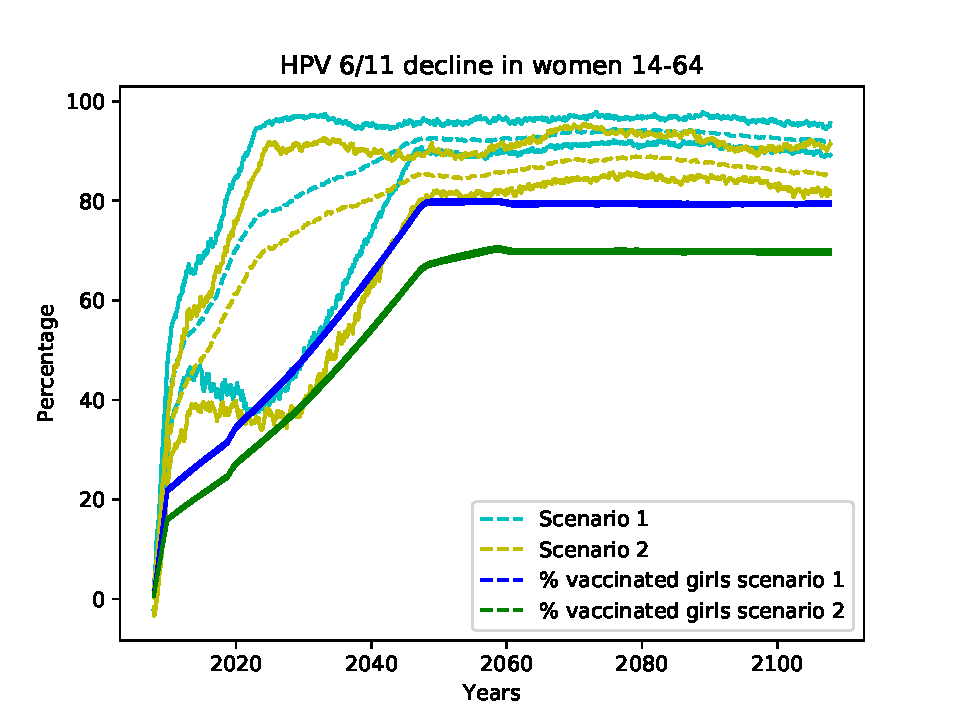
\includegraphics[width=0.45\linewidth]{IMGs/3.-Australia/decline_14_64_verr_muj.pdf}	& 
		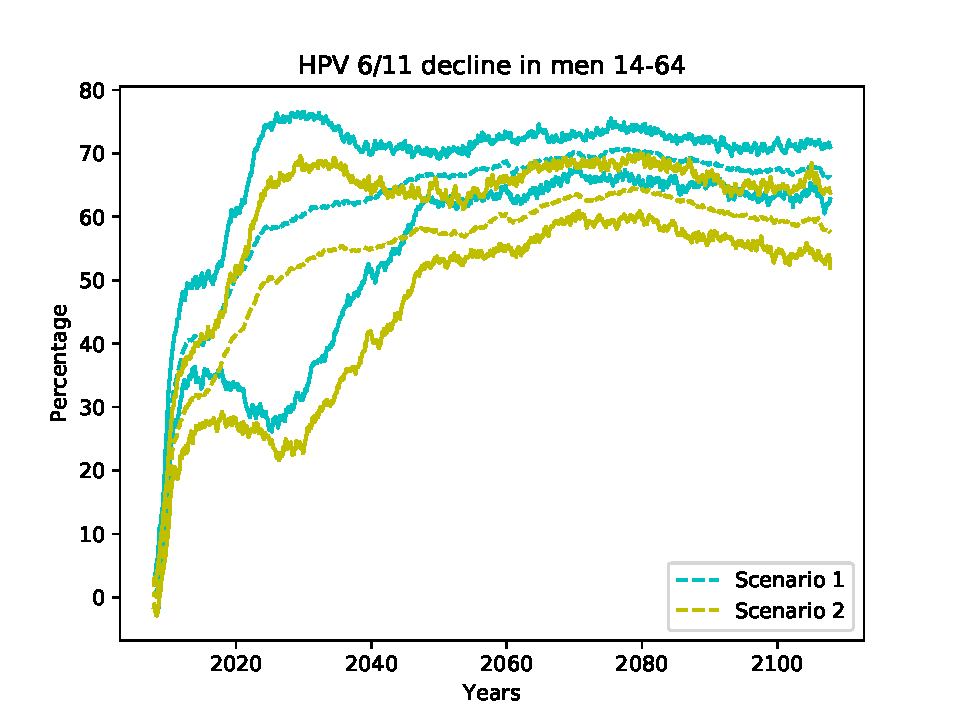
\includegraphics[width=0.45\linewidth]{IMGs/3.-Australia/decline_14_64_verr_hom.pdf}  \\ 
		(a)	& (b) \\ 
		\multicolumn{2}{c}{ 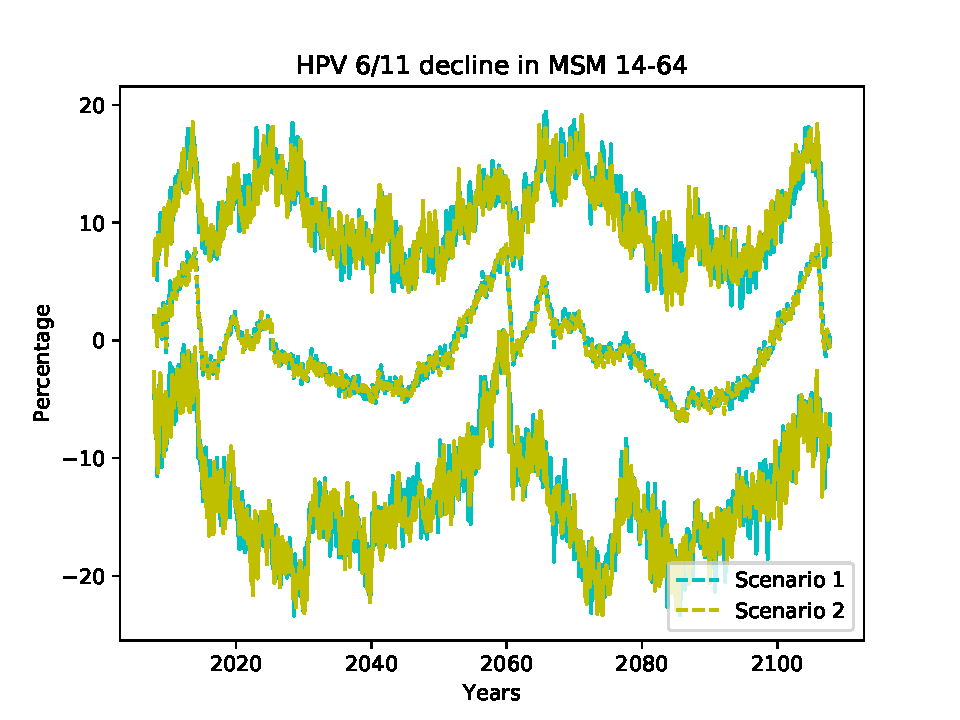
\includegraphics[width=0.5\linewidth]{IMGs/3.-Australia/decline_14_64_verr_MSM.pdf} } \\ 
		\multicolumn{2}{c}{(c)} \\ 
	\end{tabular} 
	\caption{Percentage of decline of women (a), men (b) and MSM (c) aged 14-64 for the vaccination program in Australia. The cyan lines correspond to the average and $95\%$ confidence interval for Scenario 1 and the yellow lines to Scenario 2. In the figure (a), blue and green lines correspond to women vaccination percentage for Scenario 1 and 2, respectively. Notice that the herd immunity effect contributes to the decline in the number of infections in men and the decline in the number of infections for unvaccinated women. This latter can be seen when the decline lines are over the vaccination line. However, any herd immunity effect can be seen in MSM.}
	\label{fig:decline_AUS_6_11_14_64}
\end{figure}

Notice that the herd immunity effect is very clear within the CI$95\%$ both for women and men, but it does not appear in the MSM population. In the best case scenario, the MSM subpopulation achieves a constant protection level of $10\%-15\%$. This could be attributed to the way in which the MSM individuals are connected: with a very large number of LSPs among them and some casual links with women with large LSPs.

\section{Effect of the reduction of the vaccine effectiveness in the catch-up vaccination}\label{sec:australia_sfuka}
In the reference \cite{Skufca}, the authors performs a literature review where they show that the effectiveness of the HPV vaccine on cervical abnormalities is between $20\%-54\%$ instead of the assumed $96.5\%$. This means that the vaccine effectiveness experiments a reduction in those women who had previous contact with the virus.

To study the effect of this catch-up loss of the effectiveness, we propose the simulation of the following two scenarios: 

\begin{itemize}
	\item Scenario 1: vaccination of $83\%$ of the $14$ year-old girls (or younger girls) plus a catch-up with coverage $73\%$ for 14--26 year-old women with $54\%$ of catch-up effectiveness.
	\item Scenario 2: vaccination of $73\%$ of $14$ year-old girls (or younger girls) plus a catch-up with a~vaccination coverage of $52\%$ for 14--26 year-old women with $20\%$ of catch-up effectiveness.
\end{itemize}

The above scenarios consists of a variation of the scenarios already proposed  for Australia at the beginning of this chapter, but now, considering the reduction of the effectiveness in the catch-up vaccination. The simulations consider upper and lower scenarios. 

In the following, we present the compared results with the scenarios without loss of effectiveness in the catch-up vaccination. Then, after 2 years, the model declines are

\begin{itemize}
	\item Ali et al. \cite{ali2013genital}: $59\%$ for women and $39\%$ for men.
	\item Catch-up without loss of effectiveness:
	\begin{itemize}
	\item Scenario 1: $72.0\%$ with IC $95\%$ $[67.7\%, 76.5\%]$ for women and $38.9\%$ with IC $95\%$ $[32.0\%, 45.5\%]$ for men. 
	\item Scenario 2: $54.8\%$ with IC $95\%$ $[48.5\%, 59.0\%]$ for women and $27.7\%$ with IC $95\%$ $[21.3\%, 34.5\%]$ for men.
	\end{itemize} 
   	\item Catch-up with loss of effectiveness:
    	\begin{itemize}
    	\item Scenario 1: $45.68\%$ with IC $95\%$ $[40\%, 51.9\%]$ for women and $23.2\%$ IC $95\%$ $[18\%, 32.5\%]$ for men.
    	\item Scenario 2: $17.5\%$ IC $95\%$ $[11\%, 25.4\%]$ for women and $9\%$ IC $95\%$ $[4.7\%, 13\% ]$ for men.
    \end{itemize} 
\end{itemize}

The levels of decline reported in \cite{ali2013genital}, that is $59\%$ in women and $39\%$ in men aged 14-26, will be reached after

\begin{itemize}
	\item Ali et al. \cite{ali2013genital}: 2 years
	\item Catch-up without loss of effectiveness:
	\begin{itemize}
	\item Scenario 1: $1.66$ years with CI $95\%$ $[1.5, 1.75]$ for women and $2.0$ years with CI $95\%$ $[1.75, 2.16]$ for men,
	\item Scenario 2: $2.1$ years with CI $95\%$ $[2.0, 2.33]$ for women and $2.42$ years with CI $95\%$ $[2.08, 2.83]$ for men.
	\end{itemize}
	\item Catch-up with loss of effectiveness:
	\begin{itemize}
	\item Scenario 1: $2.75$ years with CI $95\%$ $[2.25, 4]$ for women and $2.9$ years with CI $95\%$ $[2.4, 4.6]$ for men,
	\item Scenario 2: $8.41$ years with CI $95\%$ $[6.7, 9.3]$ for women and $10$ years with CI $95\%$ $[6, 11.2]$ for men.
	\end{itemize} 
\end{itemize}

The differences among the obtained results seem to point out that the catch-up effectiveness for genital warts may be higher than the figures collected in \cite{Skufca} for cervical abnormalities.  

\section{Discussion}
The random network of sexually transmitted HPV including up to $100,000$ nodes, was developed to fit the data of surveys concerning the number of sexual partners throughout life. Standard continuous models are insufficient to accurately predict transmission because they do not account for the individual to individual transmission of the infection, the role of hubs in disseminating the virus through the rest of the population and neither the vaccination campaigns targeting specific groups of individuals.

This network has successfully been applied to the stable state of infections by LR and HR HPV genotypes in Spain  \cite{Acedo2017}. In this study we mimicked the results found in the HPV vaccination campaign in Australia \cite{ali2013genital}, and showed very reliable results. 

Models based upon continuous differential equations predict a slower decrease in the number of infected individuals after implementing similar vaccination campaigns \cite{elbasha2007model}. Hence, the case of the HPV vaccination in Australia provides one of the best real scenarios for testing new network models in mathematical epidemiology. There is an on-going debate on the pertinence of an approach based upon networks on epidemiology \cite{Eubank} and this work contributes to show the necessity of such an approach in many cases, in particular, in those corresponding to STD.

To validate the model, we used the Australian experience, with two different vaccination coverages: routinely vaccination campaign for $12-13$ year-old girls with a coverage of $73\%$ and $83\%$ and a catch-up program in the $14-26$ age group with an average coverage of $52\%$ and $73\%$. This program revealed an important herd immunity effect \cite{ali2013genital}, so that vaccination decreased the incidence of genital warts (GW) even in the non-vaccinated men because of the protection of infection conferred by the vaccine, and the decreased transmission of the virus.

The model predicted a fast decline in the number of infections parallel to the decline in the number of GW in Australia with very similar values. However, this model was built with Spanish data on sexual behavior \cite{INE} and prevalence of HPV infection \cite{castellsague2012prevalence}, that might differ to the Australian one, and may explain the minor differences found between the model and the actual data published. Herd immunity in this model of STD is predicted much sooner than in other highly transmitted aerial transported infectious diseases as influenza or RSV, due to the structure of the network. This supports the need to build appropriate LSP networks. 

Also, we performed simulations taking into account the loss of effectiveness in the catch-up vaccination following the figures collected in \cite{Skufca}. The results of decline were compared with the previous simulations for Australia and those presented in \cite{ali2013genital}. It seems that the catch-up effectiveness for genital warts may be higher than the figures collected in \cite{Skufca} for cervical abnormalities.  

Other models have also predicted the protection of males by vaccinating girls and women, but only for men, as the model used by Bogaards et al. \cite{bogaards2015direct}. This model uses Bayesian techniques to study the herd immunity effect. However, in contrast with our model, it does not take into account the dynamics of the HPV transmission, the importance of age-groups and the different roles they play in the propagation of these viruses or the links among the MSM subpopulation and the heterosexual network. In this sense, a network model is required to study the impact of the vaccination strategies in short, medium and long time scales.

Vaccination strategies should seek an optimal effectiveness and efficiency. In this case, it can be seen the quick apparition of the herd immunity effect on males and females only vaccinating women. However, the herd immunity effect does not appear in  MSM. This can be the consequence of the large LSP numbers for MSM and their casual connections with women with large LSP numbers in the heterosexual subnetwork.

The model considers a quiet close community, where there is not much contact with other communities. This may not be the case in Spain which in $2016$ received over $75$ million tourists \cite{INEturismo}, representing almost the double of the number of Spanish inhabitants, and when sexual contacts are frequent. This may bias the results, as the herd immunity in Spain may not be so clear as in countries with less tourism. Nevertheless we will study the effect of tourism in Spain.

Another issue that we must take into account, is the modelling of the population with a high number of contacts because these individuals are hubs in the network whose vaccination may induce a faster decline of the virus prevalence. Our approach is rather conservative in the assignment of LSP for men and women with $10$ or more links because we assume that all of them have similar LSP. However, it is expected that individuals with extreme values of LSP are favouring the transmission of HPV in such a way that  a targeted vaccination can show its benefit in a very short time.

%Cap�tulo 6
% !TeX spellcheck = en_US
\chapter{Simulations}\label{HPVSpain}
In the previous chapters, we have built the network model and it has been validated. Now, in this chapter, we are going to use the model to perform several simulations, including different strategies in order to find out what we can expect applying these plans of action and also, to understand the mechanisms behind the transmission dynamics of the HPV. Some of the simulations have been suggested in the previous chapter. These simulations will focus in Spain, although they can be extrapolated to other countries. 

Some of these simulations will be, in fact, a sensitivity analysis, with the aim to simulate scenarios that may occur at the present time or in the future. We should not forget that the data used to build and calibrate the model have more than $10$ years and the sexual behavior of humans seems to be changed in the last ten years.

The simulations we are going to perform are:

\begin{itemize}
\item the study of the decline of warts with the current vaccination campaign in Spain: vaccination of girls with a coverage of $70\%$;
\item the study of the decline of oncogenic HPV with the current vaccination campaign in Spain;
\item the study of what would happen if the effect of the vaccine disappear suddenly after $20$ years;
\item the study to determine if the tourism in Spain has a significant effect on the HPV infection;
\item the study of the decline of oncogenic HPV if we vaccinate boys and girls with a high coverage;
\item the study of how long the decline is recovered after a drop in the coverage;
\item the study of how the decline of HPV is affected  if the average number of LSPs increases significantly;
\item the study of how the decline of HPV is affected the decline of HPV if the number of MSMs increases significantly.
\end{itemize}


  % Simulaci�n caso espa�ol: decline de verrugas
  \section{Decline of HPV LR infections and cases of genital warts in the long-term in Spain}
Let us study the decline of HPV LR infections and, consequently, of cases of genital warts in the long-term in Spain. We are going to use the procedure explained in Section \ref{sec:decline}. The vaccination program started in Oct 2007.

The results can be seen in Figure \ref{fig:verrESP}. For women, we also include the percentage of vaccinated women that will help us to visualize the herd immunity effect, because this effect arises when the decline line is over the vaccination line. To be precise, the herd immunity is present, in average, from $2008.3$ ($0.6$ years after the starting of the vaccination program) with CI$95\%$ $[2007.75, 2037.83]$, that is, in the worst case, the herd immunity effect in women will start in $2037.83$, $30$ years after the starting of the vaccination program. 

In case of men, the herd immunity appears from the very beginning $0.58$ year with CI$95\%$ $[0.0, 2.17]$. As men are not vaccinated, the herd immunity can be visualized if the line is over the blue horizontal line. 

The herd immunity in MSM does not exist. There is an almost constant band between $-25\%$ and $20\%$ gathering the best and worst decline percentages with non appreciable changes.

\begin{figure}[!]
	\centering
	\begin{tabular}{cc}
		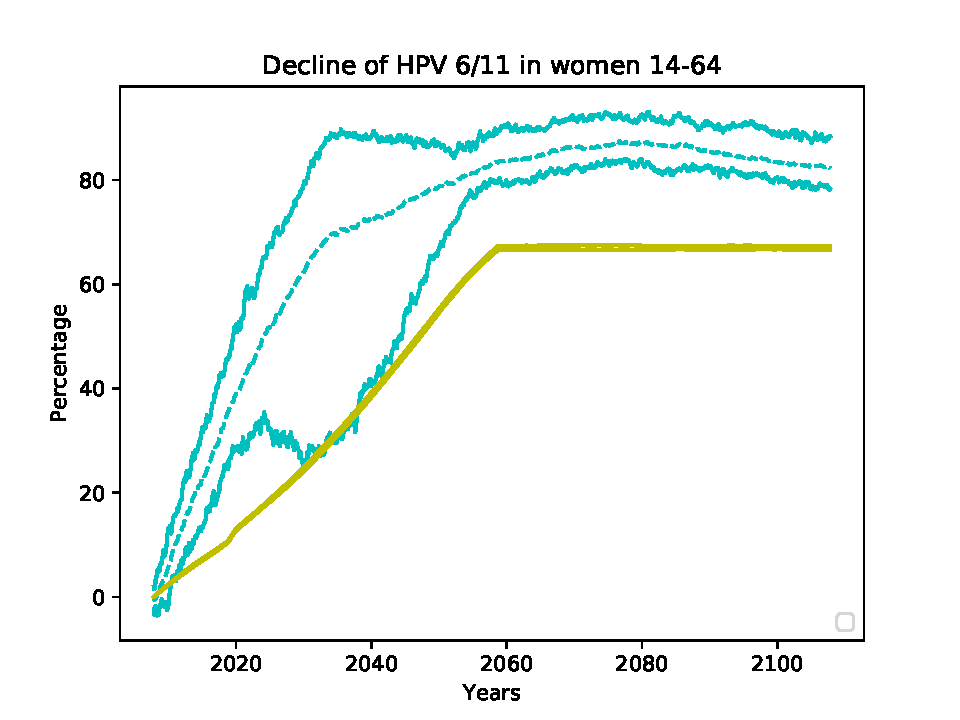
\includegraphics[width=0.5\linewidth]{IMGs/4.-Decline_verrugas/verr_muj.pdf}	& 
		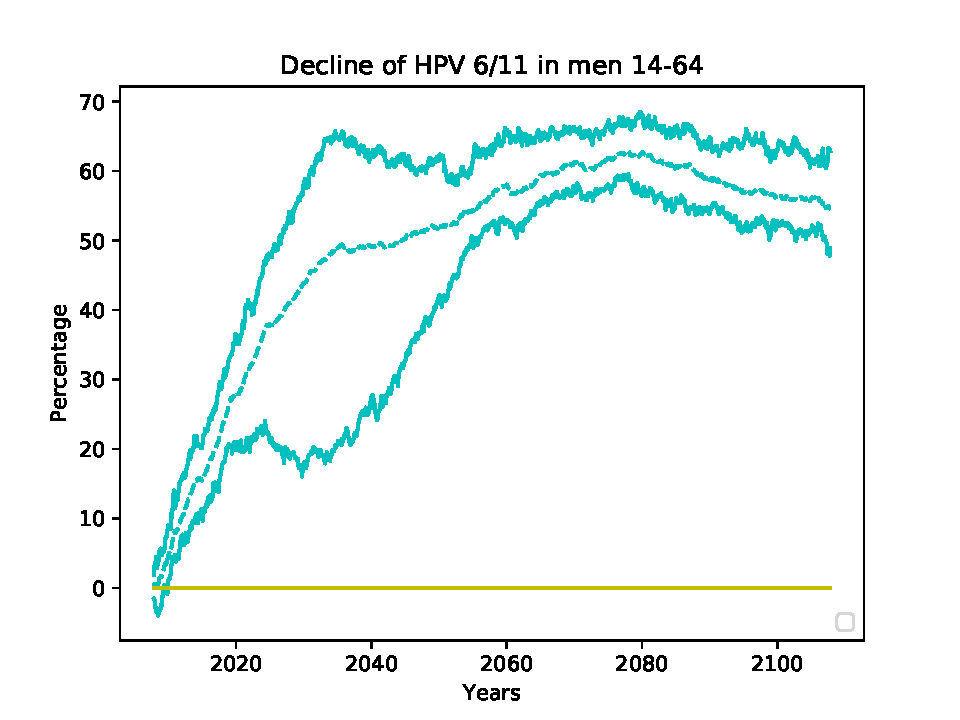
\includegraphics[width=0.5\linewidth]{IMGs/4.-Decline_verrugas/verr_hom.pdf}  \\ 
		(a)	& (b) \\ 
		\multicolumn{2}{c}{ 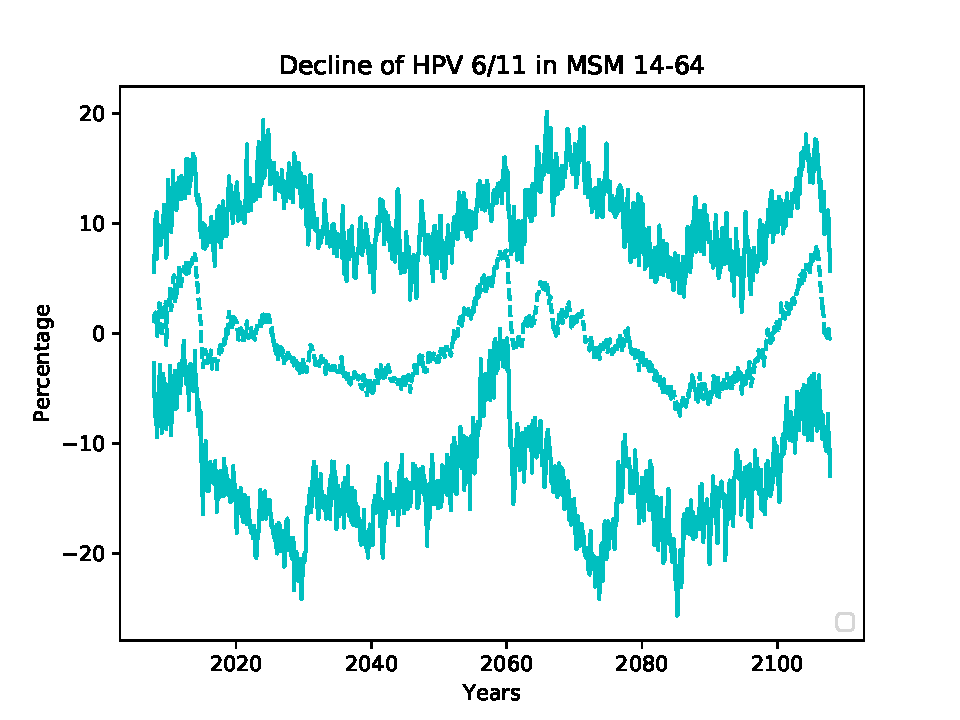
\includegraphics[width=0.5\linewidth]{IMGs/4.-Decline_verrugas/verr_MSM.pdf} } \\ 
		\multicolumn{2}{c}{(c)} \\ 
	\end{tabular} 
	\caption{Decline of HPV LR 6/11 infections, and consequently, of genital warts (GW) in 14-64 years old women (a), men (b) and MSM (c) over the time, from Oct 2007 when the vaccination campaign started in Spain. In the women decline, we include the percentage of vaccinated women. It helps to visualize the herd immunity effect when the decline line is over the vaccination line. In case of men, the lines over the yellow abscissa line means effect of the herd immunity. However, for the MSM, as in the Australian case, there is not herd immunity effect.}
	\label{fig:verrESP}
\end{figure}

The differences between the best and the worst cases is due to the LSP network structure. We do not know exactly how these networks are and the uncertainty that involves the building of these networks may lead to extreme scenarios. This happens in general and in MSM in particular. Thus, we should say that, in our built networks of $100,000$ nodes, less than $2,000$ are labeled MSM. This figure is very low to state predictions for MSM population with a reliable uncertainty and it may explain why the Figure \ref{fig:verrESP} for MSM has so extreme $95\%$ confidence interval.

In the Table \ref{tabla:verrESP}, we can see when given percentages of decline will be reached for women and men. Note that it is not necessary a long time to achieve high percentages of decline for women and men.

\begin{table}[!h]
\centering
\begin{tabular}{c|ll}
	Decline & Women & Men  \\ 
	\hline 
$ 30 \%$ & year  2017 , CI95\% $[ 2015 , 2035 ]$ & year  2021 , CI95\% $[ 2018 , 2044 ]$  \\
$ 40 \%$ & year  2021 , CI95\% $[ 2017 , 2039 ]$ & year  2027 , CI95\% $[ 2023 , 2049 ]$  \\	
$ 50 \%$ & year  2024 , CI95\% $[ 2020 , 2045 ]$ & year  2044 , CI95\% $[ 2027 , 2103 ]$  \\
$ 60 \%$ & year  2029 , CI95\% $[ 2023 , 2047 ]$ & year  2068 , CI95\% $[ 2055 , - ]$  \\
$ 70 \%$ & year  2035 , CI95\% $[ 2027 , 2052 ]$ & year  $-$ , CI95\% $[ - , - ]$  \\
$ 80 \%$ & year  2053 , CI95\% $[ 2030 , 2101 ]$ & year  $-$ , CI95\% $[ - , - ]$  \\
\end{tabular} 
\caption{In this table we show when given percentages of decline of HPV LR 6/11 will be reached over the time with a $95\%$ confidence interval. The symbol "$-$" means that this percentage is not reached in the simulation period. Note that, in average, high percentages of decline for women and men are achieved very soon.}
\label{tabla:verrESP}
\end{table}


  % Simulaci�n caso espa�ol: decline de oncog�nicos
  % !TeX spellcheck = en_US
\section{Decline of HPV oncogenic HR infections in the long-term in Spain}\label{sec:onco_spain}
Here, we are going to repeat the study done in the previous section corresponding to HPV oncogenic HR 16/18/31/33/45/52/58, those GARDASIL9 prevents. In this case, the study may give an idea about the future decline of the cases of HPV-related cancer, but taking into account that cancer use to appear after around $20$ years of persistent infection. 

As in the previous section, we are going to use the procedure explained in Section \ref{sec:decline}. The vaccination program started in Oct 2007.

The results can be seen in Figure \ref{fig:oncoESP}. For women, the herd immunity is present, in average, from $2010$ ($2$ years after the starting of the vaccination program). In the worst case, the herd immunity effect in women appears clearly after $39$ years, around $2047$.

In case of men, in average, the herd immunity appears from the very beginning ($0$ years, $2007.75$). As men are not vaccinated, the herd immunity can be visualized if the line is over zero. In the worst case, $2.5$ years ($2010.25$) are necessary to arise the threshold of the herd immunity. As in the previous cases, herd immunity effect does not appear for MSM.

We should note that, for HPV oncoviruses, the evolution of the decline is more uncertain than for HPV 6/11 after some years of vaccination campaign (see the confidence intervals). Then, if we want to predict when there will be a reduction of cases of cervical cancer after 2030, it may have a delay that could be of 15 years, in the worst case, although the average suggests very promising reductions.

\begin{figure}[!]
	\centering
	\begin{tabular}{cc}
		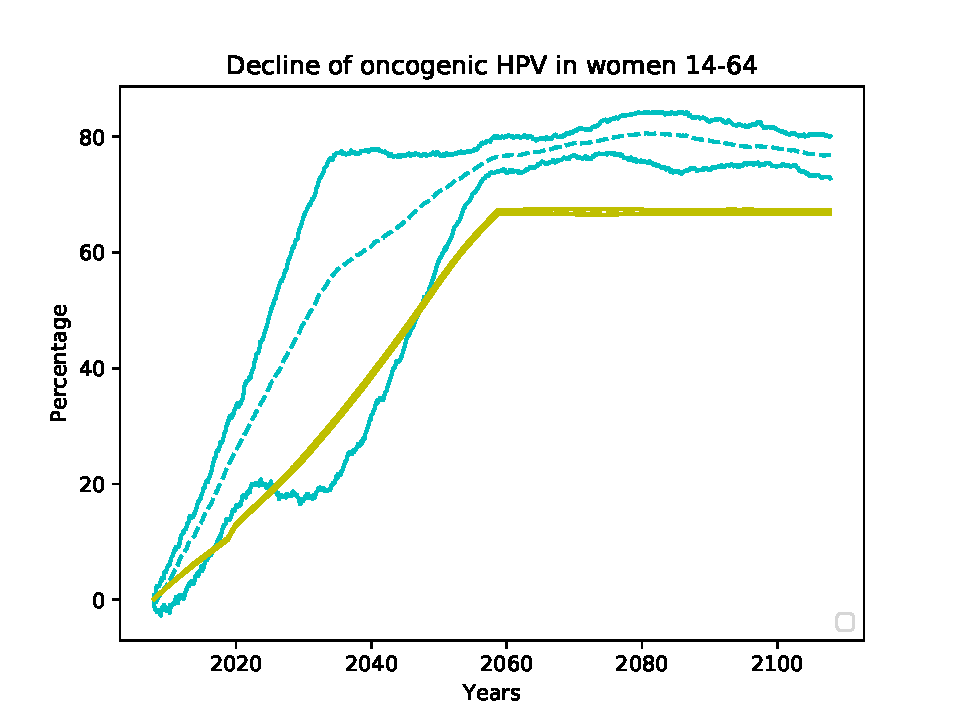
\includegraphics[width=0.5\linewidth]{IMGs/5.-Decline_onco/onco_muj.pdf}	& 
		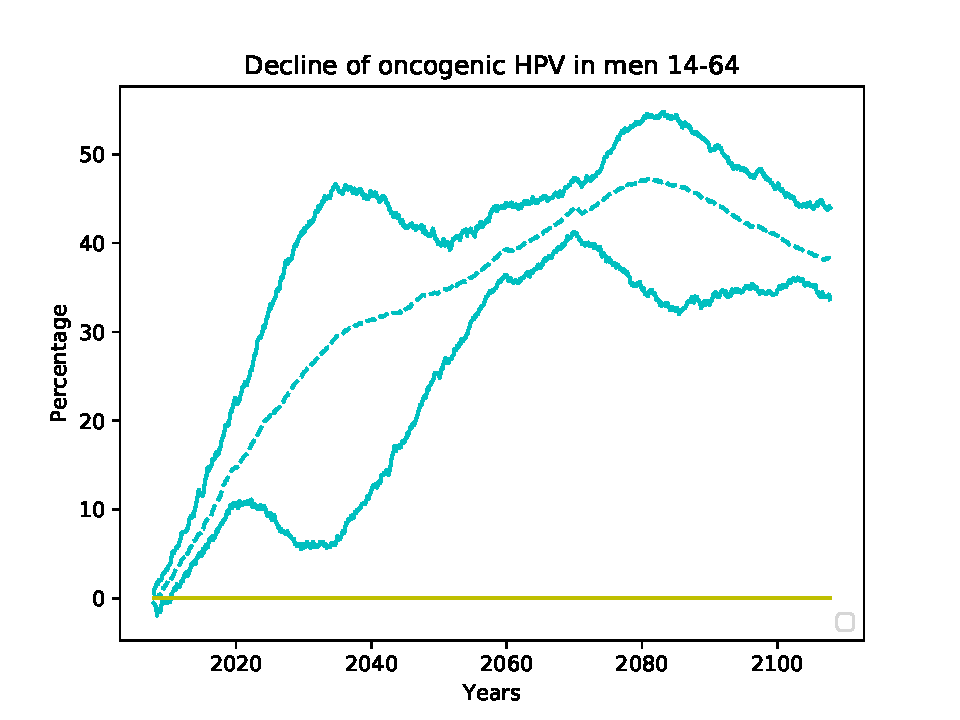
\includegraphics[width=0.5\linewidth]{IMGs/5.-Decline_onco/onco_hom.pdf}  \\ 
		(a)	& (b) \\ 
		\multicolumn{2}{c}{ 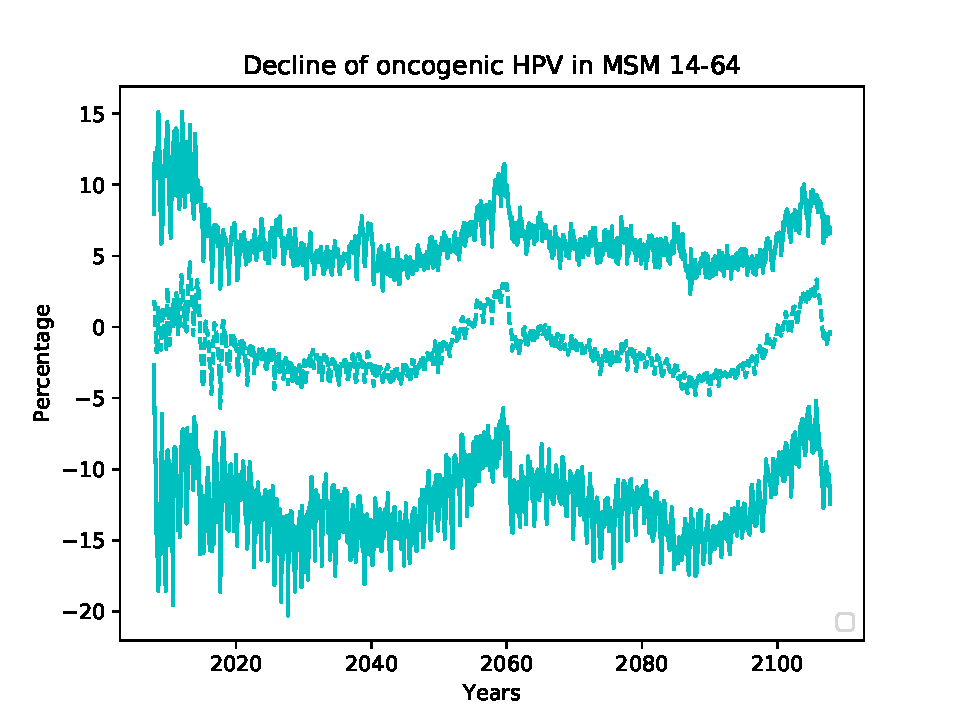
\includegraphics[width=0.5\linewidth]{IMGs/5.-Decline_onco/onco_MSM.pdf} } \\ 
		\multicolumn{2}{c}{(c)} \\ 
	\end{tabular} 
	\caption{Decline of HPV oncogenic HR infections in 14-64 years old women, men and MSM over the time, from Oct 2007, when the vaccination campaign started in Spain. In the women decline, we include the percentage of vaccinated women. It helps to visualize the herd immunity effect when the decline line is over the vaccination line. In case of men, the lines over the yellow abscissa line means effect of the herd immunity. For the MSM, there is not herd immunity effect.}
	\label{fig:oncoESP}
\end{figure}

In the Table \ref{tabla:oncoESP}, we can see when given percentages of decline of HPV oncogenic HR will be reached for women and men. As in the HPV LR case, it is not necessary a long time to achieve high percentages of decline for women and men in average. Furthermore, the decline percentages for oncogenic HPV types are worse than HPV LR 6/11.

\begin{table}[!h]
	\centering
	\begin{tabular}{c|ll}
		Decline & Women & Men \\ 
		\hline 
$ 30 \%$ & year 2022, CI95\% $[ 2019 , 2040 ]$ & year 2036, CI95\% $[ 2024 , 2054 ]$  \\
$ 40 \%$ & year 2027, CI95\% $[ 2023 , 2044 ]$ & year 2063, CI95\% $[ 2029 , 2065 ]$  \\
$ 50 \%$ & year 2031, CI95\% $[ 2025 , 2047 ]$ & year $-$, CI95\% $[ - , - ]$  \\
$ 60 \%$ & year 2039, CI95\% $[ 2028 , 2051 ]$ & year $-$, CI95\% $[ - , - ]$  \\
$ 70 \%$ & year 2050, CI95\% $[ 2032 , 2055 ]$ & year $-$, CI95\% $[ - , - ]$  \\
$ 80 \%$ & year 2076, CI95\% $[ 2058 , - ]$ & year $-$, CI95\% $[ - , - ]$  \\
    \end{tabular} 
	\caption{In this table we show when given percentages of oncogenic HPV decline in Spain with the current vaccination program will be reached over the time with a $95\%$ confidence interval. The symbol "$-$" means that this percentage is not reached in the simulation period. }
	\label{tabla:oncoESP}
\end{table}


  % Simulaci�n caso espa�ol: caida total de la protecci�n tras 20 a�os
  \section{What would happen in Spain if, after 20 years of the vaccination, the effect of the vaccine disappear completely?}
In this section, we are going to simulate what would happen if the vaccine is protecting completely the vaccinated woman during $20$ years and suddenly, in the month after these $20$ year, she losses completely the protection and she becomes vulnerable to the HPV LR 6/11 and HPV oncogenic HR. In Figure \ref{fig:perdida_proteccion} we can see the evolution of the protection simulated for every vaccinated woman.

\begin{figure}[h!]
	\centering
	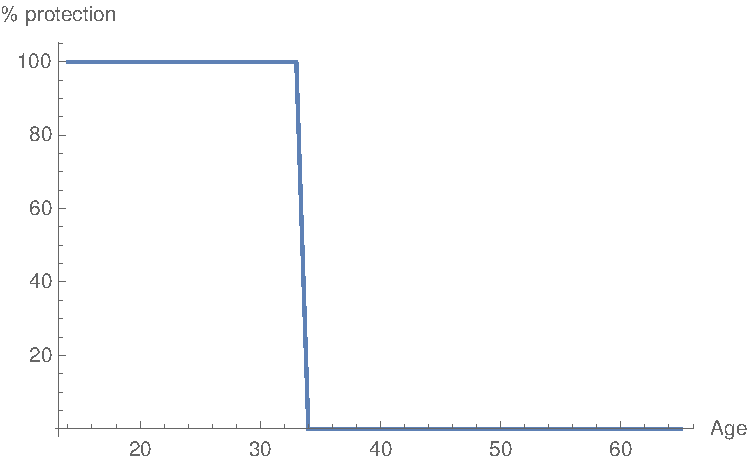
\includegraphics[width=0.5\linewidth]{IMGs/6.-Caida_brusca/grafica_perdida_proteccion.pdf}
	\caption{Evolution of the vaccine protection for every vaccinated woman. After vaccination until $20$ years, the vaccine protects completely ($100\%$) but the month after, the protection drops to $0\%$, the vaccine does not protect anymore.}
	\label{fig:perdida_proteccion}
\end{figure}

In Figure \ref{fig:dropLRESP}, we can see a comparative of the decline of HPV LR 6/11 between the scenario where the effect of the vaccine is permanent and the scenario where the effect of the vaccine disappear completely after $20$ years. In the graphs for women and men we can see how this latter case stabilizes in levels of decline around $20\%$ lower, in average, than the case where the effect of the vaccine is permanent. However, a significant fraction of the population remains protected despite the lost of the protection. Nevertheless, we conjecture that the level of decline in case of protection lost will increase as the time of vaccine protection increases. 

In regard to MSM, we can see that the lost of the vaccine protection does not affect the decline. This is a fact that also supports the statement that there is not herd immunity for MSM, even if the properties of the vaccine change, because the MSM decline does not change.

\begin{figure}[!]
	\centering
	\begin{tabular}{cc}
		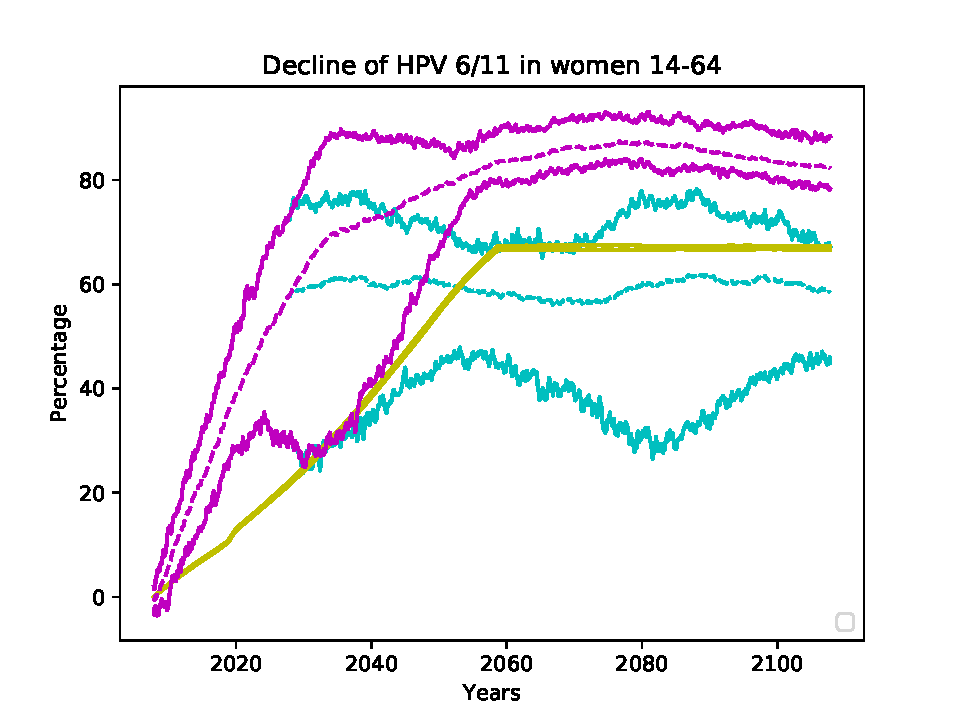
\includegraphics[width=0.5\linewidth]{IMGs/6.-Caida_brusca/verr_muj.pdf}	& 
		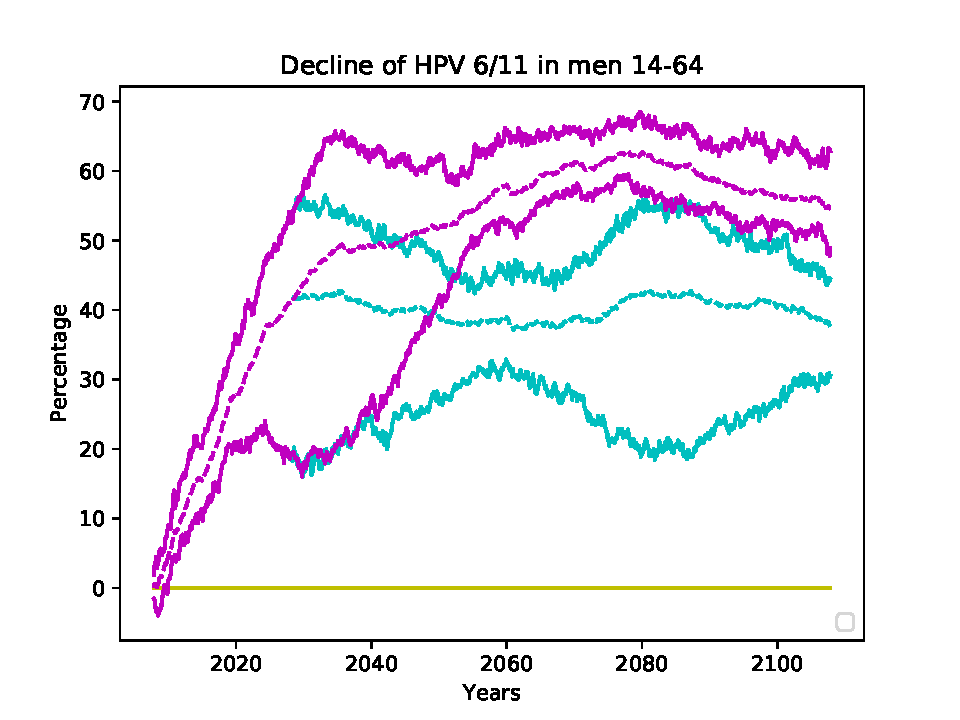
\includegraphics[width=0.5\linewidth]{IMGs/6.-Caida_brusca/verr_hom.pdf}  \\ 
		(a)	& (b) \\ 
		\multicolumn{2}{c}{ 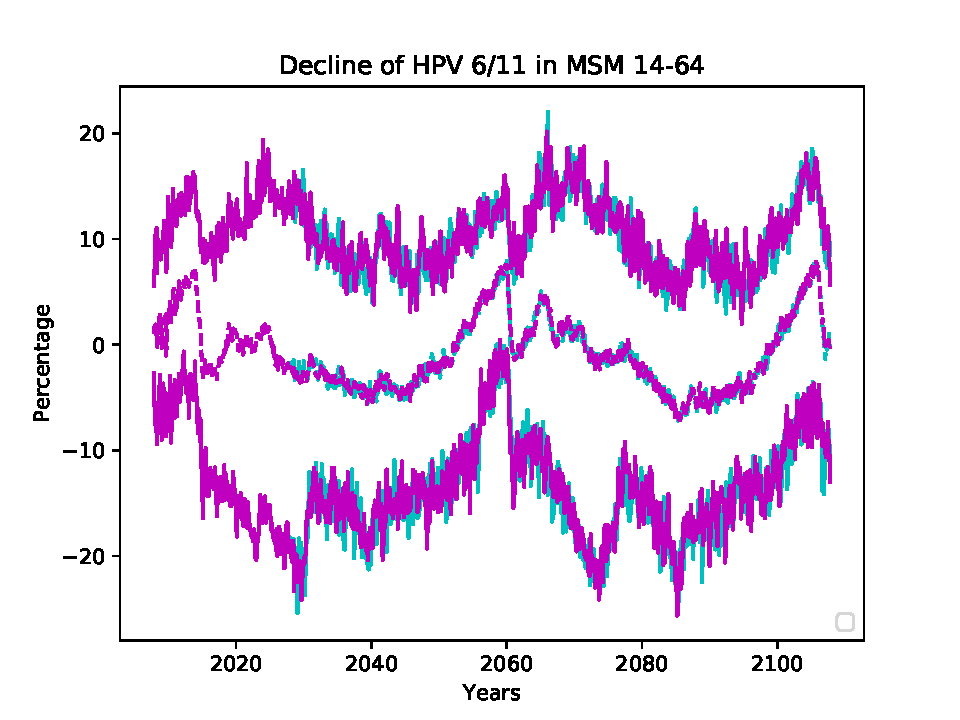
\includegraphics[width=0.5\linewidth]{IMGs/6.-Caida_brusca/verr_MSM.pdf} } \\ 
		\multicolumn{2}{c}{(c)} \\ 
	\end{tabular} 
	\caption{Comparative of the decline of HPV LR 6/11 in 14-64 years old women (a), men (b) and MSM (c) over the time, between the scenario where the effect of the vaccine is permanent (magenta lines, representing  the mean and the $95\%$ confidence interval) and the scenario where the effect of the vaccine disappear completely after $20$ years (cyan lines, representing  the mean and the $95\%$ confidence interval). As we can see, for women and men, the latter stabilizes in levels of decline about $20\%$ less, in average, than the case where the vaccine protects permanently. For MSM there are not changes between both scenarios.}
	\label{fig:dropLRESP}
\end{figure}

Now, in Figure \ref{fig:dropHRESP}, we can see an analogous comparative for the decline of HPV oncogenic HR between the mentioned scenarios: permanent protection and the drop of the protection after $20$ years. The graphs are very similar to the ones in Figure \ref{fig:dropLRESP} with the only change that the difference between the levels of decline are higher. The results for MSM are almost identical, what supports that there is not herd immunity effect on them.

\begin{figure}[!]
	\centering
	\begin{tabular}{cc}
		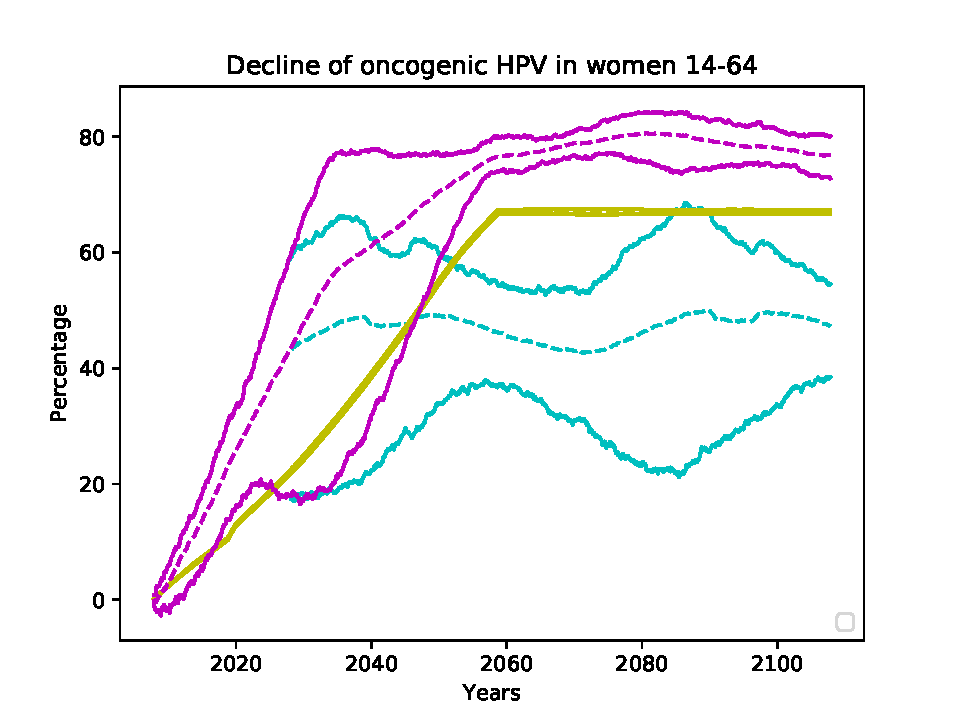
\includegraphics[width=0.5\linewidth]{IMGs/6.-Caida_brusca/onco_muj.pdf}	& 
		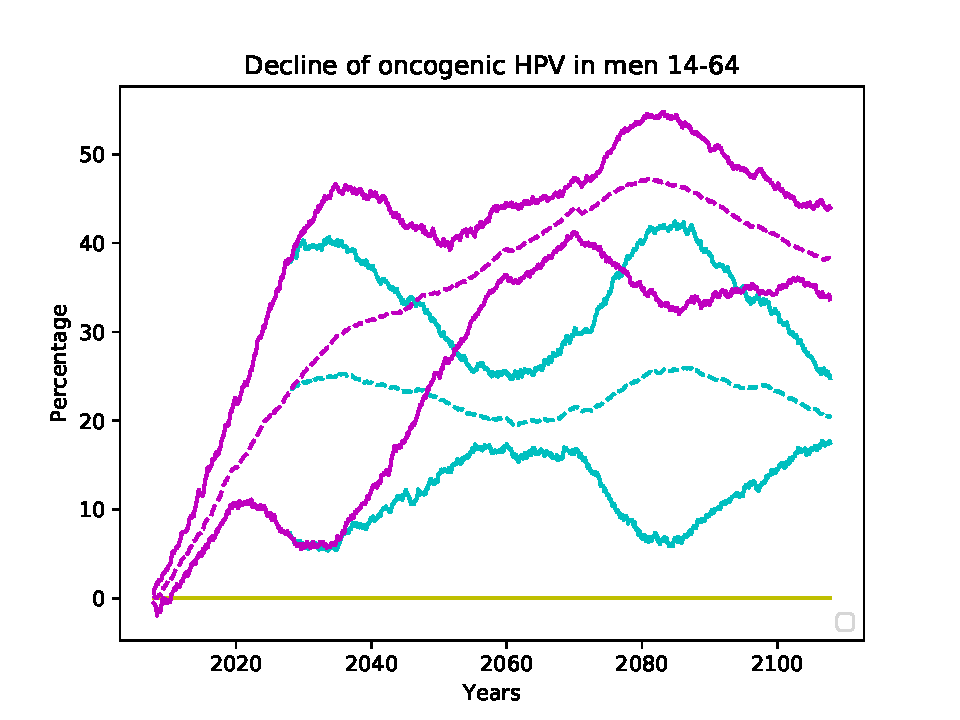
\includegraphics[width=0.5\linewidth]{IMGs/6.-Caida_brusca/onco_hom.pdf}  \\ 
		(a)	& (b) \\ 
		\multicolumn{2}{c}{ 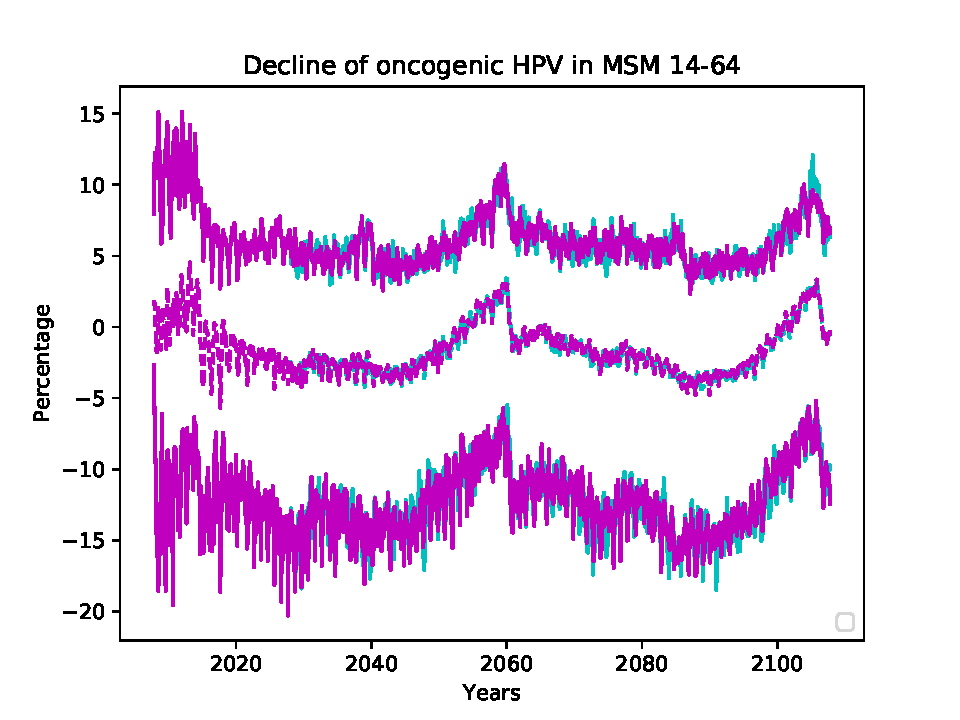
\includegraphics[width=0.6\linewidth]{IMGs/6.-Caida_brusca/onco_MSM.pdf} } \\ 
		\multicolumn{2}{c}{(c)} \\ 
	\end{tabular} 
	\caption{Comparative of the decline of  HPV oncogenic HR infections in 14-64 years old women (a), men (b) and MSM (c) over the time, between the scenario where the effect of the vaccine is permanent (magenta lines, representing  the mean and the $95\%$ confidence interval) and the scenario where the effect of the vaccine disappear completely after $20$ years (cyan lines, representing  the mean and the $95\%$ confidence interval). The graphs are very similar to the ones in Figure \ref{fig:dropLRESP} with the only change that the difference between the levels of decline are higher. For MSM there are not changes between both scenarios.}
	\label{fig:dropHRESP}
\end{figure}

Now, we are going to perform a sensitivity analysis, consisting of the comparison between the decline of HPV infection if there is a drop in the vaccine protection after 20 years and after 30 years. This comparison will be done only for men and women, because there are not differences in MSM because there is not herd immunity effect on the MSM. The results can be seen in Figure \ref{fig:compara_caida}.

\begin{figure}[!]
	\centering
	\begin{tabular}{cc}
		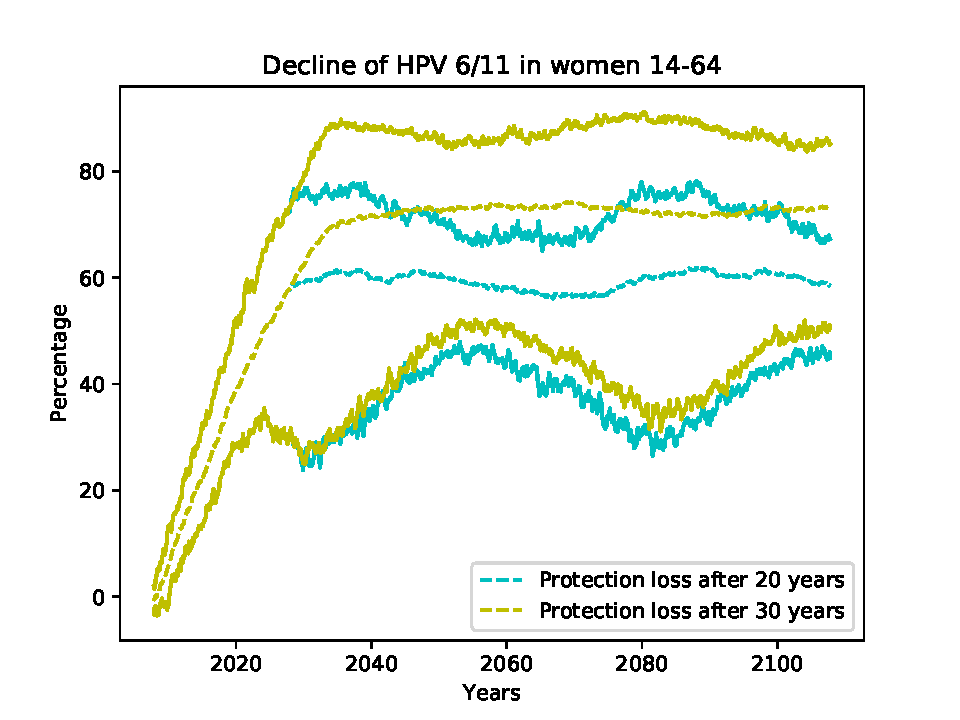
\includegraphics[width=0.5\linewidth]{IMGs/7.-Compara_caida/verr_muj.pdf}	& 
		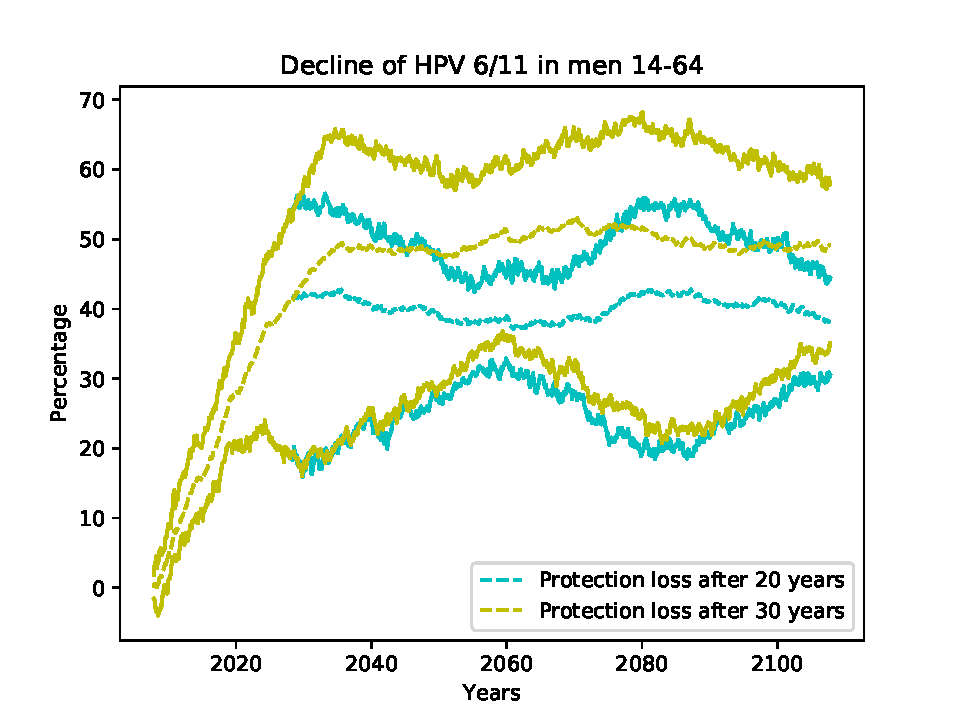
\includegraphics[width=0.5\linewidth]{IMGs/7.-Compara_caida/verr_hom.pdf}  \\ 
		(a)	& (b) \\ 
		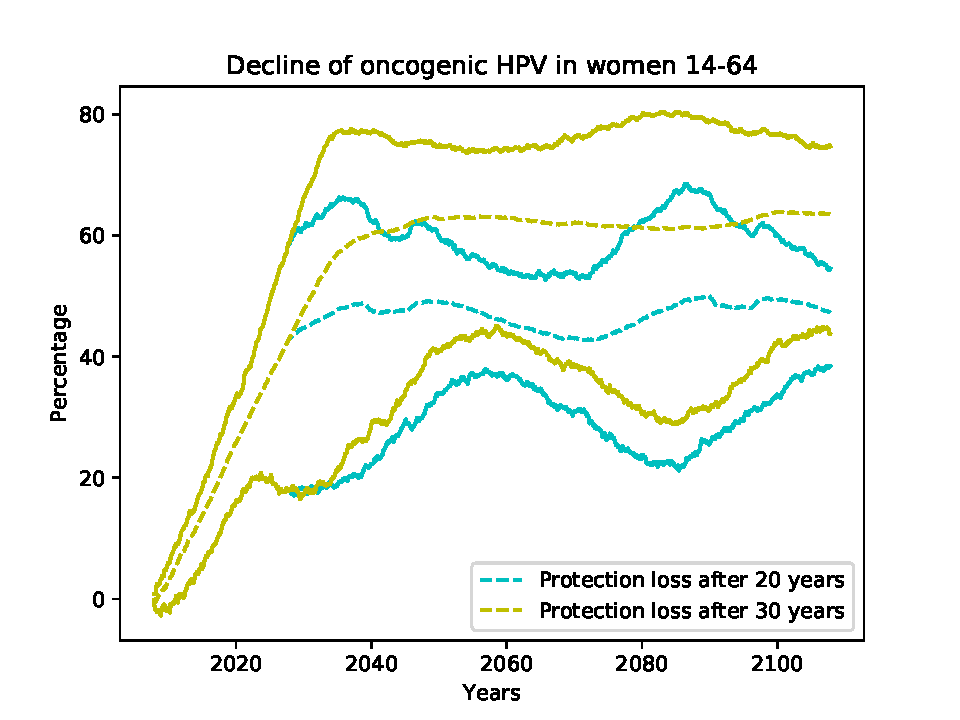
\includegraphics[width=0.5\linewidth]{IMGs/7.-Compara_caida/onco_muj.pdf}	& 
		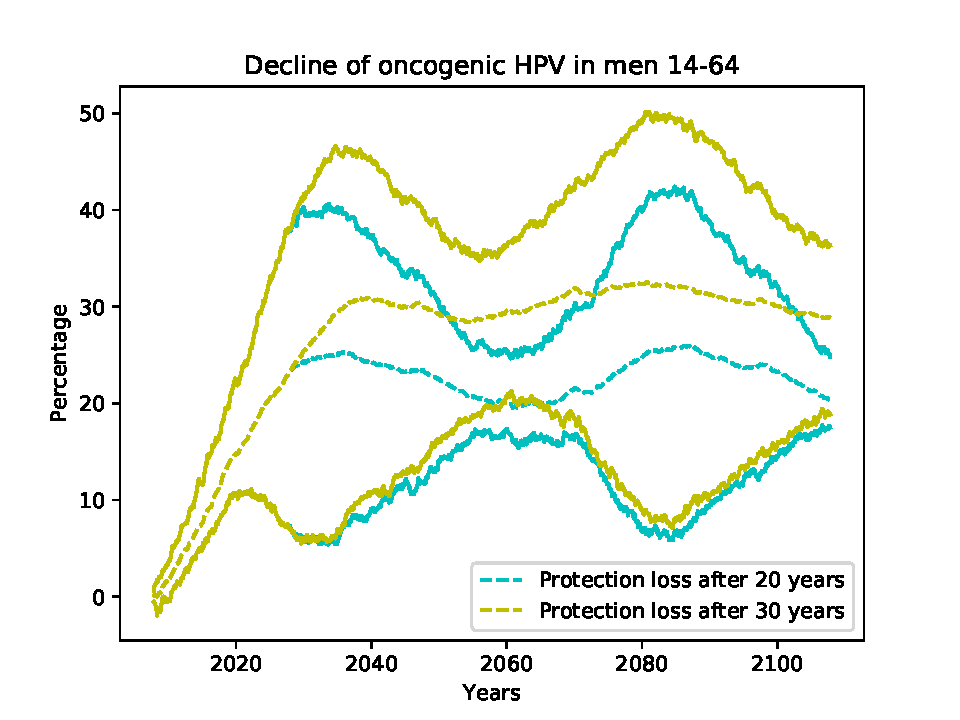
\includegraphics[width=0.5\linewidth]{IMGs/7.-Compara_caida/onco_hom.pdf}  \\ 
		(c)	& (d) \\ 
	\end{tabular} 
	\caption{Comparative of the decline of HPV 6/11 infections in 14-64 years old women (a) and men (b) over the time, between the scenario where the drop of the vaccine protection occurs after 20 years of vaccination (cyan lines) and after 30 years (yellow lines). The same for figures (c) and (d) with HPV oncogenic infection. The difference of 10 years in the drop results in around $10\%$ of difference in the decline.}
	\label{fig:compara_caida}
\end{figure}

Figure \ref{fig:compara_caida} leads us to conclude that the longer is the vaccine protection the lower will be the drop in the decline. 

To finish the present section, we are going to show Figure \ref{fig:proteccion} where we can see the percentage of women protected by the vaccine if the protection is permanent and if there is a loss of protection after 20 and 30 years.

\begin{figure}[!]
	\centering
	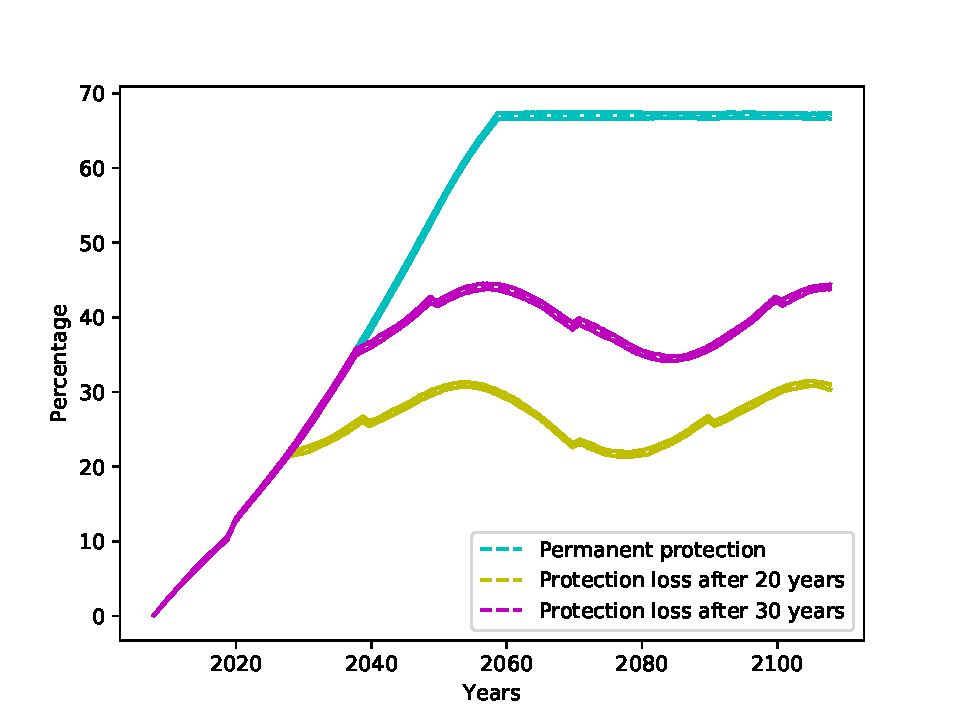
\includegraphics[width=0.5\linewidth]{IMGs/7.-Compara_caida/proteccion_muj.pdf}	
	\caption{Percentage of women protected by the vaccine in three scenarios: permanent protection (cyan line), total loss of protection after 30 years (magenta line) and total loss of protection after 20 years (yellow line).}
	\label{fig:proteccion}
\end{figure}


  % Simulaci�n caso espa�ol: turismo
  \section{Simulation of the effect of the tourism on the contagion of HPV in Spain}
In $2017$, $82$ millions of tourists visited Spain \cite{INEturismo}. These visits may have influence on the spread of HPV and this is what we are going to study in the present section.

Unfortunately, there are not available data related to the number of infections due to sexual intercourses with tourists, therefore, we are going to introduce a more or less believable scenario, skewing a bit against the vaccine. This scenario will simulate, every month, that $1\%$ of Spanish individuals aged $18-29$ years old with $4$ or more LSP have sexual intercourses with infected tourists.

To do so, we need to introduce a new feature in the computational model to simulate the effect of the tourism. First, recall that, following \cite{castellsague2012prevalence}, among the infected women, $76.03\%$ of them are infected of HPV HR, $11.72\%$ are infected of HPV LR and $12.24\%$ are infected by both, HR and LR. Also, $50.35\%$ of the HPV HR are with oncogenic types, that is, HPV 16/18/31/33/45/52/58. Furthermore, $37.075\%$ of the HPV LR are with 6/11. Then, for all individuals with $4$ or more LSP aged $18-29$ ($rnd()$ denotes a computational function that generates a random number in the interval $[0,1]$.

\begin{itemize}
	\item If $rnd()<0.01$ (the individual may be infected by a tourist) and let $x=rnd()$
	\begin{itemize}
		\item If $x < 0.7603$ the node gets infected by HPV HR. Also, if $rnd() < 0.5035$ and the individual is not vaccinated, the infection is by an oncogenic HPV HR.
		\item If $0.7603 \leq x < 0.7603 + 0.1172$ the node gets infected by HPV LR. Also, if $rnd() < 0.3707$ and the individual is not vaccinated, the infection is by HPV 6/11.
		\item If $0.7603 + 0.1172 \leq x $ the node gets infected by HPV LR and by HPV LR (coinfection). Thus, if $rnd() < 0.5035$ and the individual is not vaccinated, the infection is by an oncogenic HPV HR and $rnd() < 0.3707$ the infection is also by HPV 6/11.
	\end{itemize}
\end{itemize}

Including the above features in the computational model and performing a simulation, in the Figure \ref{fig:turismo} we can see the influence of the tourism in the HPV infections.

\begin{figure}[!]
	\centering
	\begin{tabular}{cc}
		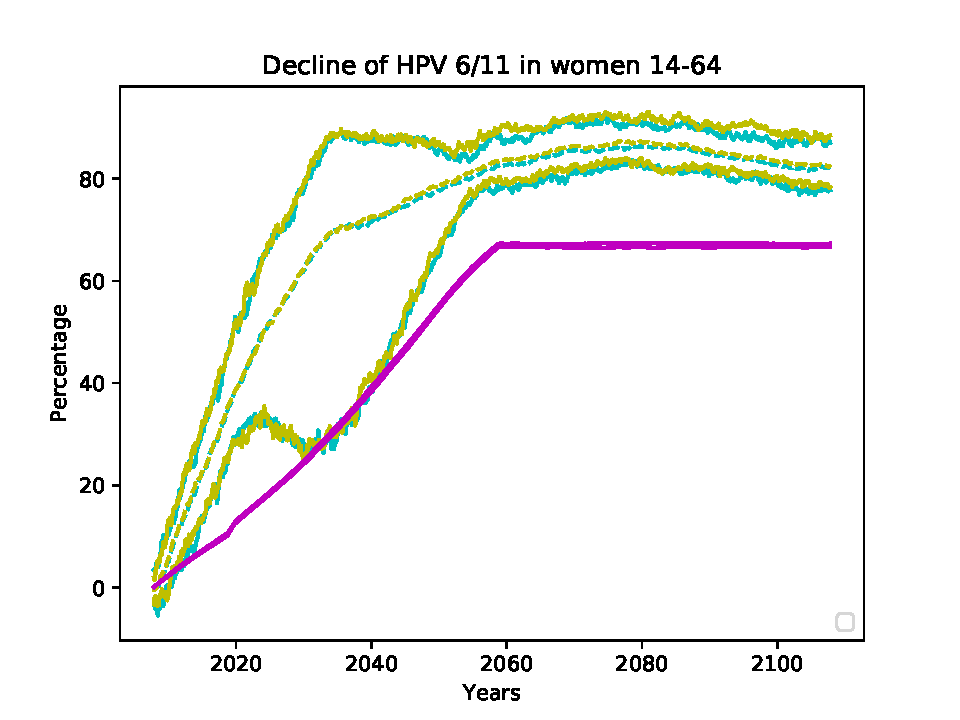
\includegraphics[width=0.5\linewidth]{IMGs/8.-Turismo/verr_muj.pdf}	& 
		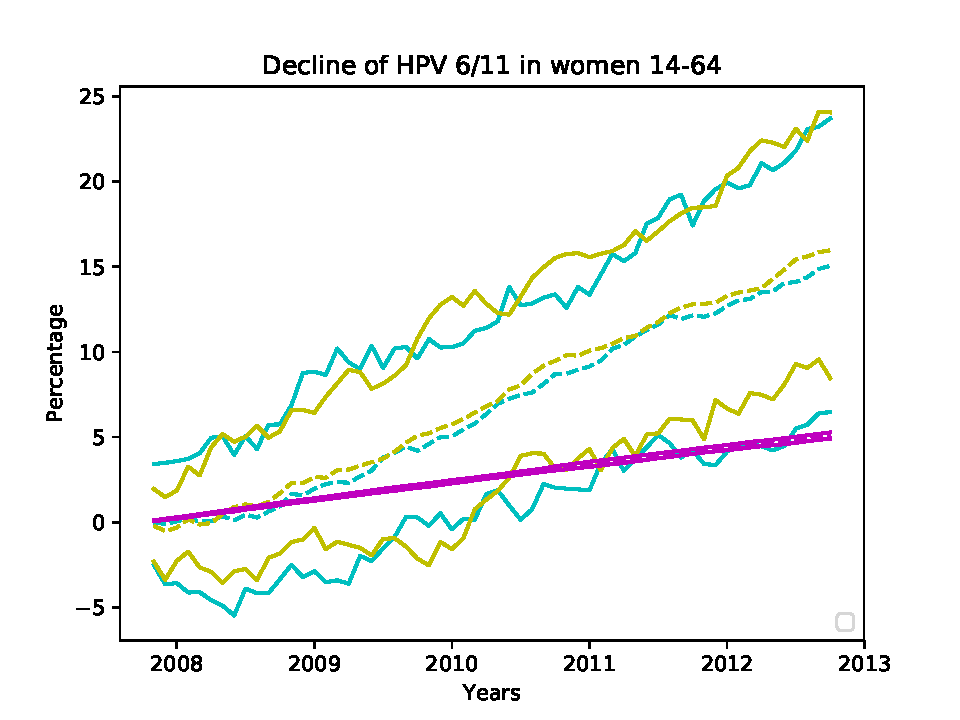
\includegraphics[width=0.5\linewidth]{IMGs/8.-Turismo/verr_muj_ZOOM.pdf}  \\ 
		(a)	& (b) \\ 
		\includegraphics[width=0.5\linewidth]{IMGs/8.-Turismo/verr_hom.pdf}	& 
		\includegraphics[width=0.5\linewidth]{IMGs/8.-Turismo/verr_hom_ZOOM.pdf}  \\ 
		(c)	& (d) \\ 		
		\includegraphics[width=0.5\linewidth]{IMGs/8.-Turismo/verr_MSM.pdf}	& 
		\includegraphics[width=0.5\linewidth]{IMGs/8.-Turismo/verr_MSM_ZOOM.pdf}  \\ 
		(e)	& (f)
 	\end{tabular} 
	\caption{Comparative of the decline of  HPV LR 6/11 in 14-64 years old women (a), men (c) and MSM (e) over the time and a zoom of the graphs for the first five years for women (b), men (d) and MSM (f), between the non-tourism scenario (yellow lines) and the tourism scenario where every month $1\%$ of Spanish individuals aged $18-29$ years old with $4$ or more LSP have sexual intercourses with infected tourists (cyan lines). Magenta lines show the percentage of vaccinate women and men (nobody in men). No remarkable changes appear.}
	\label{fig:turismo}
\end{figure}

Figure \ref{fig:turismo} shows that there are not remarkable differences between both scenarios including the very beginning, where there are very few girls vaccinated. Therefore, the tourism does not seem to be a factor that influences the decline the HPV 6/11. Here we do not show the same graphs for HPV oncogenic because of their similarity with the ones in Figure \ref{fig:turismo}. 

  % Simulaci�n caso espa�ol: vacunaci�n de ni�os y ni�as para erradicar el c�ncer por VPH
  % !TeX spellcheck = en_US
\section{Simulation of different vaccination strategies in girls and boys with the aim to eradicate the cancer diseases associated HPV oncogenic HR}\label{vaccinationStrategies}
In this Chapter, we are going to simulate the scenarios where we vaccinate GARDASIL9 to boys and girls with a coverage of $60\%$, $75\%$ and $90\%$. Then, we will see when a decline of $65\%$, $75\%$, $85\%$ and $95\%$ is reached in all the cases for HPV oncogenic HR. Our results will be compared with the ones in \cite{Brisson2016}, where the authors consider that the elimination of the HPV HR included in GARDASIL9 (the oncogenic ones) will be reached after $80$ years vaccinating boys and girls with a coverage of $80\%$. The results can be seen in Table \ref{tabla:decline_HR_onco}.

\begin{sidewaystable}[ph!]
	\hspace*{-6em}%me lo saco de la manga de Internet
	\centering
	\small
	\begin{tabular}{c|lll}
        \\
        \hline
        \multicolumn{4}{c}{\textbf{Vaccination of boys and girls with a coverage of $60\%$}}\\
        \hline
        Decline & Women &  Men & MSM \\ 
        \hline		
$ 65 \%$ & year 2040, CI95\% $[ 2029 , 2051 ]$ & year  2047, CI95\% $[ 2031 , 2053 ]$ & year $-$, CI95\% $[ 2053, - ]$ \\
$ 75 \%$ & year 2050, CI95\% $[ 2032 , 2055 ]$ & year  2058, CI95\% $[ 2038, 2070 ]$ & year  $-$, CI95\% $[ - , - ]$ \\
$ 85 \%$ & year 2084, CI95\% $[ 2069, - ]$ & year  $-$, CI95\% $[ - , - ]$ & year  $-$, CI95\% $[ - , - ]$ \\
$ 95 \%$ & year $-$, CI95\% $[ - , - ]$ & year  $-$, CI95\% $[ - , - ]$ & year  $-$, CI95\% $[ - , - ]$ \\
		\\
		\hline 		
		\multicolumn{4}{c}{\textbf{Vaccination of boys and girls with a coverage of $75\%$}}\\
		\hline
		Decline & Women &  Men & MSM \\ 
		\hline 
$ 65 \%$ & year 2034, CI95\% $[ 2028 , 2047 ]$ & year 2039, CI95\% $[ 2028 , 2048 ]$ & year 2045, CI95\% $[ 2042 , 2049 ]$ \\
$ 75 \%$ & year 2042, CI95\% $[ 2030 , 2050 ]$ & year 2046, CI95\% $[ 2032 , 2052 ]$ & year 2053, CI95\% $[ 2049 , 2059 ]$ \\
$ 85 \%$ & year 2050, CI95\% $[ 2033 , 2054 ]$ & year 2054, CI95\% $[ 2042 , 2056 ]$ & year $-$, CI95\% $[ - , - ]$ \\
$ 95 \%$ & year $-$, CI95\% $[ 2060 , - ]$ & year $-$, CI95\% $[ - , - ]$ & year $-$, CI95\% $[ - , - ]$ \\
         \\
         \hline
         \multicolumn{4}{c}{\textbf{Vaccination of boys and girls with a coverage of $90\%$}}\\
         \hline
         Decline & Women &  Men & MSM \\ 
         \hline
$ 65 \%$ & year 2032, CI95\% $[ 2027 , 2046 ]$ & year 2035, CI95\% $[ 2027 , 2046 ]$ & year 2039, CI95\% $[ 2036 , 2042 ]$ \\
$ 75 \%$ & year 2038, CI95\% $[ 2029 , 2050 ]$ & year 2041, CI95\% $[ 2030 , 2049 ]$ & year 2044, CI95\% $[ 2041 , 2047 ]$ \\
$ 85 \%$ & year 2046, CI95\% $[ 2032 , 2052 ]$ & year 2048, CI95\% $[ 2033 , 2052 ]$ & year 2050, CI95\% $[ 2047 , 2052 ]$ \\
$ 95 \%$ & year 2054, CI95\% $[ 2042 , 2056 ]$ & year 2055, CI95\% $[ 2048 , 2057 ]$ & year $-$, CI95\% $[ 2056 , - ]$
	\end{tabular} 
	\caption{Here, we show when a decline of HPV oncogenic HR of $65\%$, $75\%$, $85\%$ and $95\%$ is reached when vaccinating boys and girls with a coverage of $60\%$, $75\%$ and $90\%$. MSM are included in men, and also considered separately.}
	\label{tabla:decline_HR_onco}
\end{sidewaystable}

Now, in Figure \ref{fig:erradicacion}, we show some graphs about the decline of HPV oncogenic in 14-64 years old women, men and MSM with coverage for women and men of $75\%$ and $90\%$. The difference between the percentage of vaccinated individuals (yellow lines) and the decline of the HPV (cyan lines) is a measure of the herd immunity effect on each population. As we can see, the herd immunity effect on women and men are similar. The small differences are because men include MSM even though the percentage of MSM is low respect to the total of men. Nevertheless, in MSM, the herd immunity is low, because their high number of LSP that MSM have.  

\begin{figure}[!]
	\centering
	\begin{tabular}{cc}
		\includegraphics[width=0.5\linewidth]{IMGs/9.-Erradicacion_ONCO/onco_muj_75.pdf}	& 
		\includegraphics[width=0.5\linewidth]{IMGs/9.-Erradicacion_ONCO/onco_muj_90.pdf}  \\ 
		Decline. Women. Coverage $75\%$	& Decline. Women. Coverage $90\%$ \\ 
		\includegraphics[width=0.5\linewidth]{IMGs/9.-Erradicacion_ONCO/onco_hom_75.pdf}	& 
		\includegraphics[width=0.5\linewidth]{IMGs/9.-Erradicacion_ONCO/onco_hom_90.pdf}  \\ 
		Decline. Men. Coverage $75\%$	& Decline. Men. Coverage $90\%$ \\ 		
		\includegraphics[width=0.5\linewidth]{IMGs/9.-Erradicacion_ONCO/onco_MSM_75.pdf}	& 
		\includegraphics[width=0.5\linewidth]{IMGs/9.-Erradicacion_ONCO/onco_MSM_90.pdf}  \\ 
		Decline. MSM. Coverage $75\%$	& Decline. MSM. Coverage $90\%$
	\end{tabular} 
	\caption{Decline of HPV oncogenic in 14-64 years old women, men and MSM with coverage for women and men of $75\%$ and $90\%$ over the time. The horizontal dashed lines point out the decline percentages of $65\%$, $75\%$, $85\%$ and $95\%$. The difference between the cyan and the yellow lines is a measure of the herd immunity effect on each population. In this case, due to the high coverage, we can see herd immunity effect in MSM only in the long-run.}
	\label{fig:erradicacion}
\end{figure}

As we can see in the Figure \ref{fig:erradicacion}, the highest values of decline are reached around $2060$ in all the graphs, that is, after a complete generation has been vaccinated. Therefore, a high coverage for women and men during a whole generation has to be considered if we want to eradicate the cancer produced by HPV oncogenic. 

Nevertheless, Figure \ref{fig:erradicacion} shows that the variation of the decline in the long-run between the vaccination of $75\%$ to $90\%$ is small if we think that we need an increase of $15\%$ in coverage. From year $2060$ to $2100$, the differences in the decline between coverage $90\%$ and $75\%$ are: in men vary from $6.3\%$ to $10.1\%$; in women vary from $3.3\%$ to $6.4\%$; and for MSM vary from $10.2\%$ to $20\%$. Only in the MSM coverage increase is fully reflected in the similar order of magnitude, around $15\%$. In other words, looking at Table \ref{tabla:decline_HR_onco}, with the increase in the coverage from $75\%$ to $90\%$, in average, the levels of decline $65\%$, $75\%$ and $85\%$ are reached $2 - 4$ years before for women and $4 - 6$ years before for men. For MSM, the levels of decline $65\%$ and $75\%$ are reached $6 – 9$ years before, in average. This fact may suggest that, reaching coverages around $70\% - 75\%$ is enough to have a high protection in the whole population without a significant increasing of the vaccination cost to achieve small increases in the decline in the long-run.

Also, we would like to point out that the herd immunity effect, measured by the difference between the decline lines (cyan) and the vaccination lines (yellow), is similar in men and women, and there is a small herd immunity in MSM in the long-run, due to the high vaccine coverage.

In recent papers as \cite{Brisson2016, SIMMS2019394, BRISSON2019319}, the authors find possible the elimination of the oncogenic HPV included in GARDASIL9 in around a generation. However, our model with its accurate replication of the herd immunity effect, suggests that we have to be cautious. MSM have small herd immunity effect and, therefore, if we are not able to vaccinate almost all the MSM with higher coverages on them, the unprotected MSM may preserve the circulation of the virus due to their high number of sexual partners. 

  
  % Simulaci�n caso espa�ol: estudio de resilencia
  \section{Quantifying the delay to recover normal levels of decline due to a drop in the vaccination coverage}\label{Resilence}
In Denmark, the vaccination program started in $2009$ with a coverage of $80\%$. After $5$ years, in $2$ months the coverage dropped until $10\%$. It remained $2$ years in $10\%$ and then, in $5$ years increased until $70\%$ and remained constant. In Figure \ref{fig:cobertura_danesa} we show the coverage evolution. 

\begin{figure}[h!]
	\centering
	\includegraphics[width=0.5\linewidth]{IMGs/11.-Resilencia/Cobertura_Danesa.pdf}
	\caption{Evolution of the HPV vaccine coverage from the program starting in 2009.}
	\label{fig:cobertura_danesa}
\end{figure}

Drops in the coverage have happened in some countries and it is a concerning issue because the natural consequence is the delay in achieving high rates of protection (resilence) in order to reduce the pathologies associated to HPV.

Thus, here, we are going to perform simulations to study the delay produced due to a drop in the coverage under different circumstances. A first approach has published in \cite{Elfstrm2015}, where the authors consider an age-structured model of differential equations \cite{Baussano2013} to simulate the following vaccination programs

\begin{enumerate}
	\item Case 1 or base case: vaccination of $80.5\%$ girls aged 11-12 and $53.25\%$ of the girls aged 13-18.
	\item Case 2: base case $+$ vaccination of $80.50\%$ of women aged 22-26 during the year 2015.
	\item Case 3: Case 2 $+$ vaccination of $80.50\%$ of the boys aged 11-12.
	\item Case 4: Case 3 $+$ vaccination of $80.50\%$ of the boys aged 13-26 during the year 2015.
\end{enumerate}

The above strategies are consistent with the Swedish policies, where they started vaccinating girls since 2007. The authors assume a vaccination effectiveness of $95\%$ in the vaccination of 11-12 years old boys and girls and $92\%$ for older ones.

The results obtained in \cite{Elfstrm2015} say that the vaccination programs are more resilent when only girls are vaccinate, that is, the effect of a drop in the coverage is greater if only girls are vaccinated because the decline in HPV infection is recovered faster if boys and girls are vaccinated. Also, they say that \textit{if vaccination coverage is high, $25-30$ years after vaccination commences, the effectiveness converges. The most salient impact of male vaccination is the mitigation of loss of vaccine effectiveness in the face of an unexpected reduction in coverage}.

Our goal here is to see if using our model and scenarios adapted to the Spanish situation, we are able to obtain similar results to the those in \cite{Elfstrm2015}. In our case, we propose the following scenarios

\begin{enumerate}
	\item Case 1 or base case: vaccination of $14$ years old girls with a coverage of $70\%$ starting in $2008$ (current situation in Spain).
	\item Case 2: base case $+$ vaccination of $14$ years old boys with a coverage of $70\%$ starting in January $2020$.
	\item Case 3: base case $+$ in January $2025$, in $2$ months the coverage drops until $10\%$, it remains $2$ years in $10\%$ and then, in $5$ years increases until $70\%$ and remains constant (Danish scenario).
	\item Case 4: Case 2 $+$ Danish scenario starting in January 2025 droping the coverage in boys and girls (Danish scenario for both boys and girls).
\end{enumerate}

Here, we assume an effectiveness of $96.5\%$ and the use of Gardasil9. We do not have scenarios with catchup vaccination, because in \cite{Skufca}, as we mentioned previously, the authors performs a literature review where they show that the effectiveness of the HPV vaccine on cervical abnormalities is between $20\% − 54\%$ instead of the assumed $96.5\%$ or $92\%$ assumed in \cite{Elfstrm2015}. Recall that we performed a simulation with the data appearing in \cite{Skufca} in Section \ref{sec:australia_sfuka} in page \pageref{sec:australia_sfuka} and we conclude that the catch-up effectiveness may be higher than the figures collected in \cite{Skufca} but far from $92\%$. Thus, it seems to be clear that the vaccine effectiveness experiments a reduction in those women who had previous contact with the virus.

In order to study the resilence, we are going to compare the delay produced in the decline of infections between, on the one hand, the Base Case and the Case 3 (only girls vaccination), and on the other hand, the Case 1 and the Case 4 (vaccination of boys ans girls).  

We show the obtained results in Figures \ref{fig:baseCase_Case3} and \ref{fig:Case2_Case4}. Figure \ref{fig:baseCase_Case3} depicts the comparison between the Base Case and the Case 3 and Figure \ref{fig:Case2_Case4} the comparison between the Case 2 and the Case 4. In both figures, on the left column we can see the evolution over the time of the average decline of the oncogenic HPV in men, MSM and women, from year $2025$ (when the drop starts). On the right column, we visualize the average number of years the simulation with the drop in the coverage needs to achieve the same level of decline as the simulation without drop, from year $2025$ until $2055$.

\begin{figure}[!]
	\centering
	\begin{tabular}{cc}
		\includegraphics[width=0.5\linewidth]{IMGs/11.-Resilencia/Base_y_3/decline_onco_hom.pdf}	& 
		\includegraphics[width=0.5\linewidth]{IMGs/11.-Resilencia/Base_y_3/resilencia_onco_hom.pdf}  \\ 
		(a)	& (b) \\ 
		\includegraphics[width=0.5\linewidth]{IMGs/11.-Resilencia/Base_y_3/decline_onco_MSM.pdf}	& 
		\includegraphics[width=0.5\linewidth]{IMGs/11.-Resilencia/Base_y_3/resilencia_onco_MSM.pdf}  \\ 
		(c)	& (d) \\
		\includegraphics[width=0.5\linewidth]{IMGs/11.-Resilencia/Base_y_3/decline_onco_muj.pdf}	& 
		\includegraphics[width=0.5\linewidth]{IMGs/11.-Resilencia/Base_y_3/resilencia_onco_muj.pdf}  \\ 
		(e)	& (f) \\  
	\end{tabular} 
	\caption{Comparative of Base Case and Case 3. On the left column, the average decline of oncogenic HPV in men (a), MSM (c) and women (e), in both cases. On the right column, the time (in years) the Case 3 needs to achieve the same levels of decline as the Base Case for oncogenic HPV in men (b), MSM (d) and women (f).}
	\label{fig:baseCase_Case3}
\end{figure}

\begin{figure}[!]
	\centering
	\begin{tabular}{cc}
		\includegraphics[width=0.5\linewidth]{IMGs/11.-Resilencia/2_y_4/decline_onco_hom.pdf}	& 
		\includegraphics[width=0.5\linewidth]{IMGs/11.-Resilencia/2_y_4/resilencia_onco_hom.pdf}  \\ 
		(a)	& (b) \\ 
		\includegraphics[width=0.5\linewidth]{IMGs/11.-Resilencia/2_y_4/decline_onco_MSM.pdf}	& 
		\includegraphics[width=0.5\linewidth]{IMGs/11.-Resilencia/2_y_4/resilencia_onco_MSM.pdf}  \\ 
		(c)	& (d) \\
		\includegraphics[width=0.5\linewidth]{IMGs/11.-Resilencia/2_y_4/decline_onco_muj.pdf}	& 
		\includegraphics[width=0.5\linewidth]{IMGs/11.-Resilencia/2_y_4/resilencia_onco_muj.pdf}  \\ 
		(e)	& (f) \\  
	\end{tabular} 
	\caption{Comparative of Case 2 and Case 4. On the left column, the average decline of oncogenic HPV in men (a), MSM (c) and women (e), in both cases. On the right column, the time (in years) the Case 4 needs to achieve the same levels of decline as the Case 2 for oncogenic HPV in men (b), MSM (d) and women (f).}
	\label{fig:Case2_Case4}
\end{figure}

If we look at the left columns, it does not seem that after $25-30$ years, the effectiveness converges. It is true that the coverage is not as high as in the Swedish scenarios. Also, when the decline starts to saturate, a short increase in the decline takes much longer time.

Now, looking at the right columns:

\begin{itemize}
\item Men: in men, we can see that when boys and girls are vaccinated, the resilence is much less. We can see more clearly the differences in Figure \ref{compara_resilencia}(a). In the maxima values, the difference is from $5\%$ to $12\%$.
\item MSM: in this case the difference is remarkable because in the Base Case and Case 3 boys, and consequently MSM, are not vaccinated. It is interesting to notice that in \ref{fig:Case2_Case4}(d), the delay is practically constant over the time and equal to $4$ years. It may be because the lack of herd immunity effect on MSM.
\item Women: here, the difference is lower because in all the cases women are vaccinated. Nevertheless, there is an extra herd immunity effect when boys and girls are vaccinated that reduces in some years the delay.
\end{itemize}

In Figure \ref{fig:compara_resilencia} we plot in the same graphic, on the one hand,  \ref{fig:baseCase_Case3}(b) and \ref{fig:Case2_Case4}(b) to compare the resilence in men, and on the other hand, \ref{fig:baseCase_Case3}(f) and \ref{fig:Case2_Case4}(f) to compare the resilence in women. Here, the differences can be visualised more clearly.

\begin{figure}[!]
	\centering
	\begin{tabular}{cc}
		\includegraphics[width=0.5\linewidth]{IMGs/11.-Resilencia/compara_resilencia_onco_hom.pdf}	& 
		\includegraphics[width=0.5\linewidth]{IMGs/11.-Resilencia/compara_resilencia_onco_muj.pdf}  \\ 
		(a)	& (b) \\ 
	\end{tabular} 
	\caption{Comparative of Case 2 and Case 4. On the left column, the average decline of oncogenic HPV in men (a), MSM (c) and women (e), in both cases. On the right column, the time (in years) the Case 4 needs to achieve the same levels of decline as the Case 2 for oncogenic HPV in men (b), MSM (d) and women (f).}
	\label{fig:compara_resilencia}
\end{figure}


  % Simulaci�n caso espa�ol: c�mo afecta el aumento de LSPs?
  % !TeX spellcheck = en_US
\section{How is the decline of HPV affected if the average number of LSPs increases significantly?}

The data used to build the network model and to perform the calibration have more than $10$ years. Also, the sexual behavior of the people has changed in the last years and therefore, it would be interesting to perform some simulations adapting the model parameters to the new sexual behavior and also, we perform a sensitivity analysis of the model. Here, we propose an increasing in the number of lifetime sexual partners (LSP) of the nodes.

The simulation is going to be a little bit tricky. 

\begin{enumerate}
	\item The assignment of heterosexual LSPs follows the data in Tables \ref{tableLSPValues_men} and \ref{tableLSPValues_women}. We are going to maintain the percentages but changing the number of LSPs. Thus, the proportion of people with only 1 LSP, in the simulation will have 2; people with 2 LSPs will have 4; people with $3-4$ LSPs will have $6-8$; people with $5-9$ LSPs will have $9-13$ and the people with 10 or more LSPs will have 14 or more.
	\item The parameter determining the average number of LSPs in men will be increased in 4. Then, the values of the average number of LSPs in men corresponding to the $30$ selected simulations during the calibration (\ref{laselegidas}) will increase in 8, in order to guarantee that there are enough sexual partners available to create all the couples.
	\item In \cite{Durex2002}, we have the number of LSPs in MSM: 18 LSPs for the age group 14-19; 25 LSPs for the age group 20-24; 33 LSPs for the age group 25-29; 45 LSPs for the age group 30-39; 59 LSPs for the age group 40-49; 50 LSPs for the age group 50-59; 56 LSPs for the age group 60-85+. There number of LSPs will be increased by 4.   
\end{enumerate}

Grosso modo, in this simulation, we are increasing the LSPs in more than $100\%$. We assume the Spanish scenario where only girls are vaccinated with a $70\%$ coverage. In Figure \ref{fig:compara_k} we can see graphically the obtained results. 

\begin{figure}[!]
	\centering
	\begin{tabular}{cc}
		\includegraphics[width=0.5\linewidth]{IMGs/12.-Aumento_LSP/onco_hom.pdf}	& 
		\includegraphics[width=0.5\linewidth]{IMGs/12.-Aumento_LSP/verr_hom.pdf}  \\ 
		Decline oncogenic HPV men	& Decline HPV 6/11 men \\ 
		\includegraphics[width=0.5\linewidth]{IMGs/13.-Aumento_MSM/onco_MSM.pdf}	& 
		\includegraphics[width=0.5\linewidth]{IMGs/12.-Aumento_LSP/verr_MSM.pdf}  \\ 
		Decline oncogenic HPV MSM	& Decline HPV 6/11 MSM \\ 
		\includegraphics[width=0.5\linewidth]{IMGs/12.-Aumento_LSP/onco_muj.pdf}	& 
		\includegraphics[width=0.5\linewidth]{IMGs/12.-Aumento_LSP/verr_muj.pdf}  \\ 
		Decline oncogenic HPV women	& Decline HPV 6/11 women \\ 
	\end{tabular} 
	\caption{Comparative of the decline of HPV in case the global average number of LSP increases. In the current vaccination scenario (vaccinating only girls with a coverage of $70\%$, there are only significant changes in declines for oncogenic HPV in men.}
	\label{fig:compara_k}
\end{figure}

The simulated increase in the number of LSPs provide small changes in the decline of the HPV infections in the long-run. The differences are between

\begin{itemize}
	\item $4.3\% - 6.4\%$ for oncogenic HPV in men,
	\item $0\% - 2.6\%$ for HPV 6/11 in men,
	\item $3.3\% - 4.5\%$ for oncogenic HPV in women,
	\item $2.0\% - 3.7\%$ for HPV 6/11 in women.	
\end{itemize}

Despite the noticeable increase in the number of LSPs, there is only a small effect on the decline of the HPV infections. Therefore, although the sexual behavior has changed in the last years and the number of sexual partners has increased, the herd immunity effect remains stable and it is not expected perceptible changes in the decline of the infection.

However, it may change if the increase in LSPs is much higher. In the Figure 2 of paper \cite{acedo2011using}, the authors study the average number of contacts for the transmission dynamics of the Respiratory Syncytial Virus (RSV). They found that the average number of contacts should take values greater than 25 to explain the dynamics of the disease.

The network defined in \cite{acedo2011using} has the same structure as the MSM LSP network, with average number of contacts (LSPs) of $39$ \cite{Durex2002}. In infectious diseases as smallpox, varicella, influenza, RSV, etc., where there are not restrictions in the possible contagious contacts, the classical and network epidemiological models say that the herd immunity effect only appears when the vaccination coverage achieves high percentages. This fact explain what we have seen along this dissertation: MSM do not have herd immunity effect when only girls are vaccinated and some herd immunity is achieved if boys, and therefore MSM, are also vaccinated with high rates of coverage.

On the other hand, with the obvious caveat that the structure of the heterosexual LSP network is not the same as the one in the random network in \cite{acedo2011using}, a strong increase in the number of average LSPs to values close to the average number of LSPs of MSM, $39$, or greater, it is possible that the herd immunity effect provided by the vaccine may be reduced significantly or disappears in the heterosexual network. As a consequence,  HPV would become a disease with a transmission dynamics similar to smallpox, varicella or influenza. 

  % Simulaci�n caso espa�ol: c�mo afecta el aumento de MSMs?
  \section{How does the decline of HPV changes if the percentage of MSMs increases significantly?}

As we mentioned before, the data used in this work is a little bit old and the sexual behavior of the people has experimented changes in the last years. Thus, it would be interesting to perform some simulations adapting properly the model parameters. Here, we propose an increasing in the percentage of men who have sex with men (MSM).

In our proposal we have assumed that the percentage of MSM in the population is $3.88\%$. This value is provided by \cite{INE}. However, this survey was published in 2003. Then, here, we are going to increase the percentage of MSM from $3.88\%$ until $10\%$.  Only girls are vaccinated with a $70\%$ coverage (Spanish current program).

In Figure \ref{fig:compara_MSM} we can see graphically the obtained results. 

\begin{figure}[!]
	\centering
	\begin{tabular}{cc}
		\includegraphics[width=0.5\linewidth]{IMGs/13.-Aumento_MSM/onco_hom.pdf}	& 
		\includegraphics[width=0.5\linewidth]{IMGs/13.-Aumento_MSM/verr_hom.pdf}  \\ 
		Decline oncogenic HPV men	& Decline HPV 6/11 men \\ 
		\includegraphics[width=0.5\linewidth]{IMGs/13.-Aumento_MSM/onco_MSM.pdf}	& 
		\includegraphics[width=0.5\linewidth]{IMGs/13.-Aumento_MSM/verr_MSM.pdf}  \\ 
		Decline oncogenic HPV MSM	& Decline HPV 6/11 MSM \\ 
		\includegraphics[width=0.5\linewidth]{IMGs/13.-Aumento_MSM/onco_muj.pdf}	& 
		\includegraphics[width=0.5\linewidth]{IMGs/13.-Aumento_MSM/verr_muj.pdf}  \\ 
		Decline oncogenic HPV women	& Decline HPV 6/11 women \\ 
	\end{tabular} 
	\caption{Comparative of the decline of HPV in case the number of MSM increases from $3.88\%$ until $10\%$. In the current vaccination scenario (vaccinating only girls with a coverage of $70\%$, significant declines in oncogenic HPV in men and HPV 6/11 in men appear.}
	\label{fig:compara_MSM}
\end{figure}

As we can see, the decline does not change in MSM. The decline in women hardly changes, at most 2\% in the decline of HPV 6/11 in women. Nevertheless, in men, there is an average difference in the decline of oncogenic HPV about $4.6\%-7.0\%$ and $13.1\%-18.2\%$ in HPV 6/11.

As we mentioned before, this simulation can be considered as a sensitivity analysis to support the robustness of this study.

%Cap�tulo 7
% !TeX spellcheck = en_US
\chapter{Conclusion}\label{conclusion}
In this dissertation, we present a computational model to describe the transmission dynamics of HPV. The model is based on networks of lifetime sexual partners (LSP) determining the paths where HPV spreads.

Here, we intends to help in the current discussion about two main points: why the vaccination campaigns are more effective than expected and whether the boys should be also vaccinated.  

As a result of the work done with the above goals in mind, in the following, we point out the main general conclusions of this dissertation.

Under the Public Health point of view:
\begin{enumerate}
	\item Our model reproduces the singular situation occurred in Australia where a special vaccination strategy was carried out.
	\item Also, the model explains why the vaccination campaigns are more effective than expected and describes the herd immunity effect more accurately.
	\item The model shows that, only vaccinating girls, there is not herd immunity effect on MSM.
	\item The resilence is much less when vaccinating boys and girls. 
	\item An increasing in the number of LSP does not have a significant effect on the decline of HPV infections.
	\item An increasing in MSM has effect only on MSM.
\end{enumerate}

Therefore, if we vaccinate women, they are protected and heterosexual men are also protected by herd immunity. MSM are not protected at all.

If we want to eradicate oncogenic HPV, we should vaccinate boys and girls with high coverage, making sure that MSM are vaccinated with the highest coverage possible to avoid the HPV keeps circulating among unprotected MSM subnetworks.

We expect to give tools to those responsible for public health to be able to design appropriate strategies of vaccination combining effectiveness and economy.

Under the technical point of view:
\begin{enumerate}
	\item We have designed an epidemiological model to study the transmission dynamics of HPV using LSP networks.
	\item We use known real data to build big LSP networks (in networks, size may matters, see Figure 5 in \cite{villanueva2013epidemic}).
	\item We have designed a complex and innovative system to calibrate big network models.
	\item We have designed algorithms for model calibration taking into account the uncertainty in the network model building and in the data. 
	\item We have provided some advances in the computational treatment of the uncertainty quantification in computation demanding models.
\end{enumerate}


%\bibliographystyle{apalike}
\bibliographystyle{IEEEtran}
\bibliography{bibtextbiblio}

\end{document}
